\documentclass{article}
\usepackage{fancyhdr}
\usepackage{ctex}
\usepackage{listings}
\usepackage{graphicx}
\usepackage[a4paper, body={18cm,22cm}]{geometry}
\usepackage{amsmath,amssymb,amstext,wasysym,enumerate,graphicx}
\usepackage{float,abstract,booktabs,indentfirst,amsmath}
\usepackage{array}
\usepackage{booktabs}
\usepackage{multirow}
\usepackage{url}
\usepackage{diagbox}
\renewcommand\arraystretch{1.4}
\usepackage{indentfirst}
\setlength{\parindent}{2em}
\usepackage{enumitem}
\setmonofont{DejaVu Sans Mono}
\usepackage{listings}
\usepackage{xcolor}
\usepackage{makecell}
\setCJKmonofont{黑体}
\usepackage{tikz}
\usepackage{tabularx}
\usepackage{amsmath}
\usepackage{subcaption}
\usetikzlibrary{positioning, arrows.meta}
\lstset{
    % language = C,
    xleftmargin = 3em,xrightmargin = 3em, aboveskip = 1em,
	backgroundcolor = \color{white}, % 背景色
	basicstyle = \small\ttfamily, % 基本样式 + 小号字体
	rulesepcolor= \color{gray}, % 代码块边框颜色
	breaklines = true, % 代码过长则换行
	numbers = left, % 行号在左侧显示
	numberstyle = \small, % 行号字体
    numbersep = -14pt, 
    keywordstyle=\color{purple}\bfseries, % 关键字颜色
    commentstyle =\color{red!50!green!50!blue!60}, % 注释颜色
    stringstyle = \color{red}, % 字符串颜色
    morekeywords={ASSERT, int64_t, uint32_t},
	frame = shadowbox, % 用(带影子效果)方框框住代码块
	showspaces = false, % 不显示空格
	columns = fixed, % 字间距固定
} 
%--------------------页眉--------------------%
\pagestyle{fancy}
\fancyhead[L]{}
\fancyhead[R]{}
\fancyhead[C]{华东师范大学软件工程学院实验报告}
\fancyfoot[C]{-\thepage-}
\renewcommand{\headrulewidth}{1.5pt}
%--------------------标题--------------------%
\begin{document}
\begin{center}
    \LARGE{{\textbf{\heiti 华东师范大学软件工程学院实验报告}}}
    \begin{table}[H]
        \centering
        \begin{tabular}{cp{3cm}<{\centering}ccp{3cm}<{\centering}ccp{3.5cm}<{\centering}}
            实验课程:    & Cloud Computing & \quad & 年\qquad 级: & 2022级 & \quad & 实验成绩: &  \\
            \cline{2-2} \cline{5-5} \cline{8-8}
            实验名称:    & 安装OpenStack    & \quad & 姓\qquad 名:    & 李鹏达 & \quad & 实验日期: & 2024年11月28日
            \\ \cline{2-2} \cline{5-5} \cline{8-8}
            实验编号: & No. 1     & \quad & 学\qquad 号: & 10225101460 & \quad & 实验时间: &第11 - 12周\\ \cline{2-2} \cline{5-5} \cline{8-8}
        \end{tabular}
    \end{table}
\end{center}
\rule{\textwidth}{1pt}
%--------------------正文--------------------%
\section{实验内容}
在虚拟机中安装和配置OpenStack云平台并创建示例。

\section{实验关键步骤}

\subsection{新建网络}

在 VirtualBox 中新建一个网络,并手动配置网卡,IPv4地址改为10.10.10.1,不启用DHCP服务器。

\begin{figure}[H]
\centering
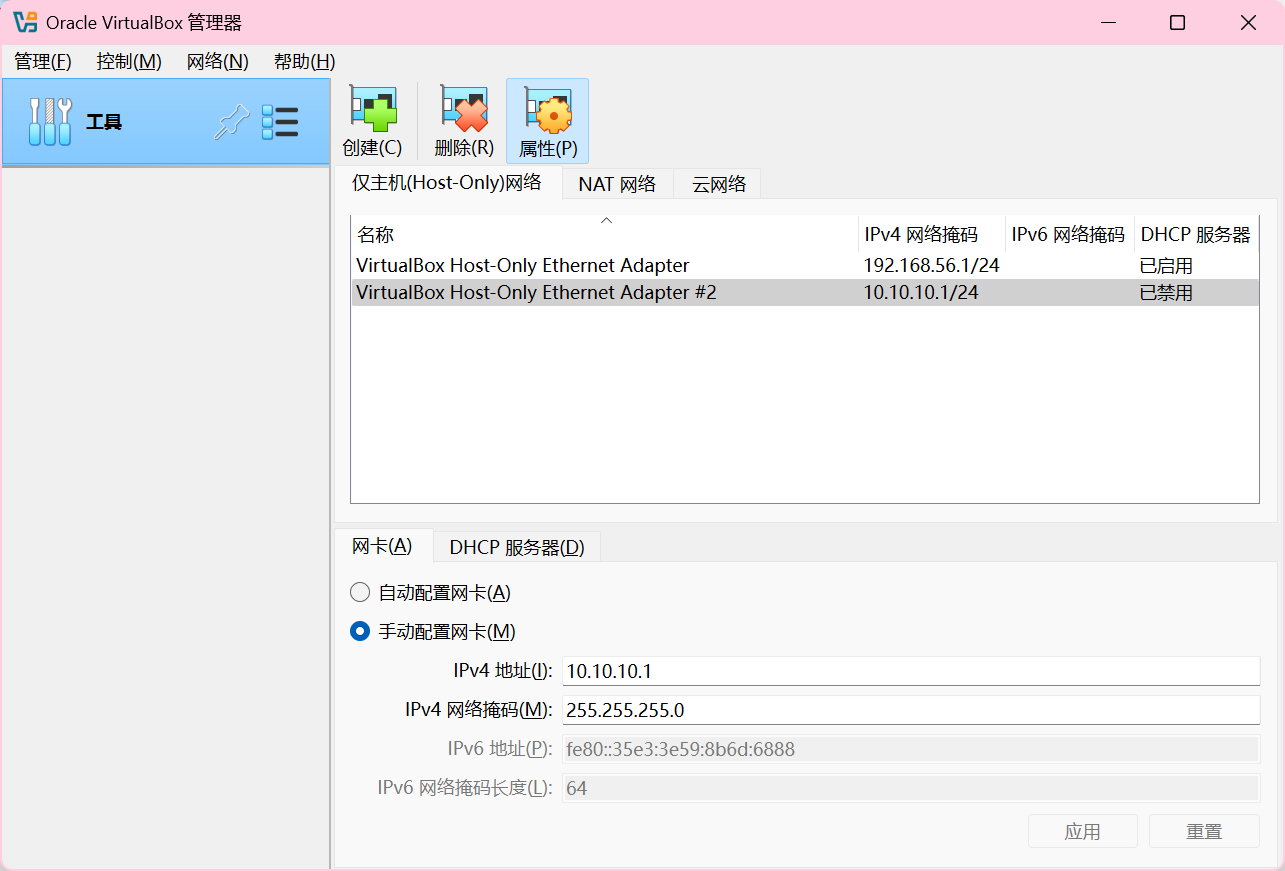
\includegraphics[width=0.8\textwidth]{img/1.1.png}
\caption{新建网络}
\end{figure}

\subsection{创建虚拟机}

在 VirtualBox 中新建一个虚拟机,设置内存和虚拟硬盘大小。

\begin{figure}[H]
    \centering
    \begin{subfigure}[b]{0.9\textwidth}
        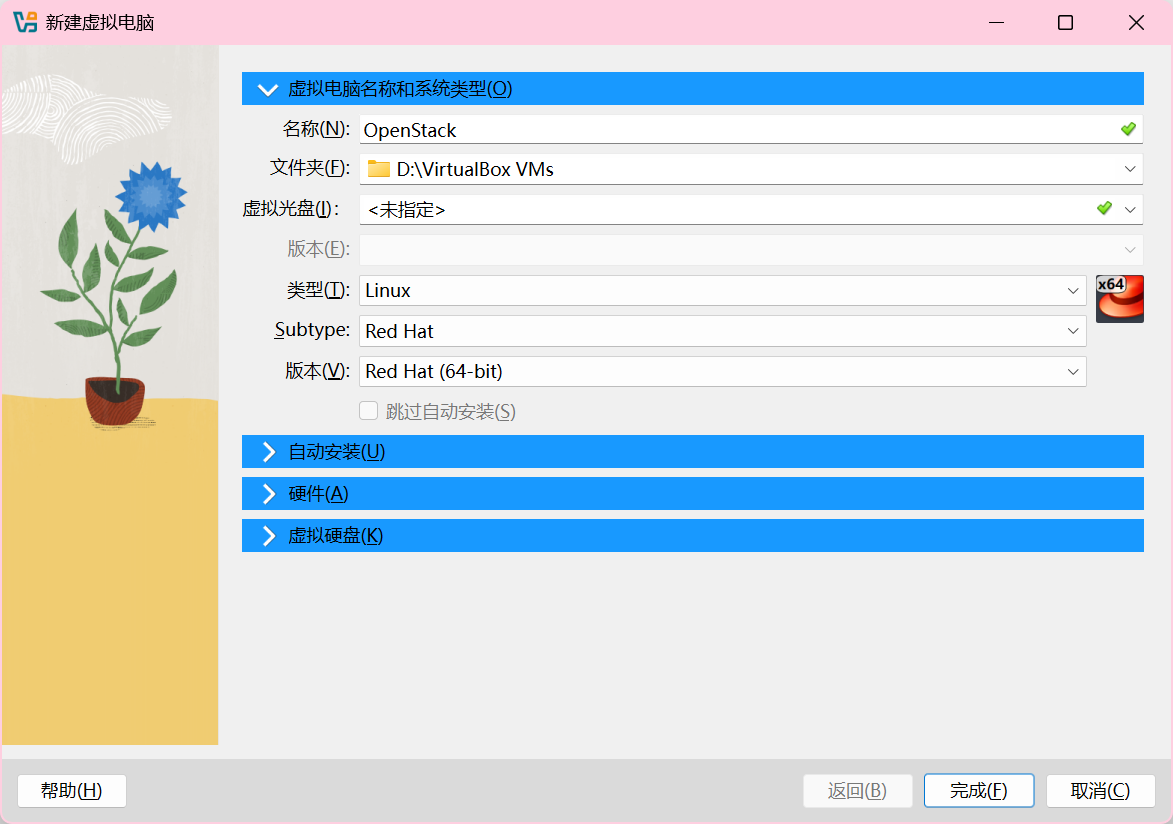
\includegraphics[width=\textwidth]{img/2.1.png}
    \end{subfigure}
    \begin{subfigure}[b]{0.45\textwidth}
        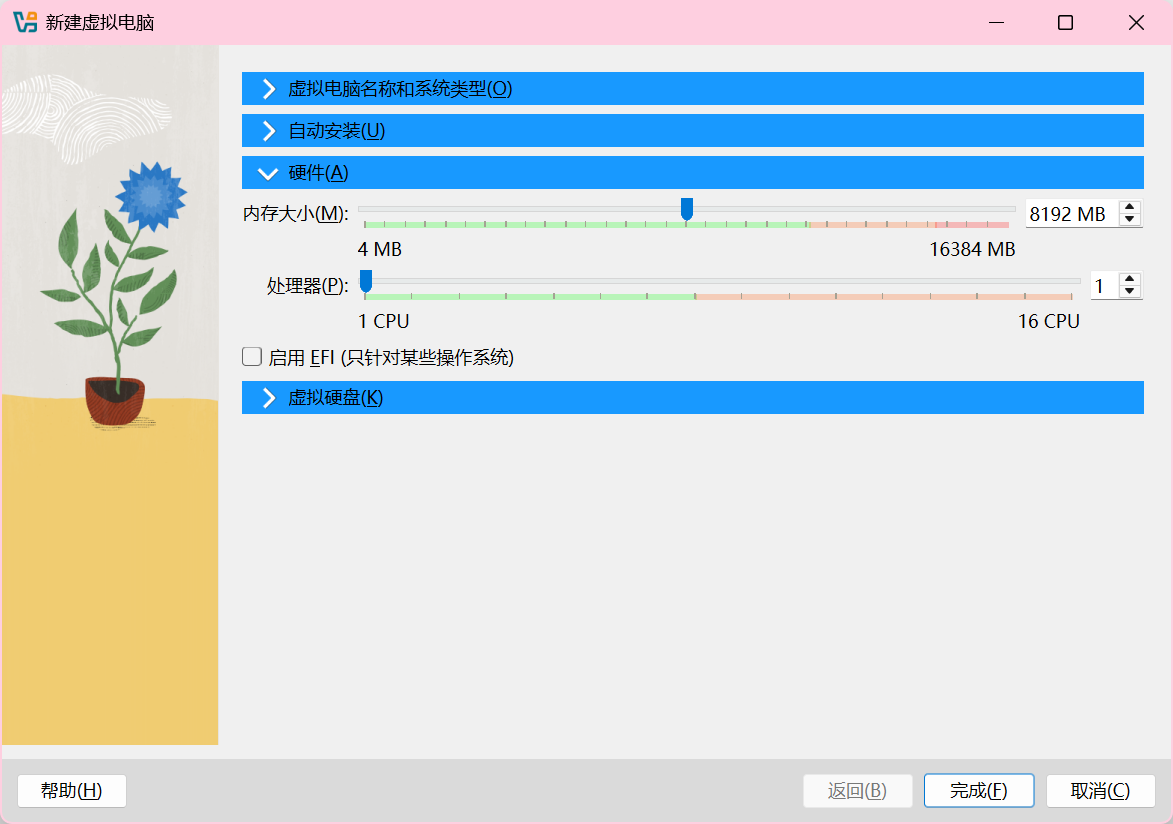
\includegraphics[width=\textwidth]{img/2.2.png}
    \end{subfigure}
    \begin{subfigure}[b]{0.45\textwidth}
        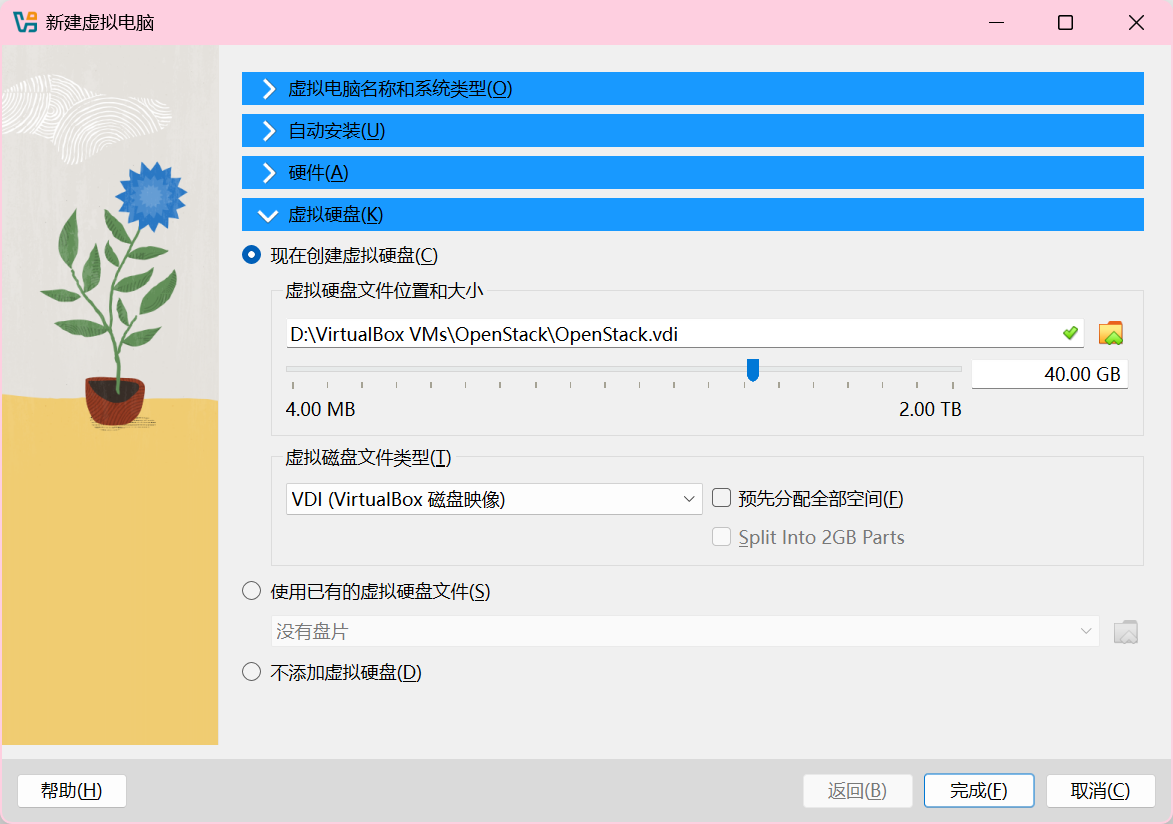
\includegraphics[width=\textwidth]{img/2.3.png}
    \end{subfigure}
    \caption{创建虚拟机}
\end{figure}

\subsection{设置网络}

进入虚拟机网络设置,设置网卡1网络连接方式为仅主机(Host-Only)网络,名称选择为刚刚新建的网络;网卡2启用网络连接,连接方式选择仅主机(Host-Only)网络,名称选择为默认网络。

\begin{figure}[H]
    \centering
    \begin{subfigure}[b]{0.45\textwidth}
        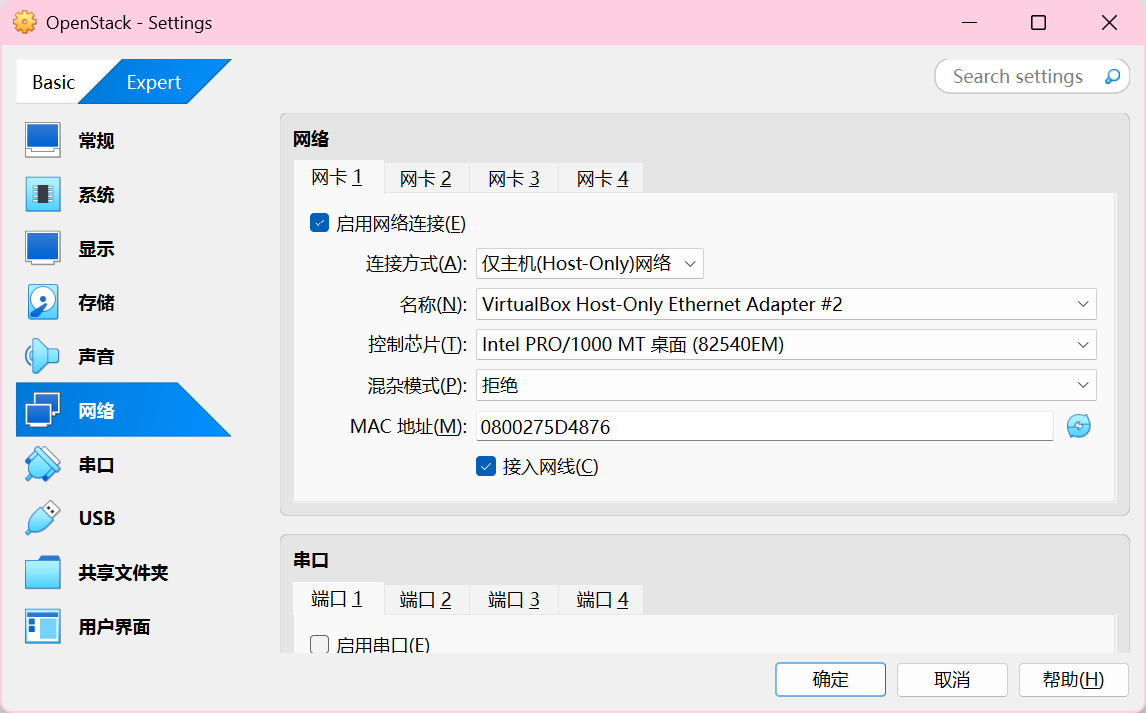
\includegraphics[width=\textwidth]{img/3.1.png}
    \end{subfigure}
    \begin{subfigure}[b]{0.45\textwidth}
        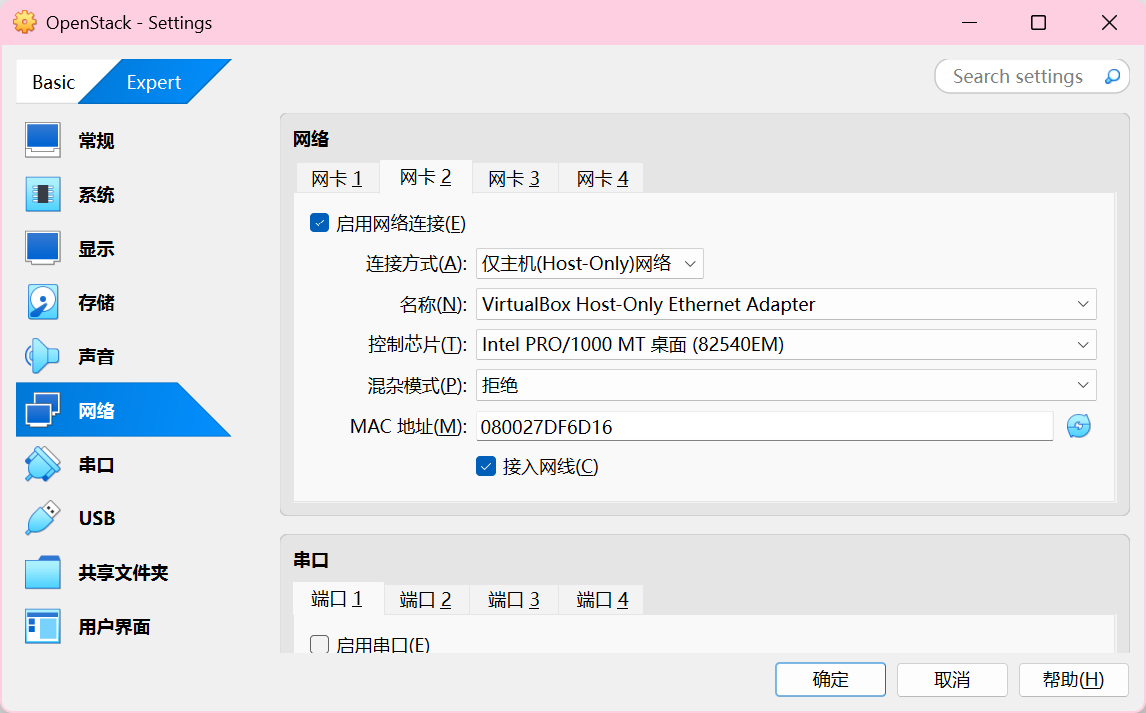
\includegraphics[width=\textwidth]{img/3.2.png}
    \end{subfigure}
    \caption{设置网络}
\end{figure}

\subsection{存储设置}

在虚拟机存储设置中,在``控制器: IDE''中选择``选择虚拟光盘文件'',选择下载的davycloud-openstack-stein.iso文件。

\begin{figure}[H]
    \centering
    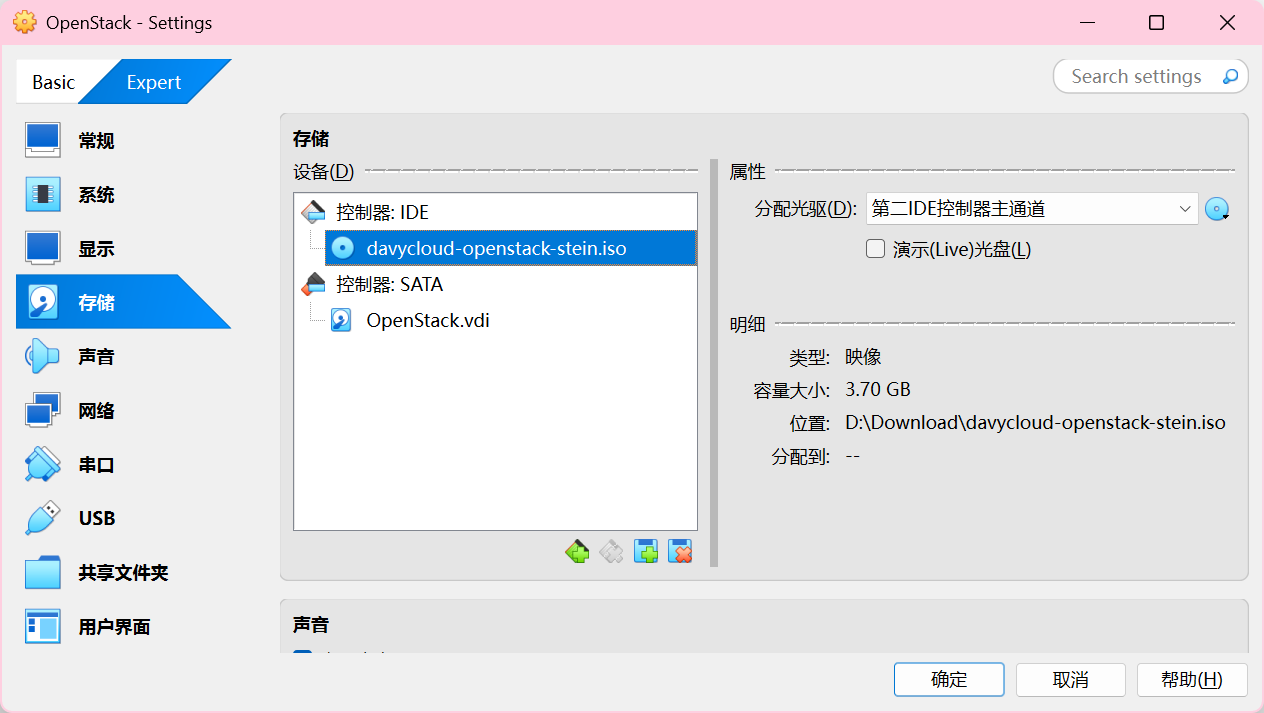
\includegraphics[width=0.8\textwidth]{img/4.1.png}
    \caption{存储设置}
\end{figure}

\subsection{其他设置}

在系统-主板设置中,将启动顺序调整为光驱、硬盘。

\begin{figure}[H]
    \centering
    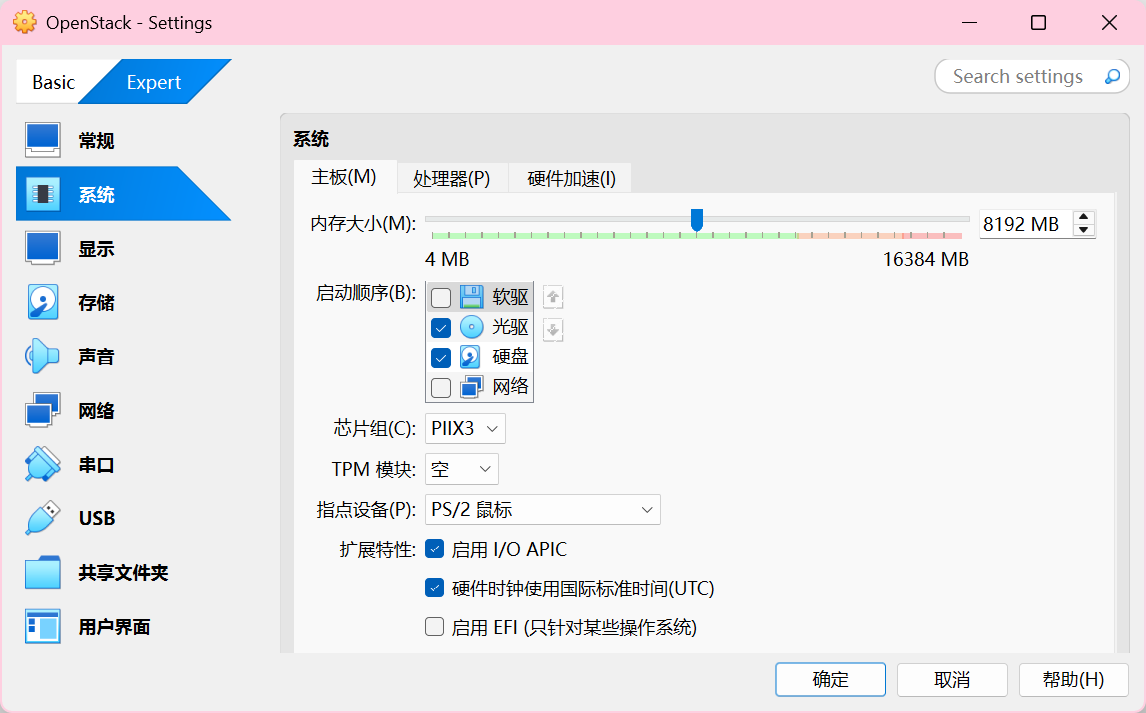
\includegraphics[width=0.75\textwidth]{img/5.1.png}
    \caption{设置启动顺序}
\end{figure}

在处理器设置中,将处理器数量适当调高。

\begin{figure}[H]
    \centering
    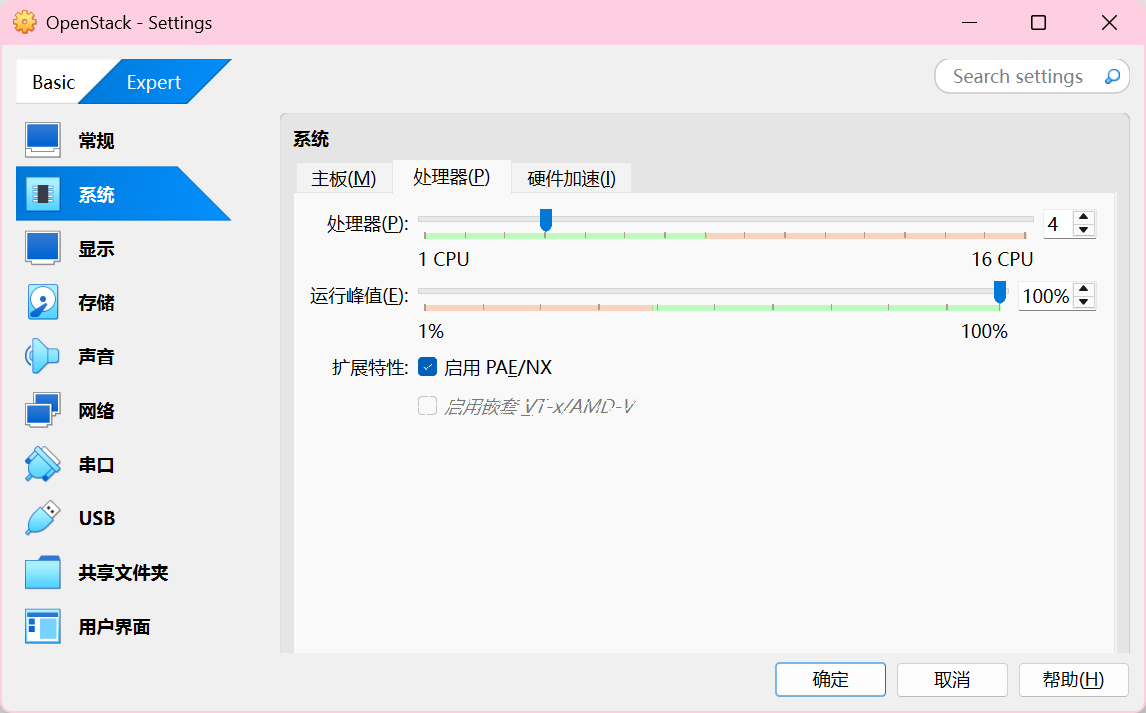
\includegraphics[width=0.75\textwidth]{img/5.2.png}
    \caption{设置处理器数量}
\end{figure}

\subsection{启动}

启动虚拟机,进入安装界面,选择第一项``Install Deploy Mode''。

\begin{figure}[H]
    \centering
    \begin{subfigure}[b]{0.45\textwidth}
        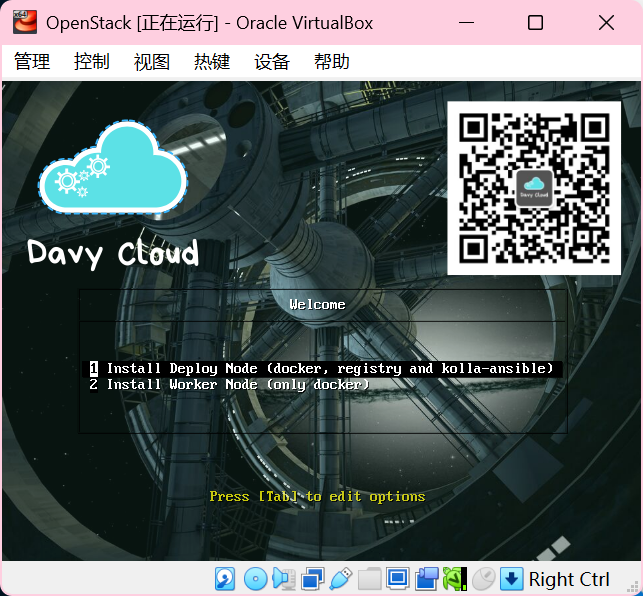
\includegraphics[width=\textwidth]{img/6.1.png}
    \end{subfigure}
    \begin{subfigure}[b]{0.45\textwidth}
        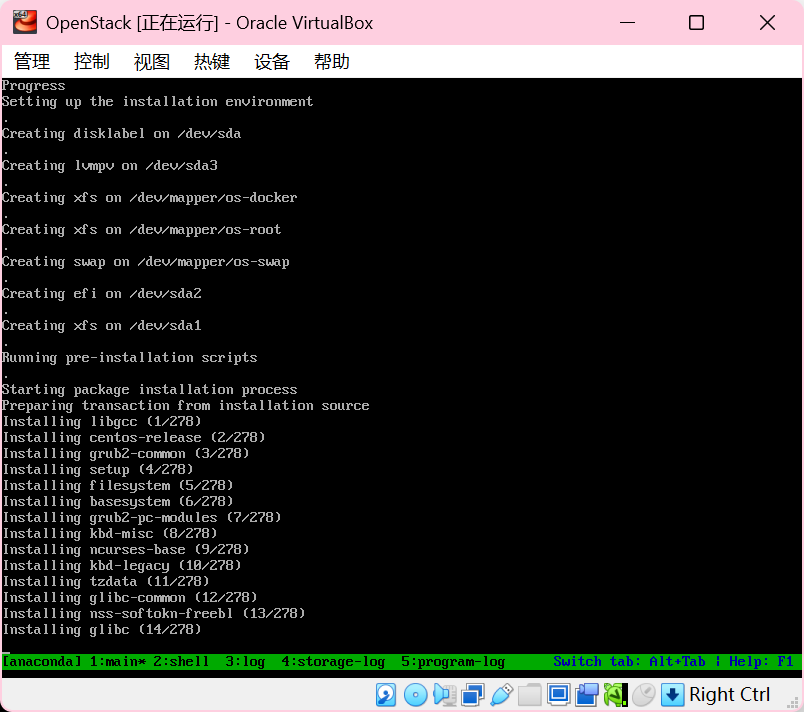
\includegraphics[width=\textwidth]{img/6.2.png}
    \end{subfigure}
    \caption{安装}
\end{figure}

等待安装完成自动重启后,输入用户名(kolla)和密码(kollapass,输入时不会显示)登录。

\begin{figure}[H]
    \centering
    \begin{subfigure}[b]{0.45\textwidth}
        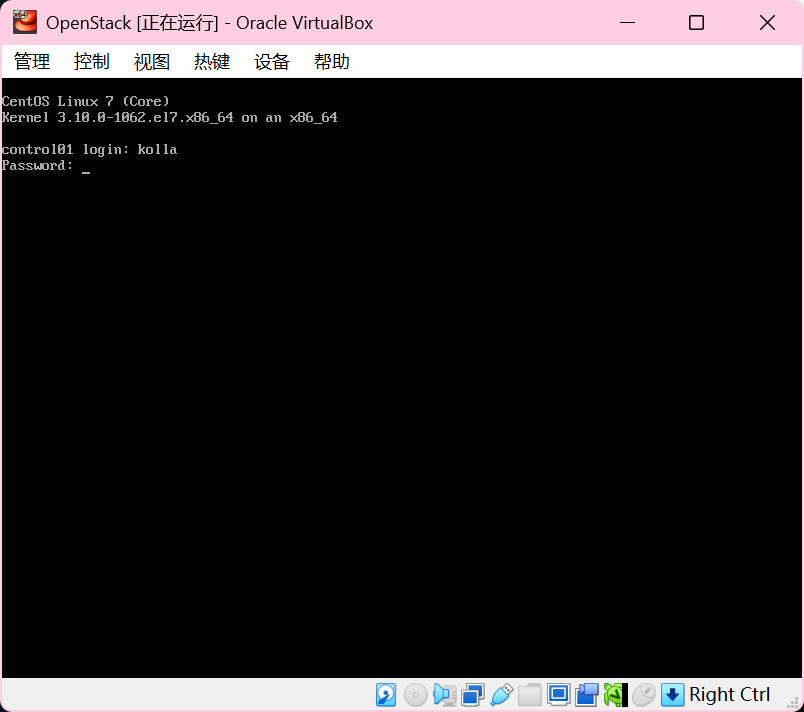
\includegraphics[width=\textwidth]{img/6.3.png}
    \end{subfigure}
    \begin{subfigure}[b]{0.45\textwidth}
        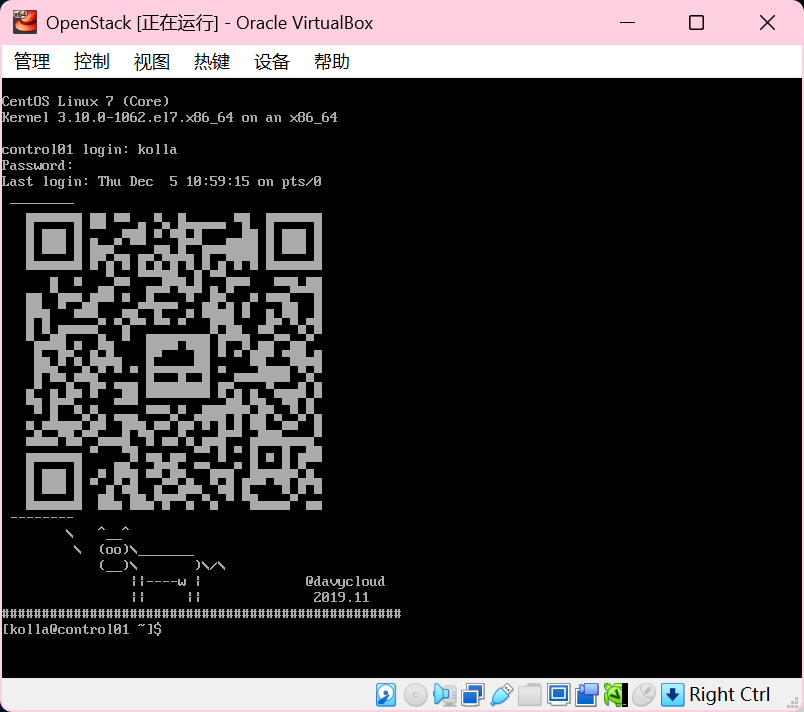
\includegraphics[width=\textwidth]{img/6.4.png}
    \end{subfigure}
    \caption{登录}
\end{figure}

使用 \texttt{sudo -s} 切换到 root 用户。输入 \texttt{kolla-ansible} 查看\texttt{kolla-ansible}工具是否安装成功。

\begin{lstlisting}[language=bash]
    sudo -s
    kolla-ansible
\end{lstlisting}

\begin{figure}[H]
    \centering
    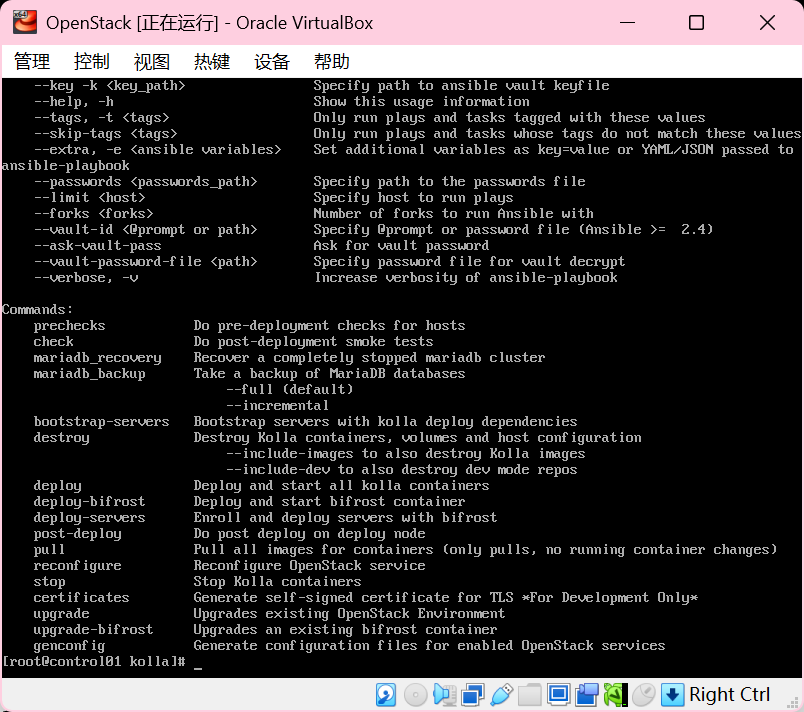
\includegraphics[width=0.47\textwidth]{img/6.5.png}
    \caption{查看kolla-ansible}
\end{figure}

\subsection{安装OpenStack}

使用 \texttt{kolla-ansible} 进行预检查。

\begin{lstlisting}[language=bash]
    kolla-ansible prechecks
\end{lstlisting}

\begin{figure}[H]
    \centering
    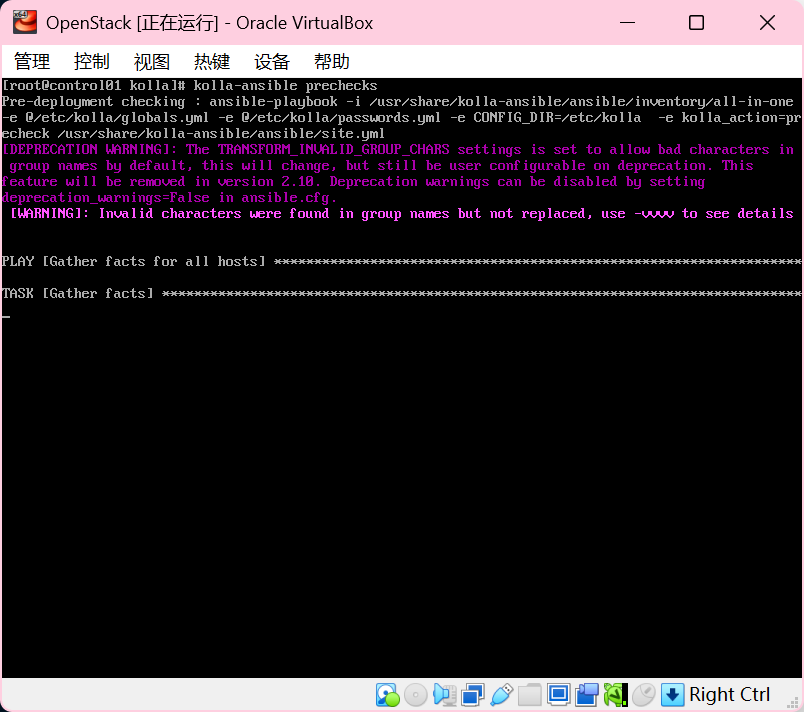
\includegraphics[width=0.47\textwidth]{img/7.1.png}
    \caption{预检查}
\end{figure}

输入命令 \texttt{kolla-ansible deploy} 开始安装OpenStack。

\begin{lstlisting}[language=bash]
    kolla-ansible deploy
\end{lstlisting}

\begin{figure}[H]
    \centering
    \begin{subfigure}[b]{0.47\textwidth}
        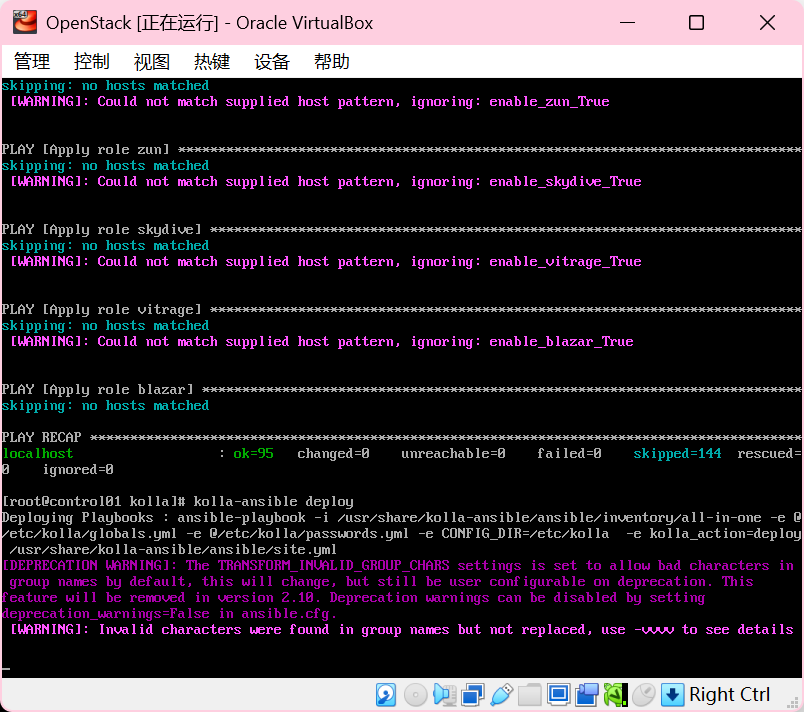
\includegraphics[width=\textwidth]{img/7.2.png}
    \end{subfigure}
    \begin{subfigure}[b]{0.47\textwidth}
        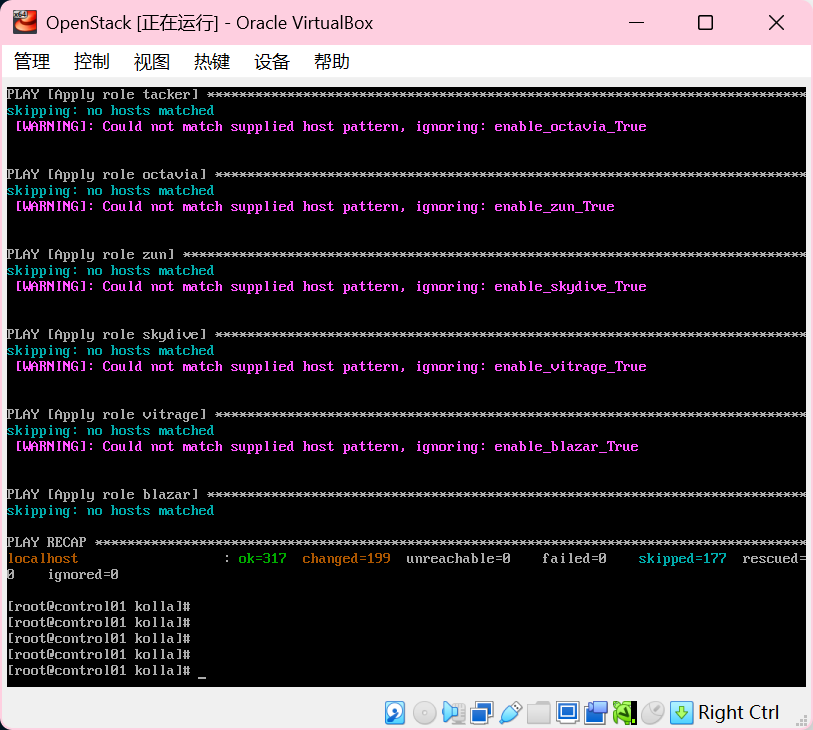
\includegraphics[width=\textwidth]{img/7.3.png}
    \end{subfigure}
    \caption{安装OpenStack}
\end{figure}

输入 \texttt{kolla-ansible post-deploy} 生成IC文件。

\begin{lstlisting}[language=bash]
    kolla-ansible post-deploy
\end{lstlisting}

\begin{figure}[H]
    \centering
    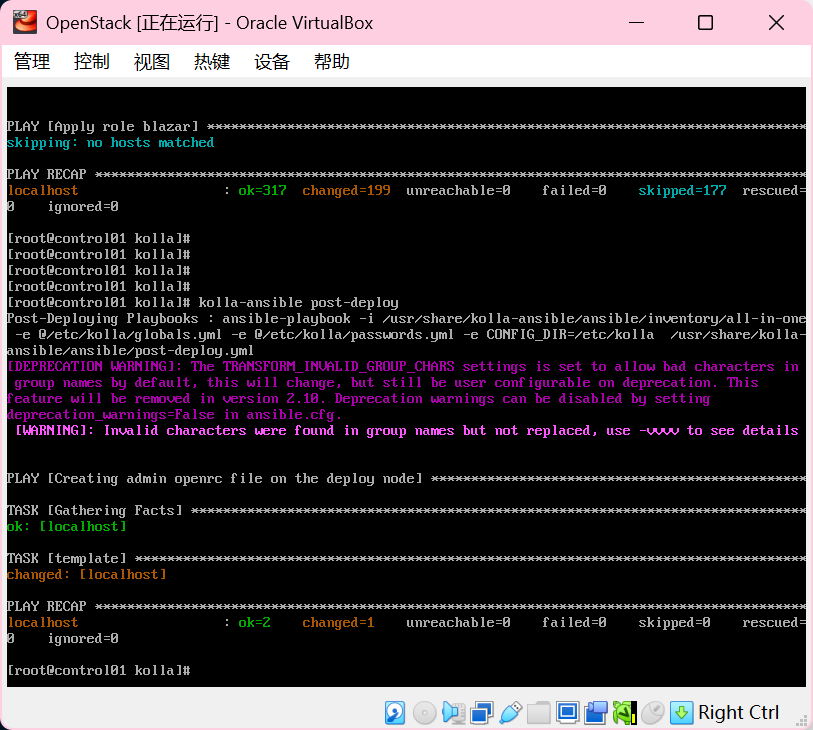
\includegraphics[width=0.47\textwidth]{img/7.4.png}
    \caption{生成IC文件}
\end{figure}

获取 admin 权限,然后运行 openstack。

\begin{lstlisting}[language=bash]
    source /etc/kolla/admin-openrc.sh
    openstack
\end{lstlisting}

\begin{figure}[H]
    \centering
    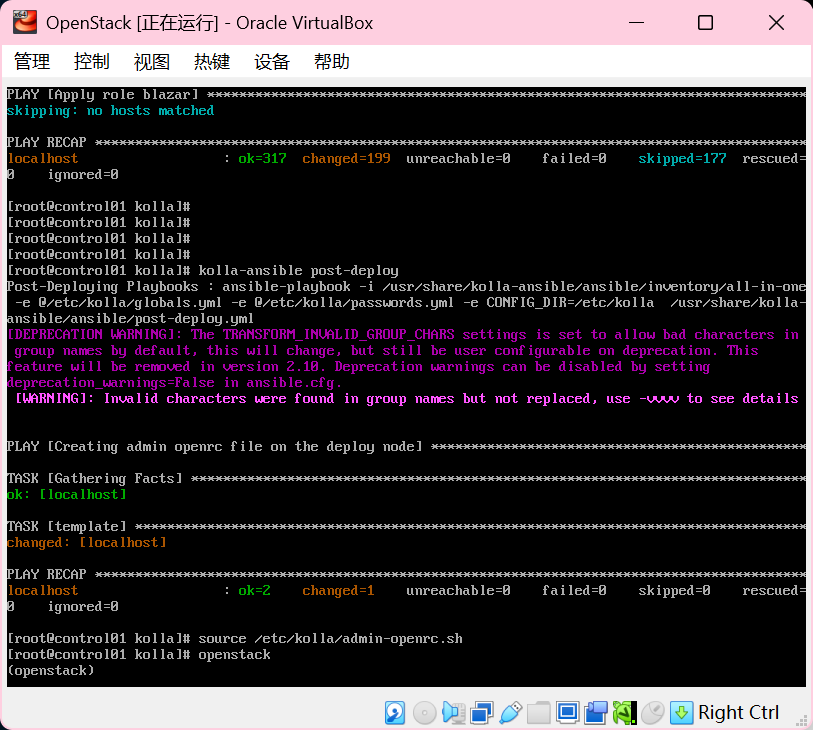
\includegraphics[width=0.45\textwidth]{img/7.5.png}
    \caption{运行openstack}
\end{figure}

输入 \texttt{service list} 查看服务列表。

\begin{lstlisting}[language=bash]
    (openstack) service list
\end{lstlisting}

\begin{figure}[H]
    \centering
    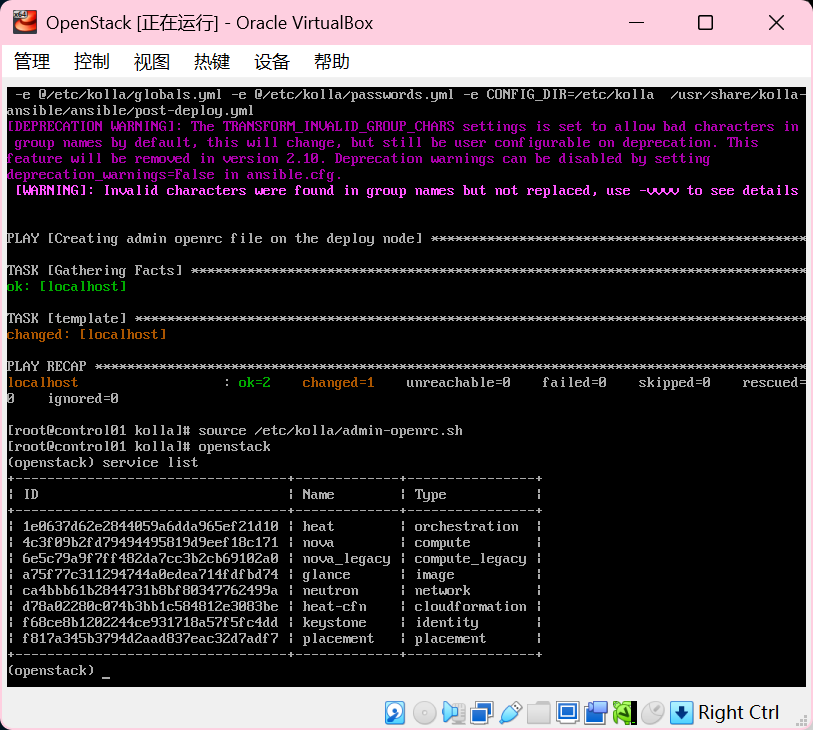
\includegraphics[width=0.45\textwidth]{img/7.6.png}
    \caption{查看服务列表}
\end{figure}

按 \texttt{Ctrl + D} 退出 openstack 后,查看密码。

\begin{lstlisting}[language=bash]
    cat /etc/kolla/admin-openrc.sh
\end{lstlisting}

\begin{figure}[H]
    \centering
    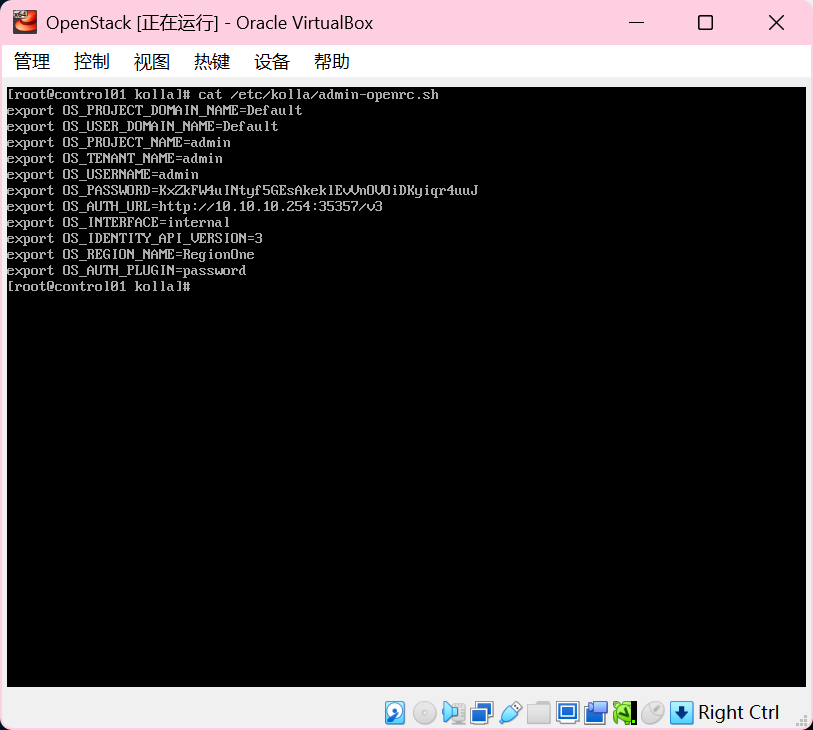
\includegraphics[width=0.8\textwidth]{img/7.7.png}
    \caption{查看密码}
\end{figure}

可以看到密码为\texttt{KxZkFW4uINtyf5GEsAkeklEvVnOVOiDKyiqr4uuJ}。

在浏览器中输入 \texttt{10.10.10.2} 进入 OpenStack 界面,输入用户名\texttt{admin}和刚刚查看到的密码登录。

\begin{figure}[H]
    \centering
    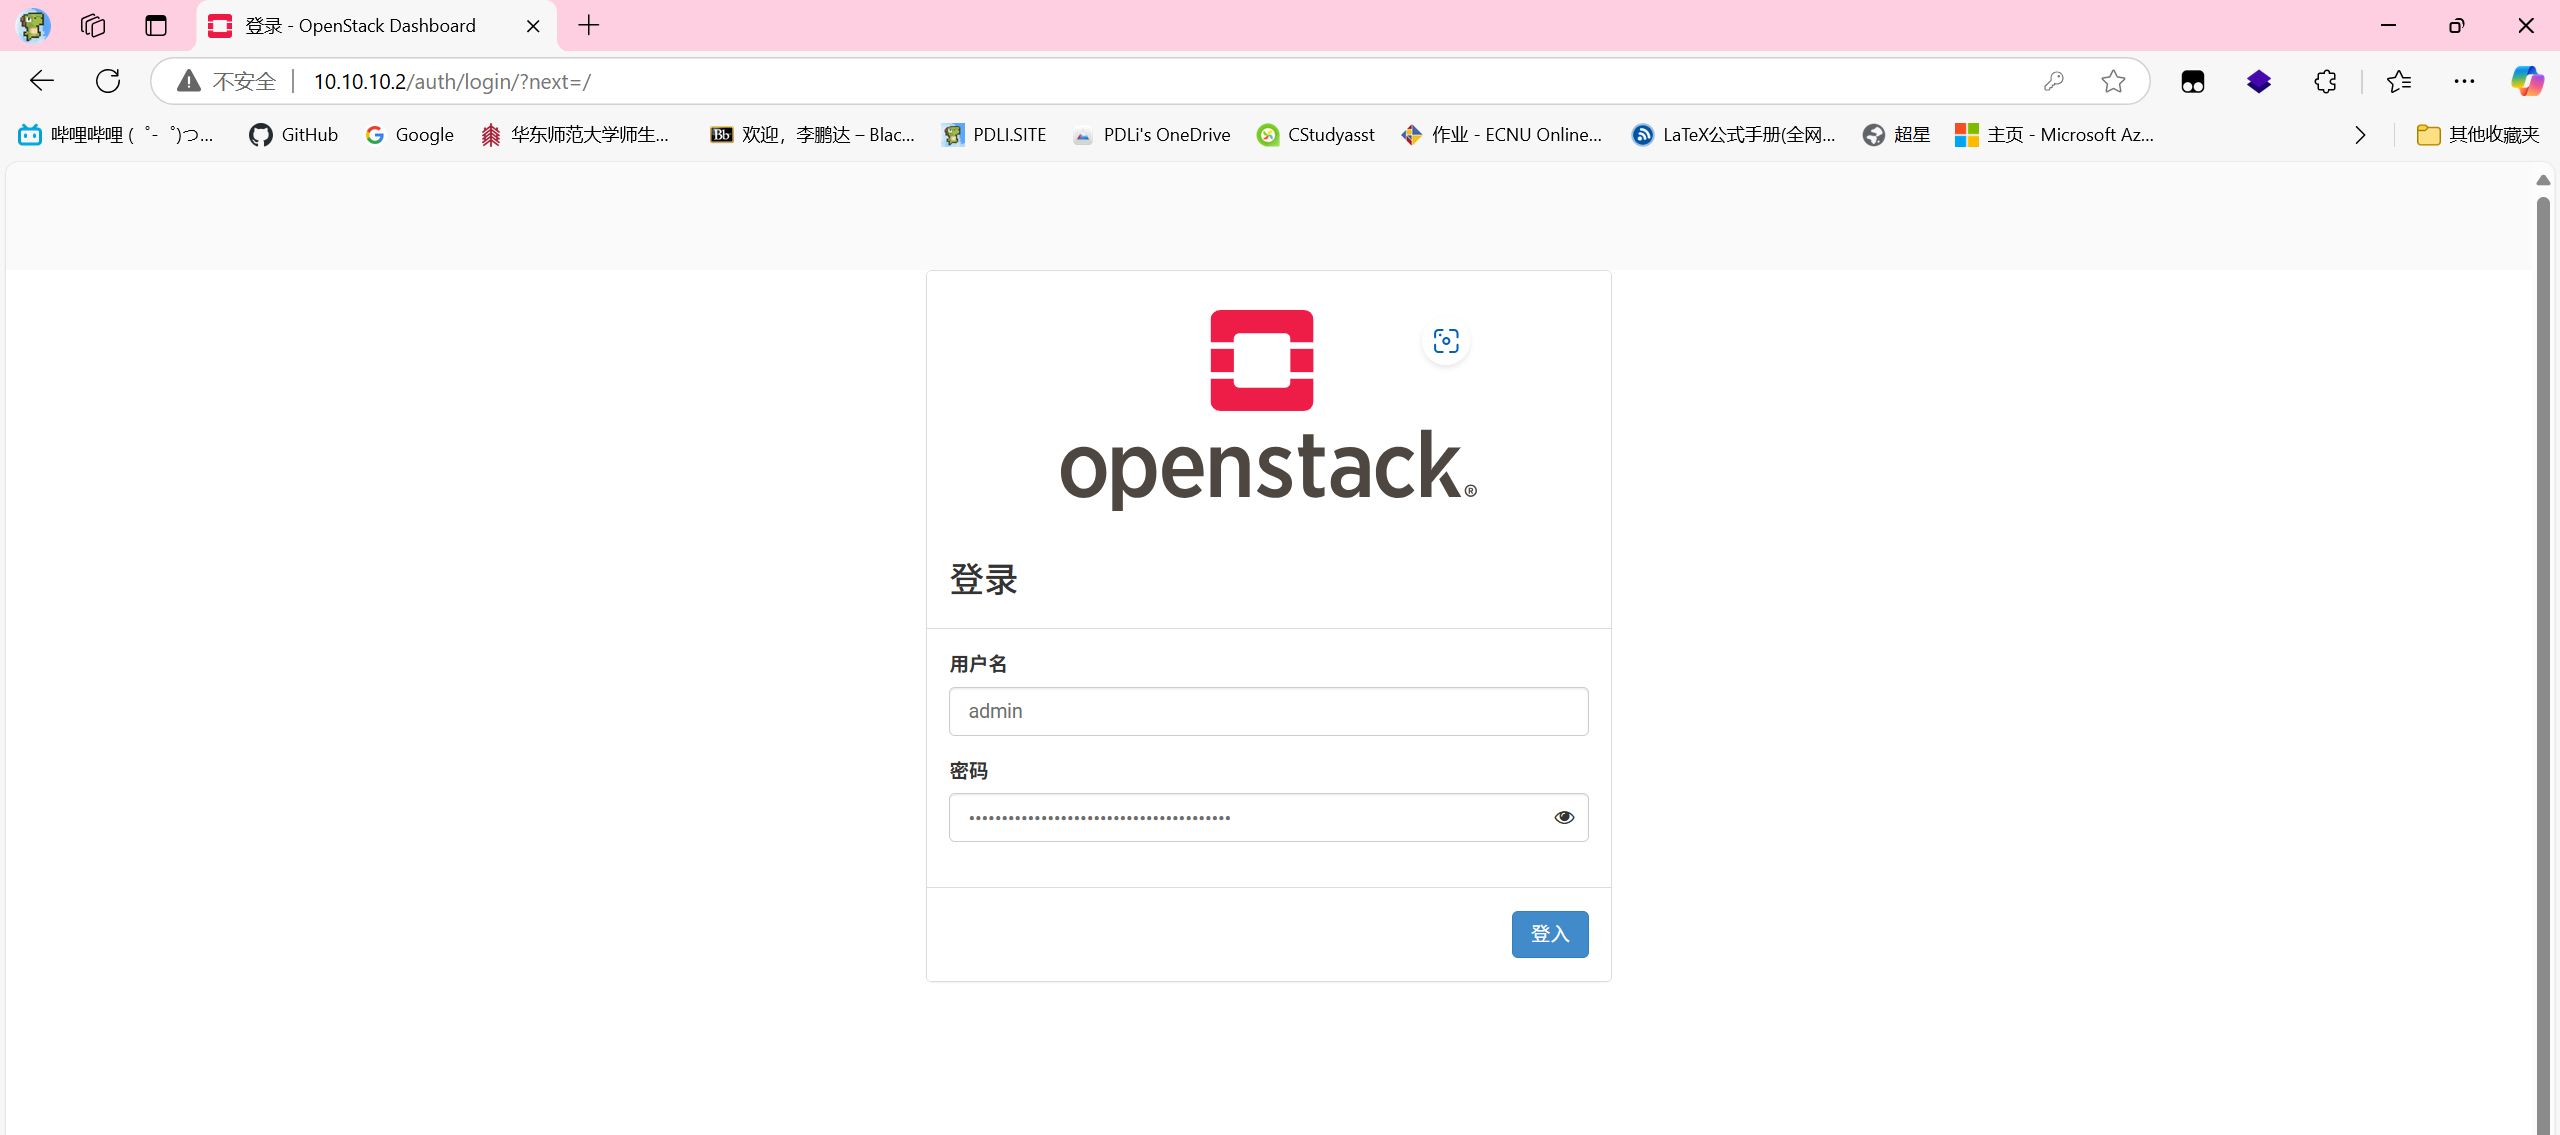
\includegraphics[width=0.8\textwidth]{img/7.8.png}
    \caption{登录OpenStack}
\end{figure}

登陆后,可以看到 OpenStack 的控制台。

\begin{figure}[H]
    \centering
    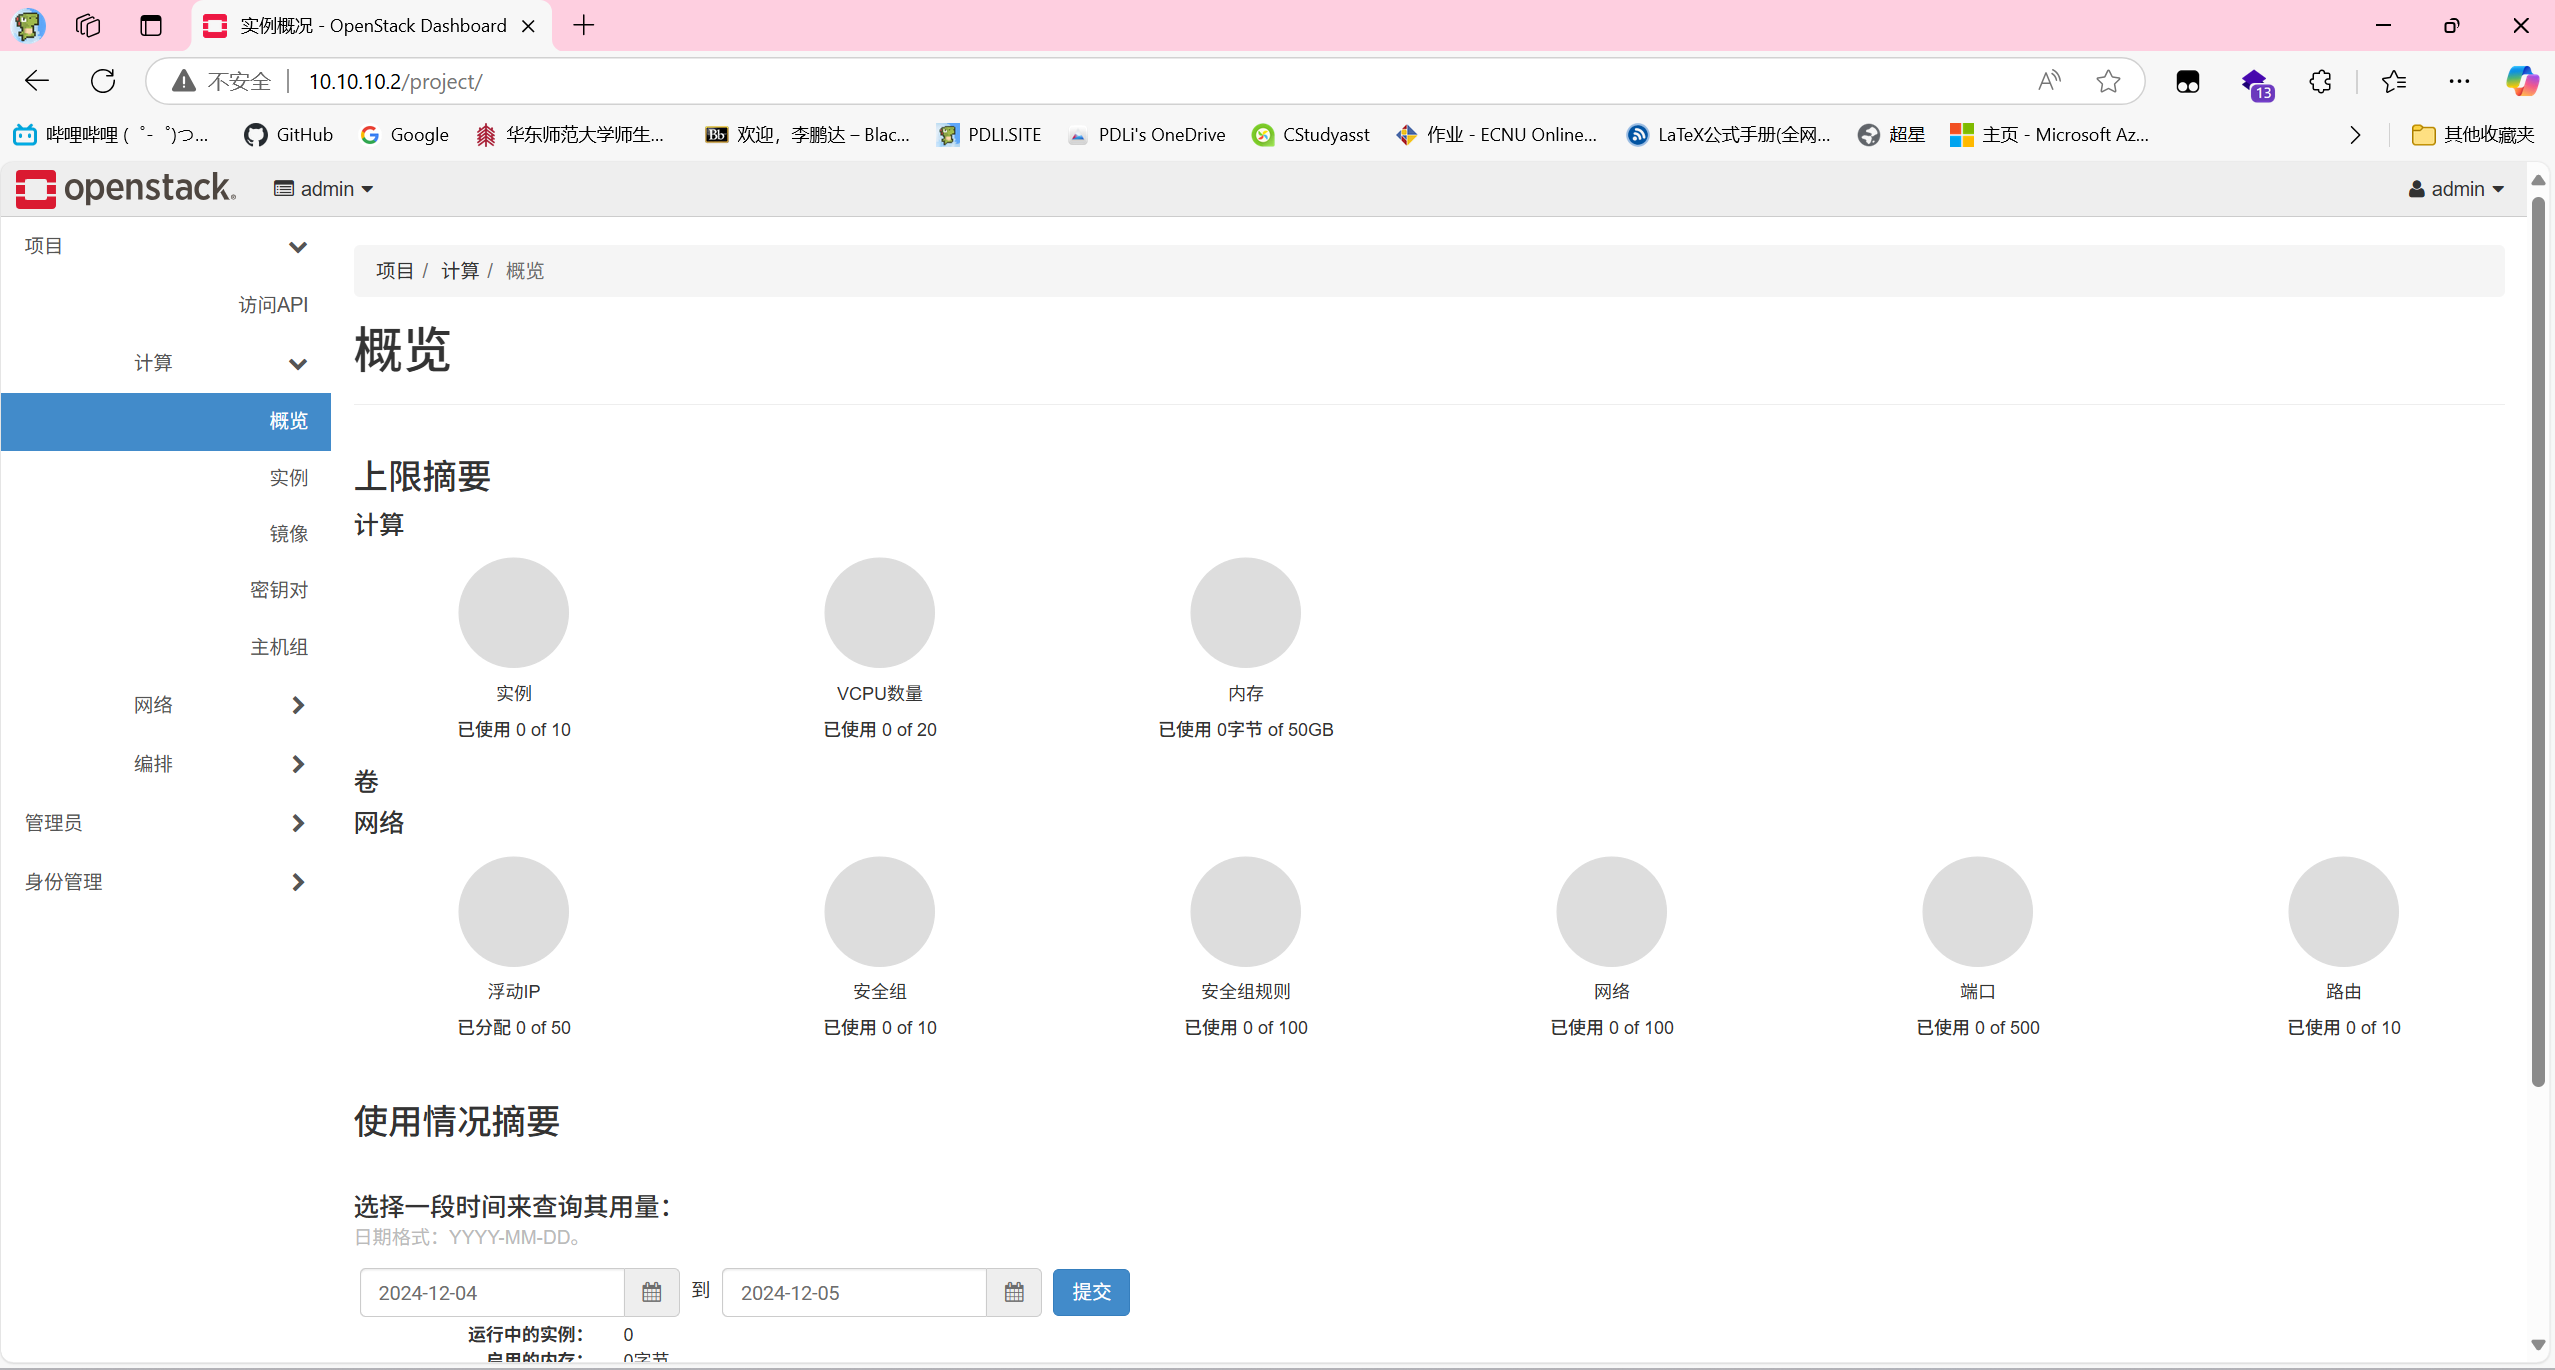
\includegraphics[width=0.8\textwidth]{img/7.9.png}
    \caption{OpenStack控制台}
\end{figure}

查看一些系统信息。

\begin{figure}[H]
    \centering
    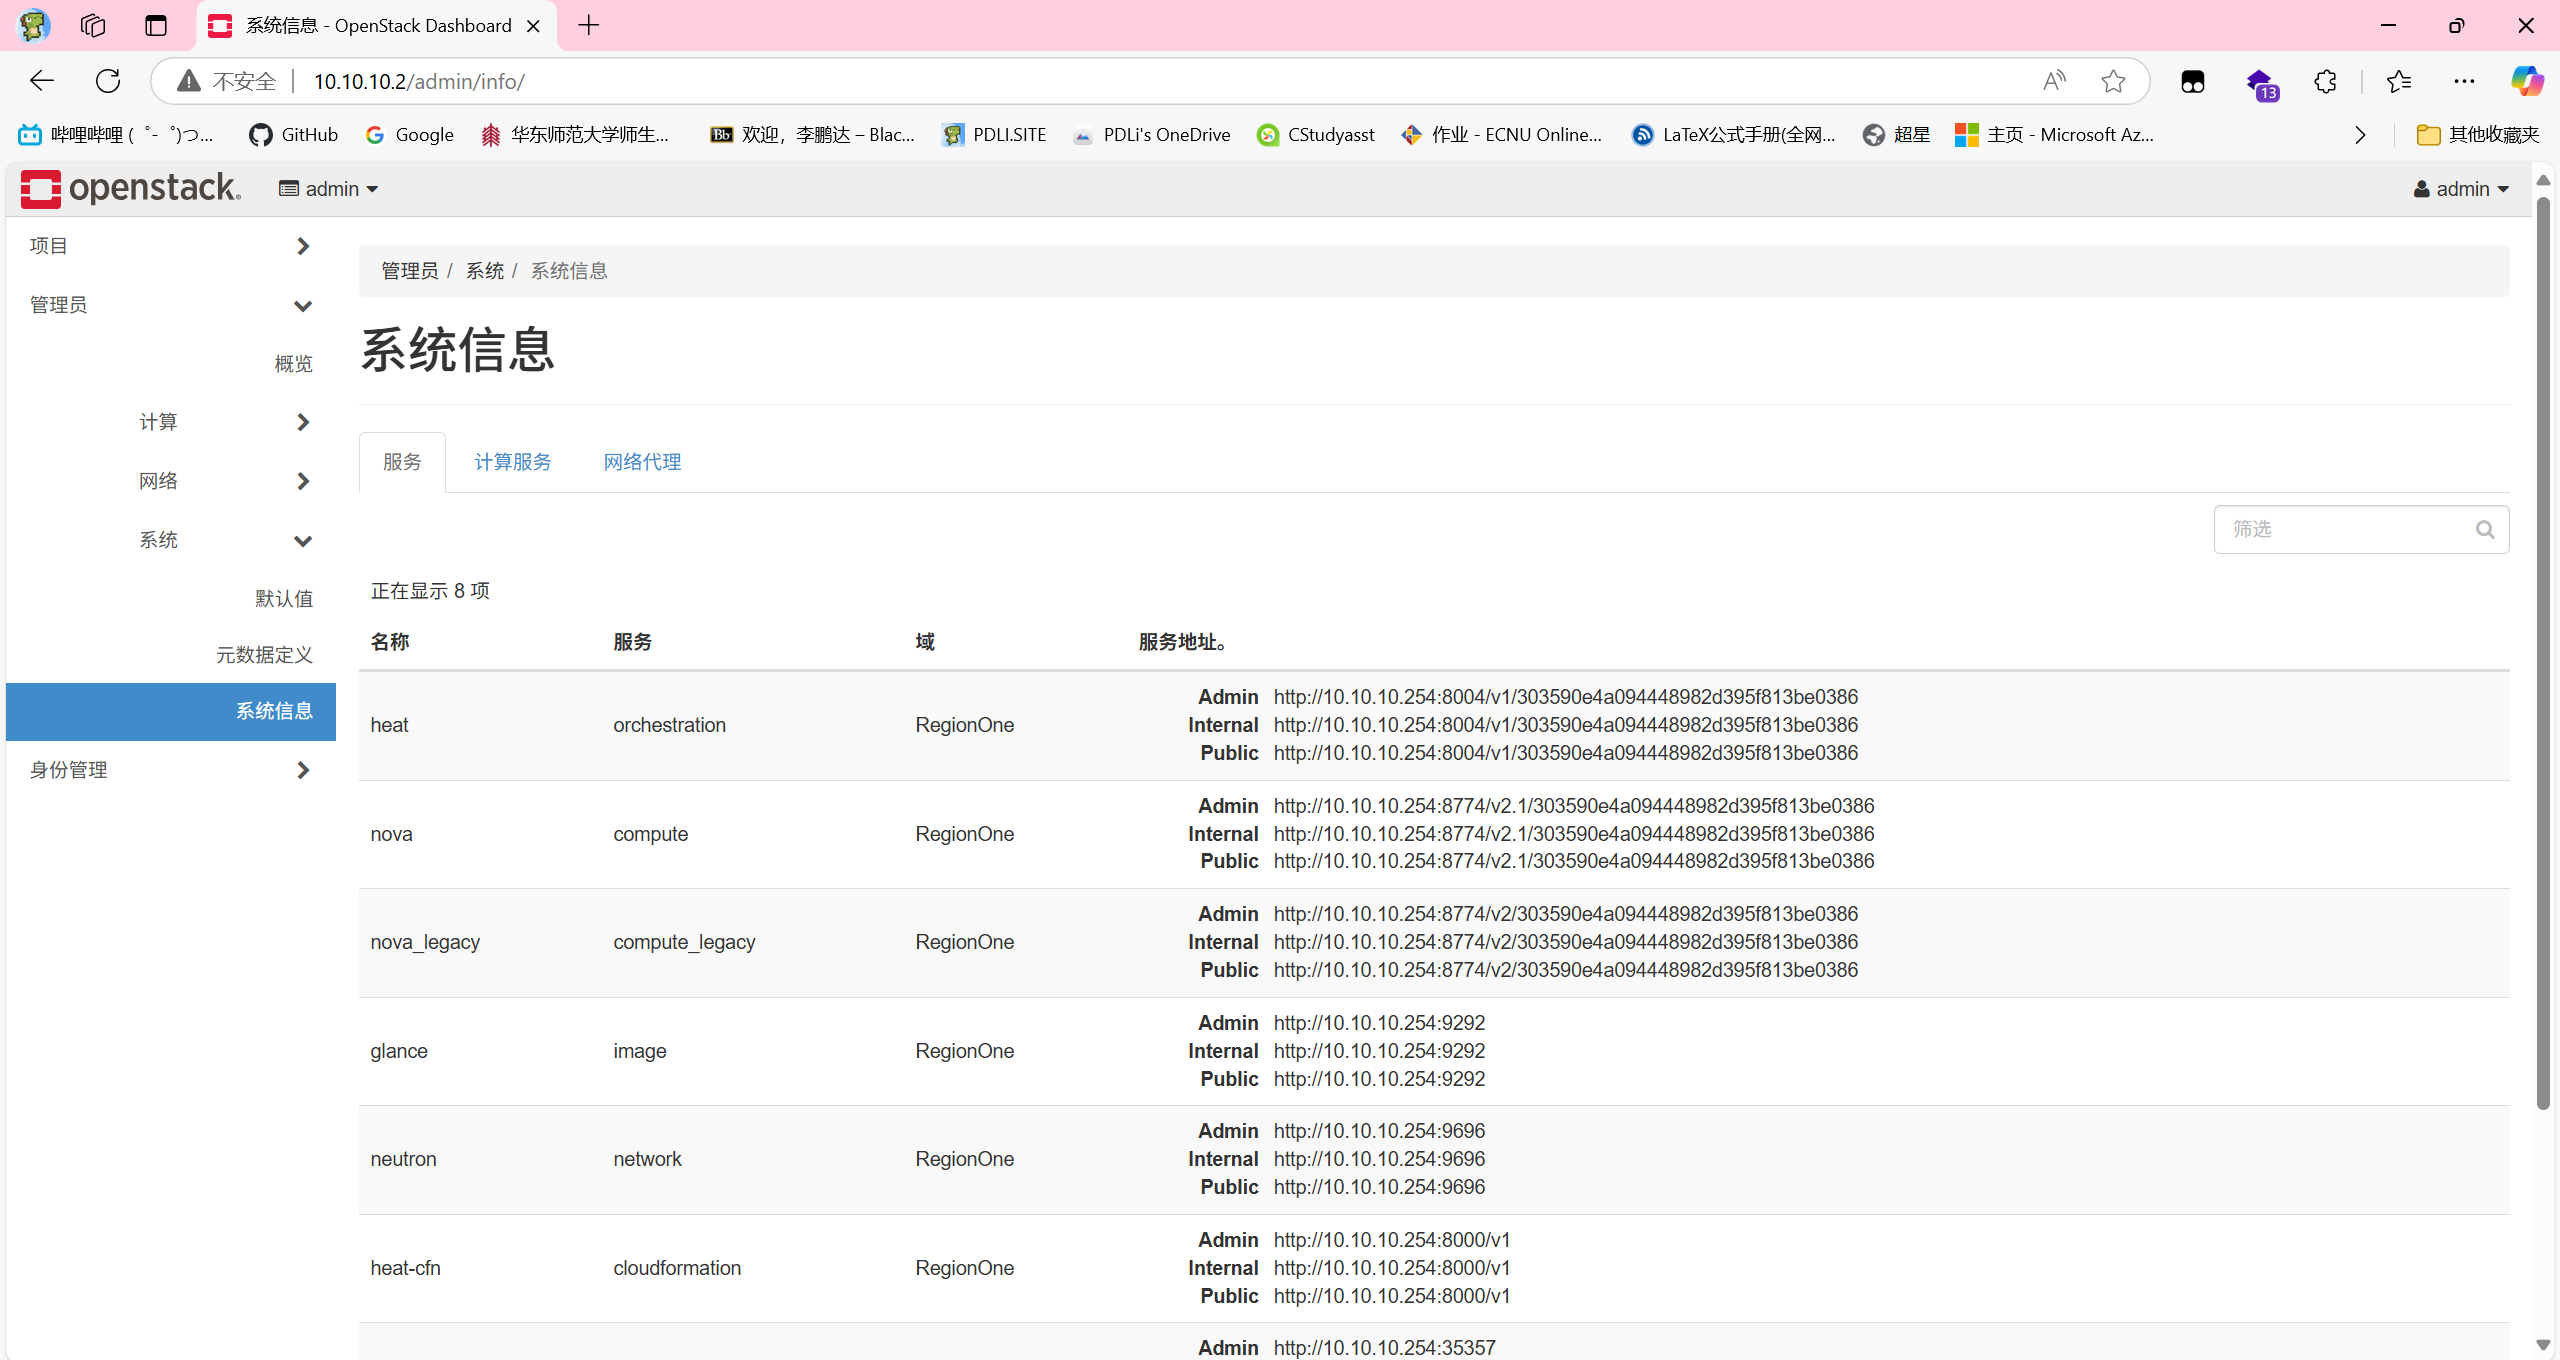
\includegraphics[width=0.8\textwidth]{img/7.10.png}
    \caption{系统信息}
\end{figure}

\subsubsection{创建镜像}

在 OpenStack 中创建一个镜像,使用下载的镜像源。

\begin{figure}[H]
    \centering
    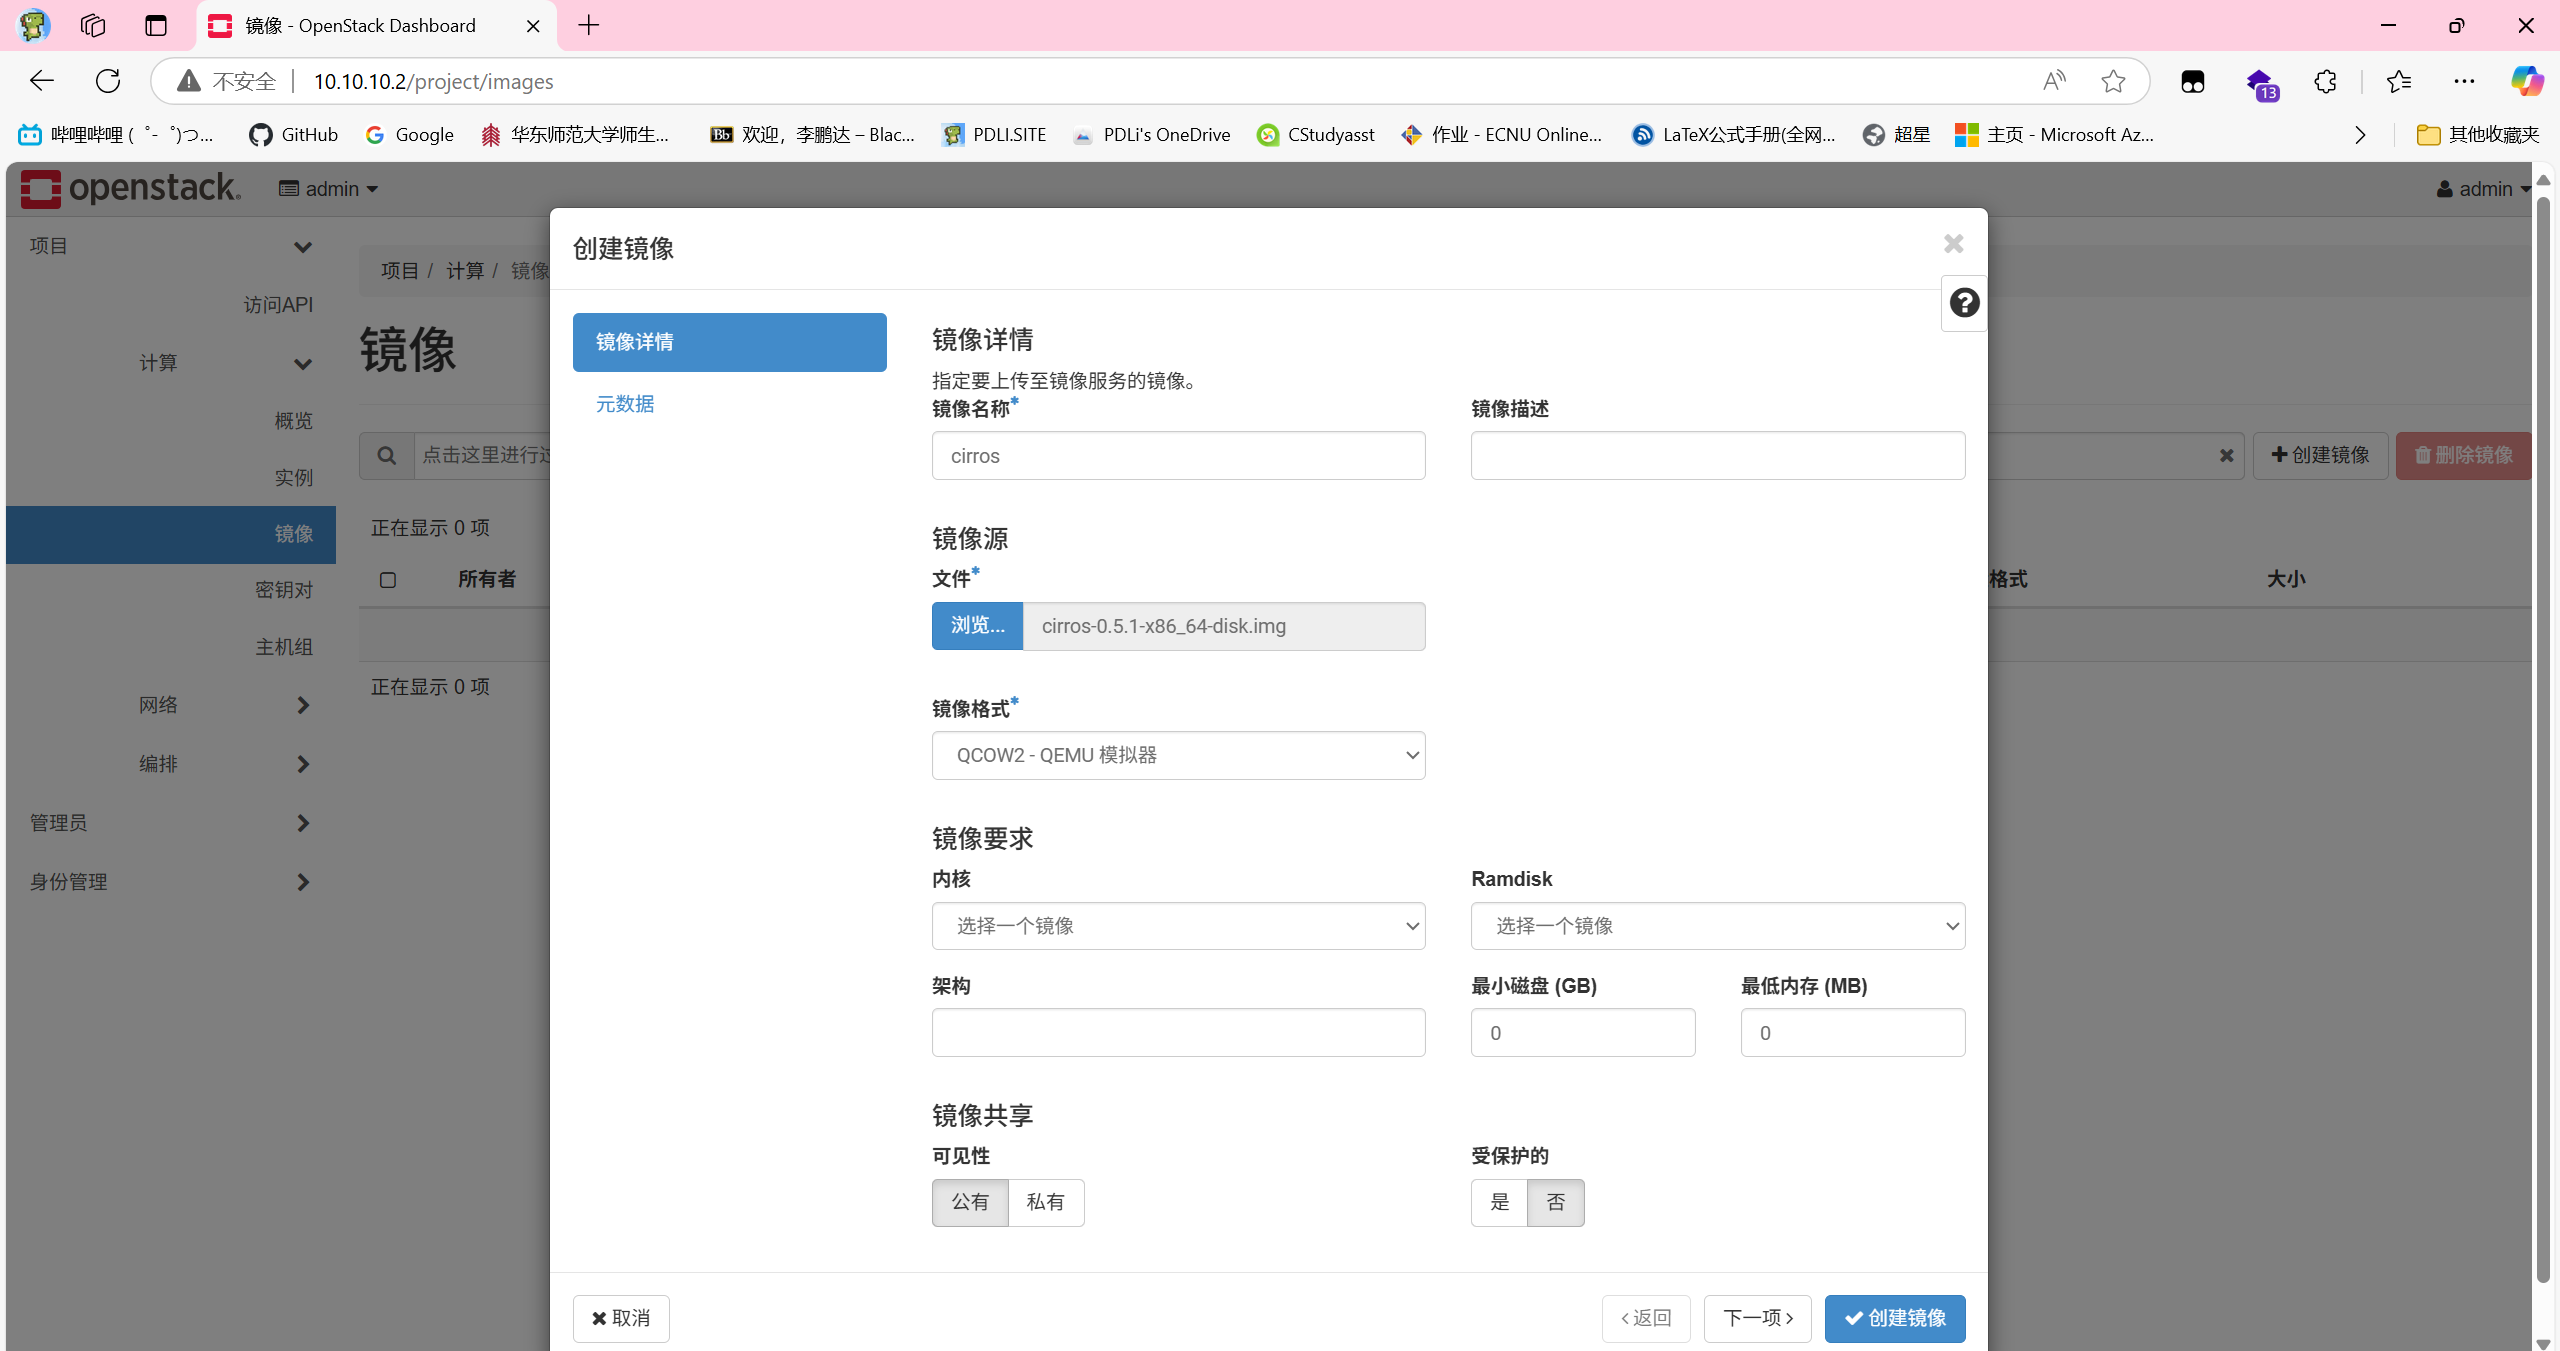
\includegraphics[width=0.8\textwidth]{img/8.1.png}
    \caption{创建镜像}
\end{figure}

\begin{figure}[H]
    \centering
    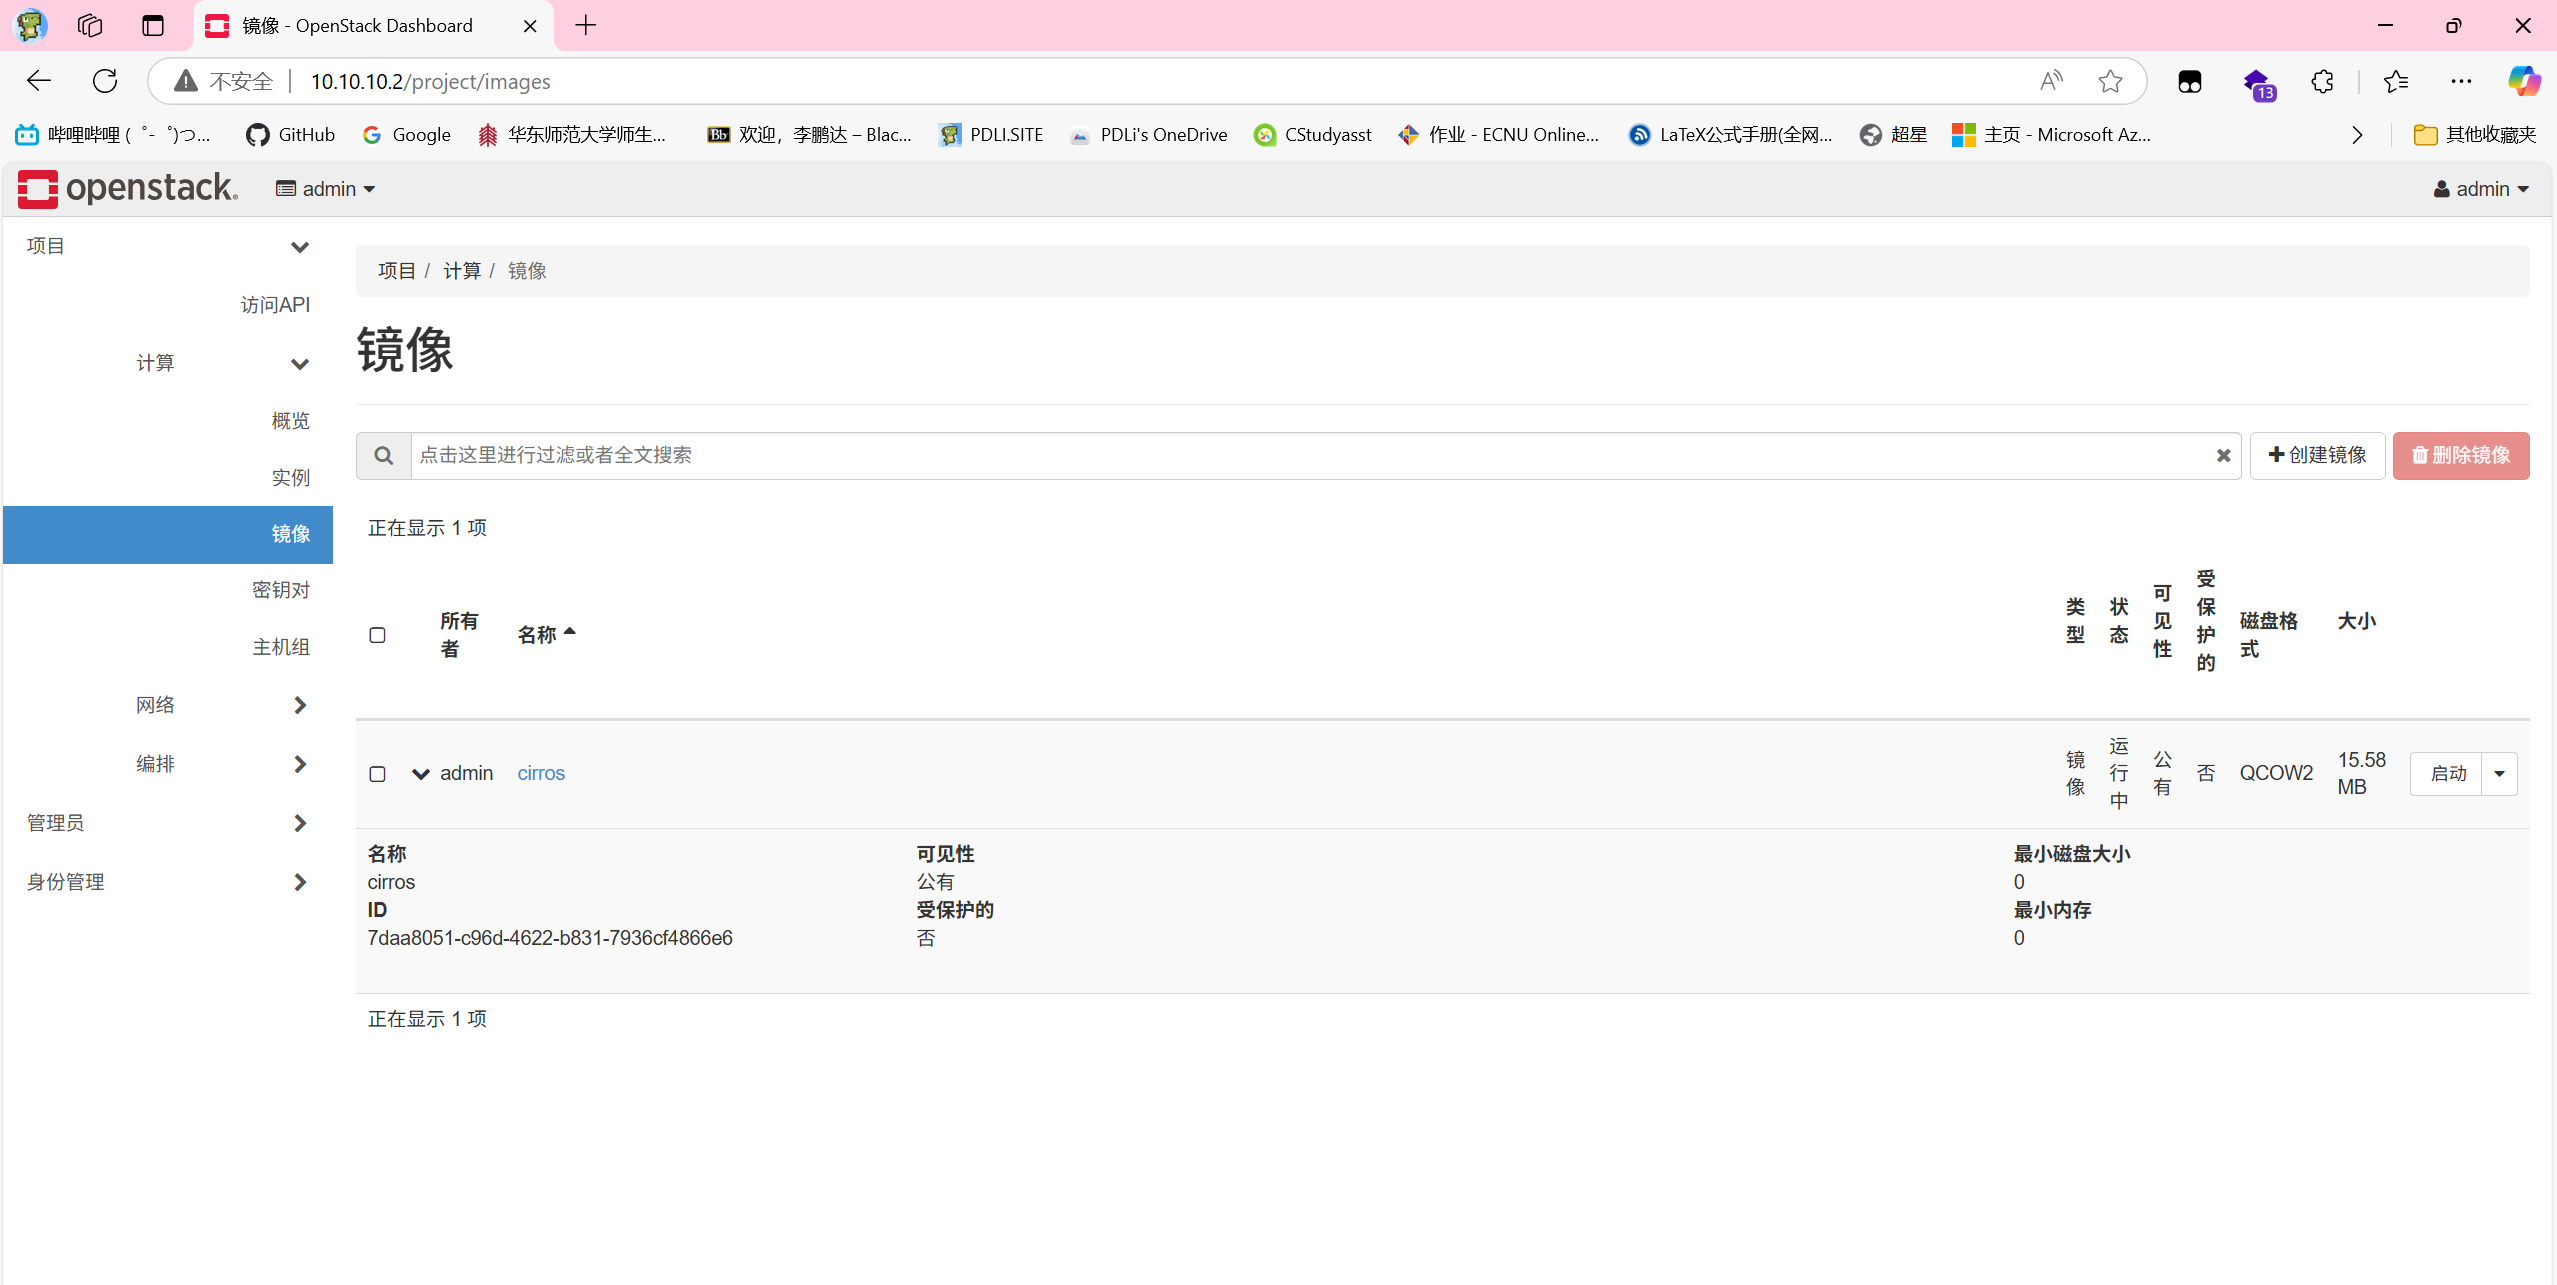
\includegraphics[width=0.8\textwidth]{img/8.2.png}
    \caption{镜像创建结果}
\end{figure}

\subsubsection{创建实例类型}

在 OpenStack 中创建一个实例类型。

\begin{figure}[H]
    \centering
    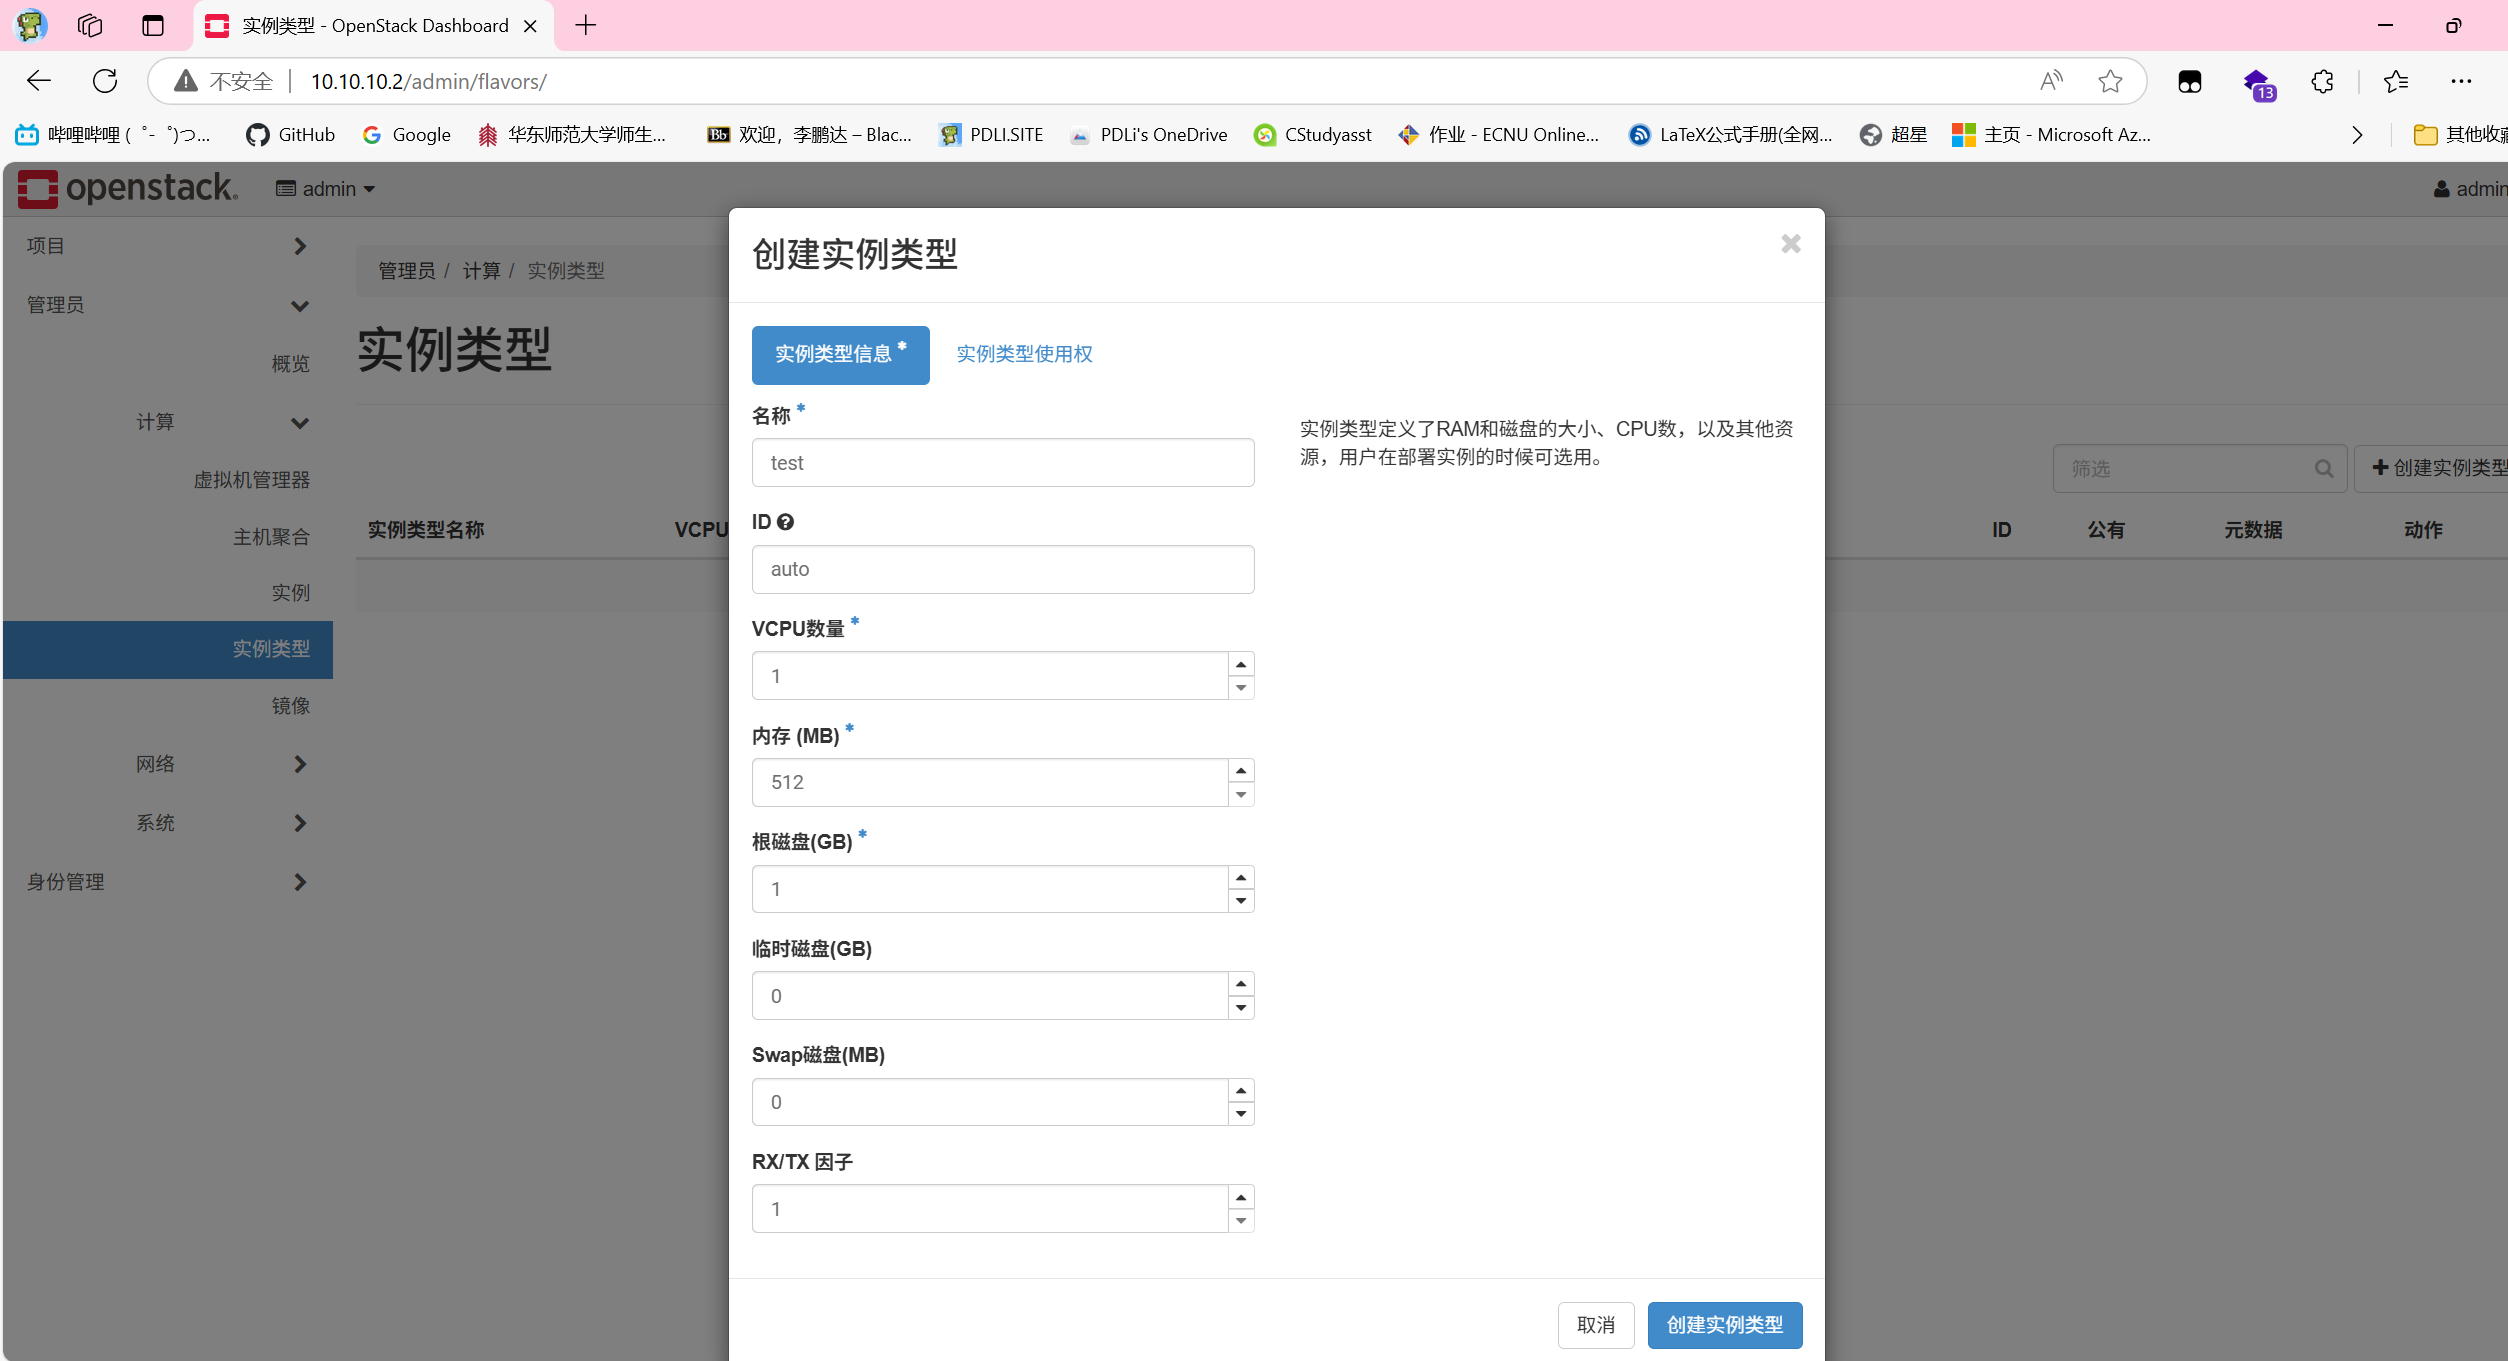
\includegraphics[width=0.8\textwidth]{img/9.1.png}
    \caption{创建实例类型}
\end{figure}

\begin{figure}[H]
    \centering
    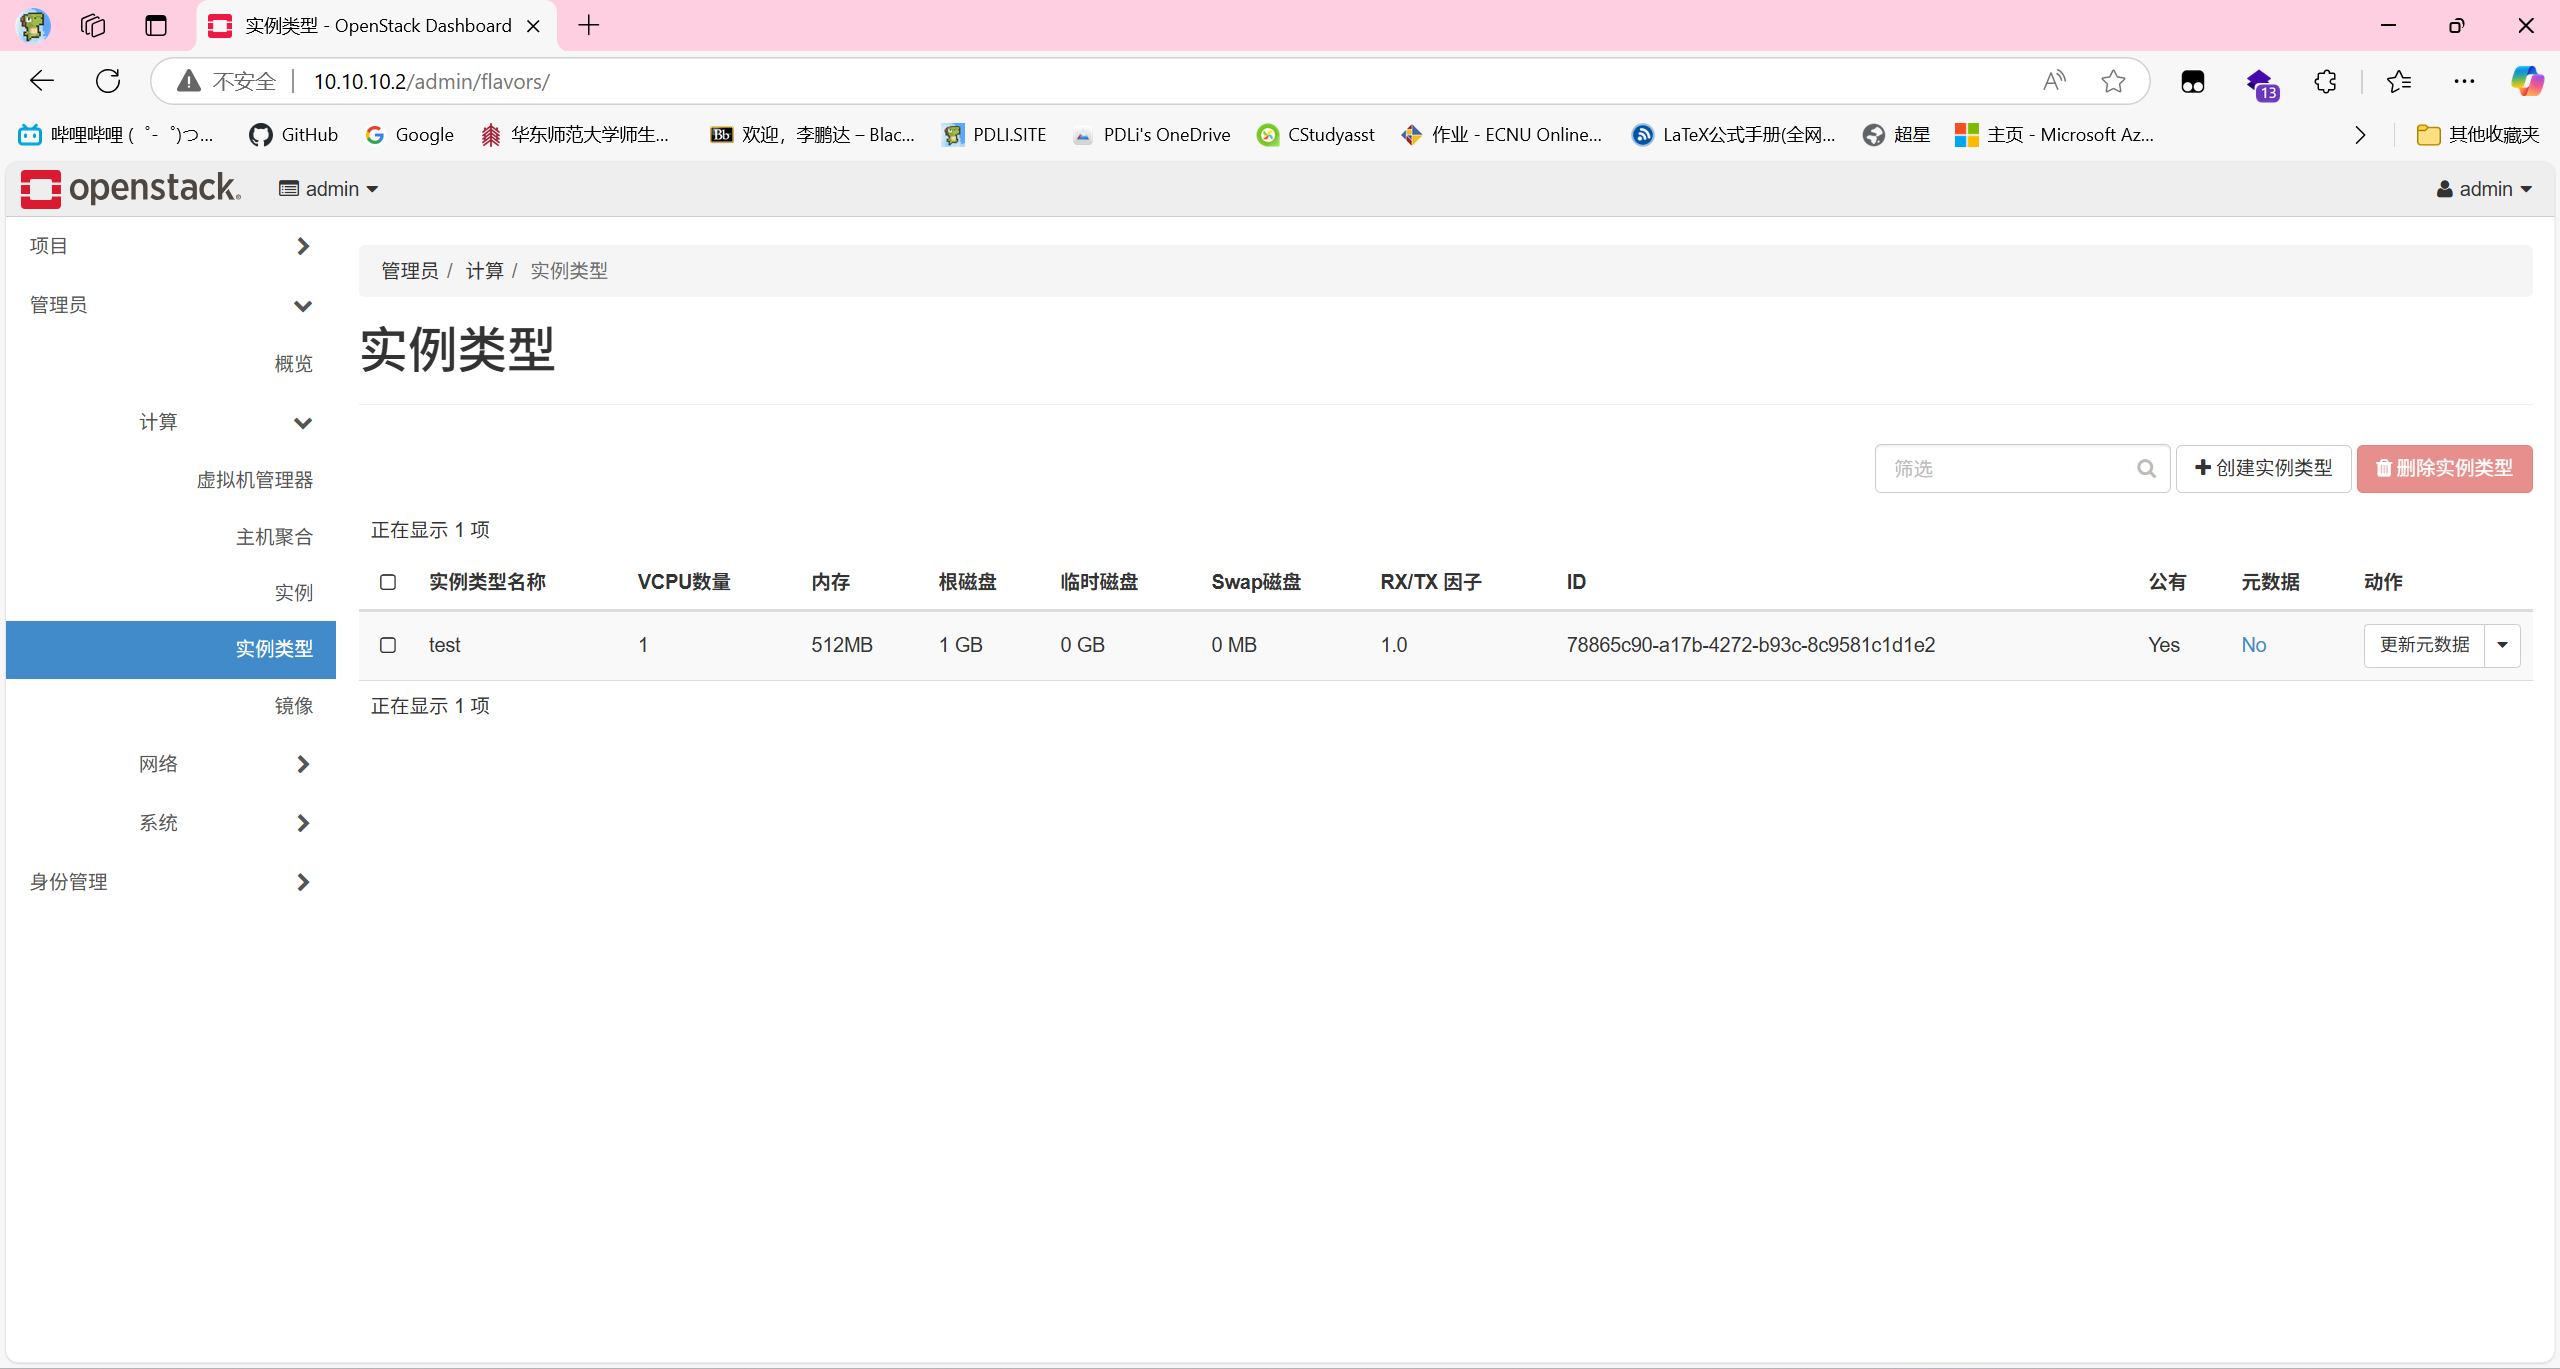
\includegraphics[width=0.8\textwidth]{img/9.2.png}
    \caption{实例类型创建结果}
\end{figure}

\subsubsection{创建网络}

在 OpenStack 中创建一个网络。

\begin{figure}[H]
    \centering
    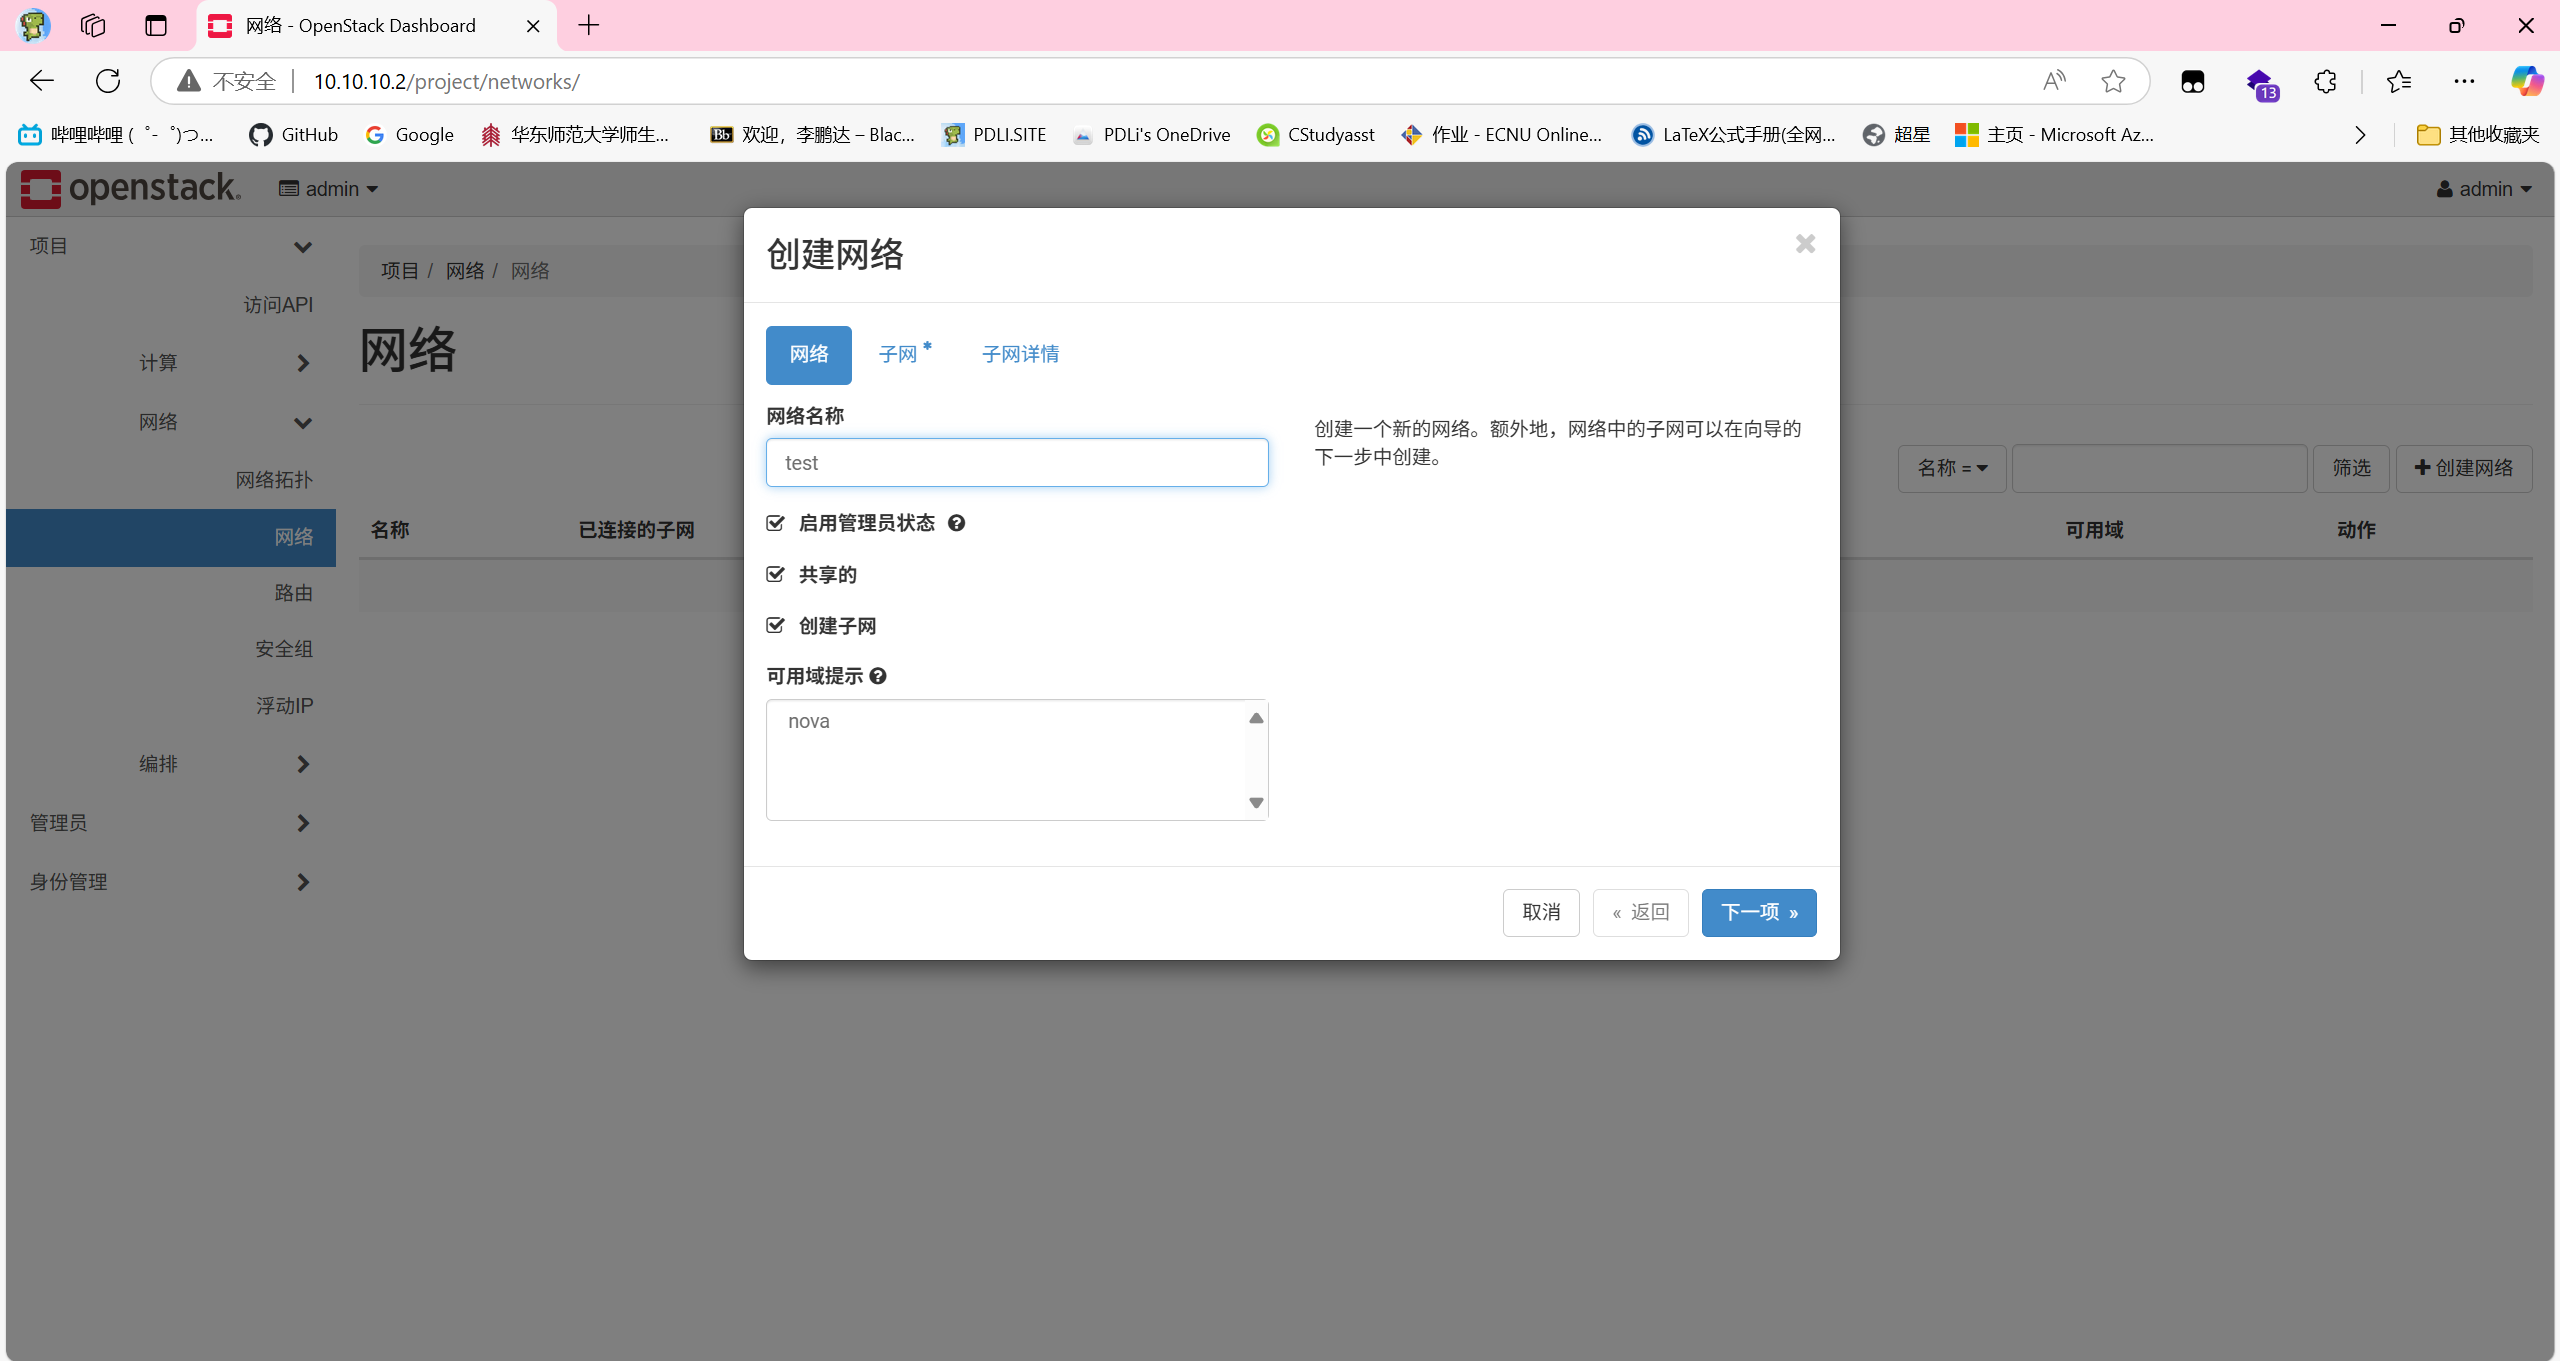
\includegraphics[width=0.8\textwidth]{img/10.1.png}
    \caption{创建网络(1)}
\end{figure}

\begin{figure}[H]
    \centering
    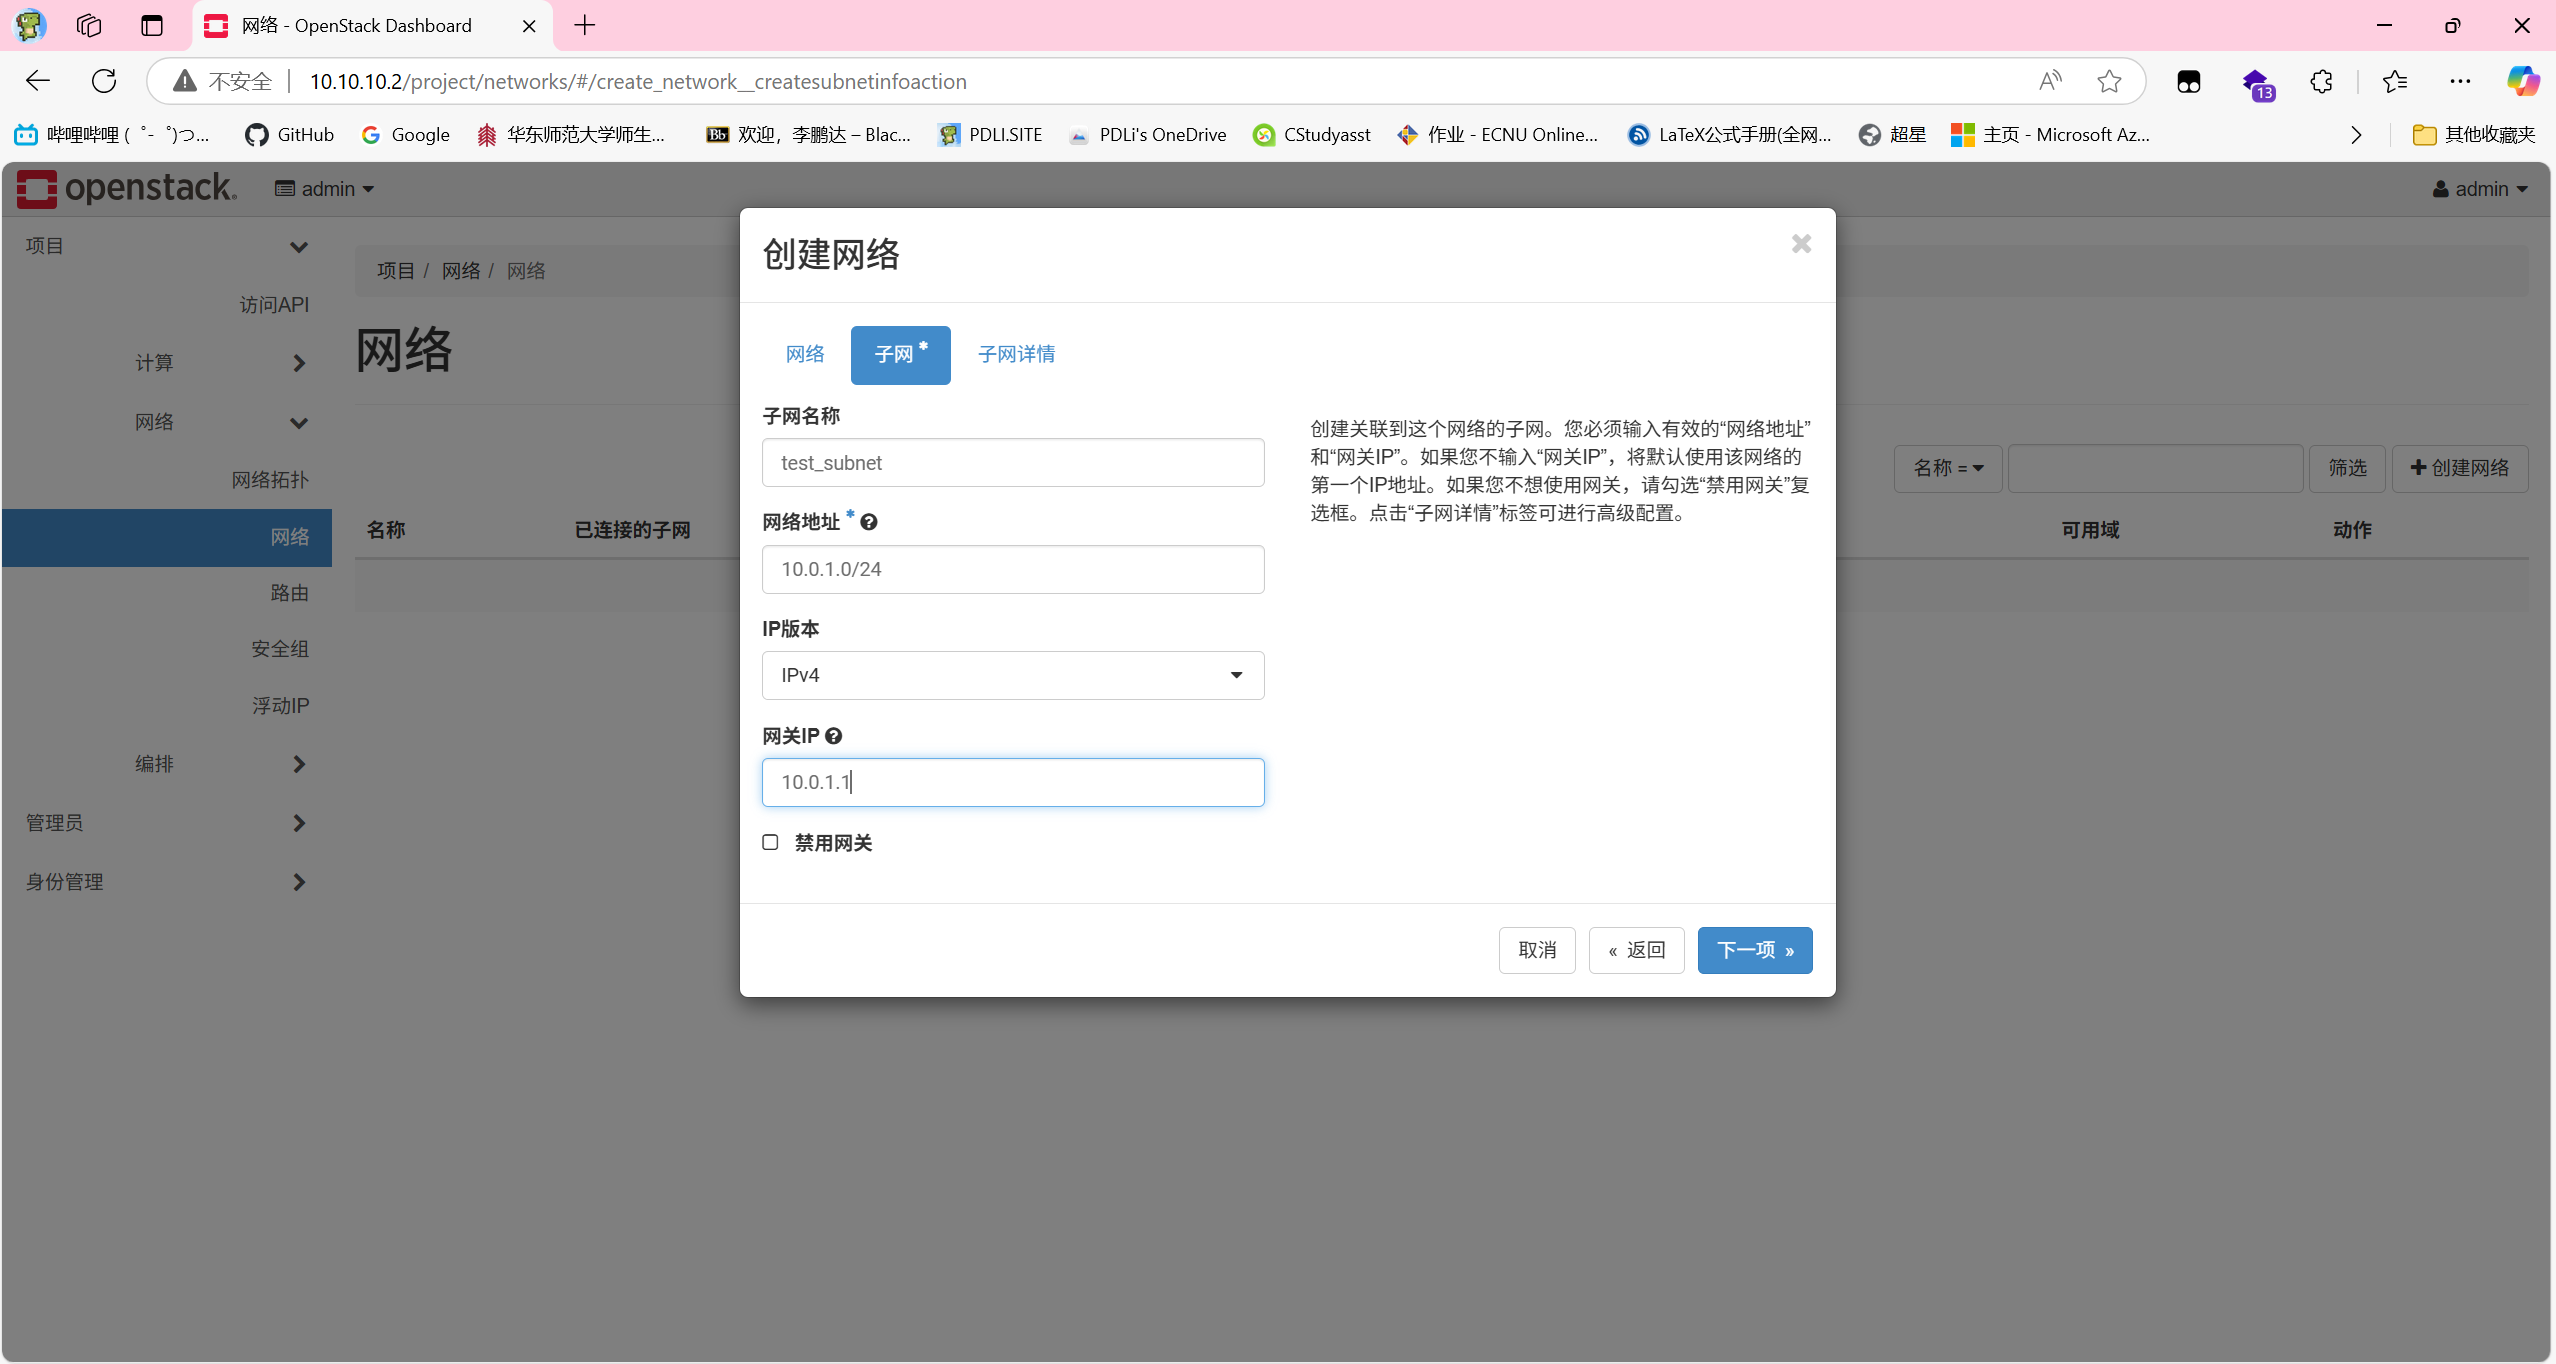
\includegraphics[width=0.8\textwidth]{img/10.2.png}
    \caption{创建网络(2)}
\end{figure}

\begin{figure}[H]
    \centering
    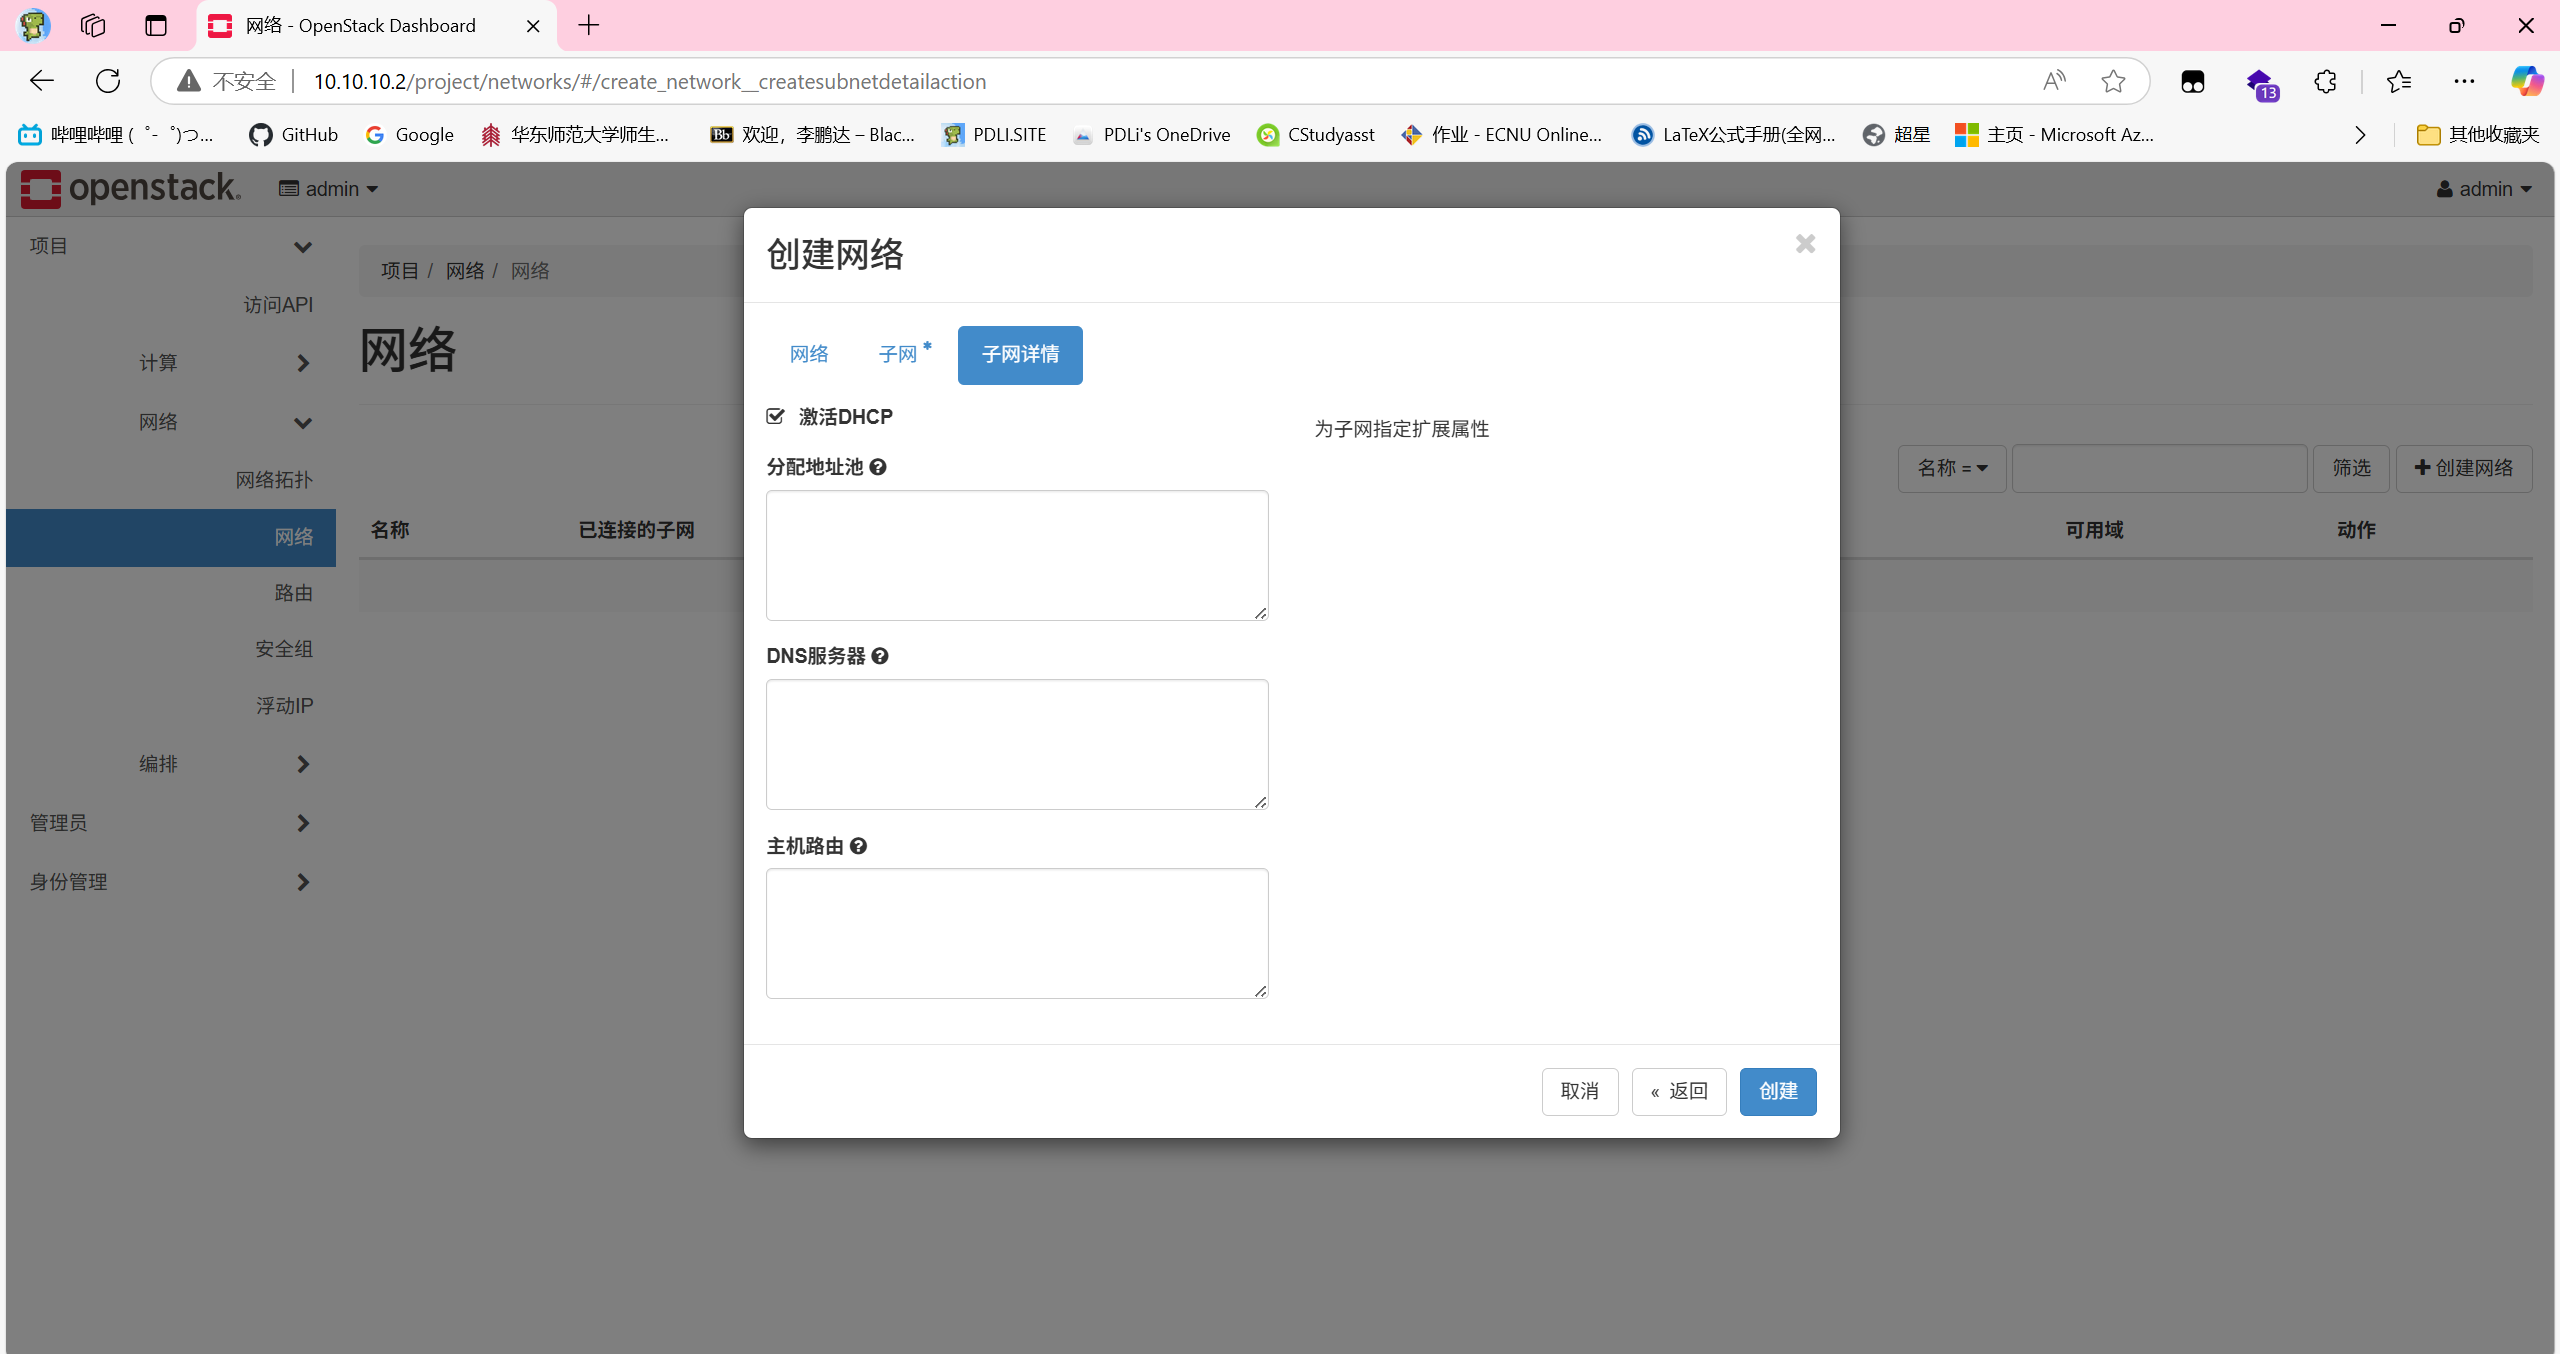
\includegraphics[width=0.8\textwidth]{img/10.3.png}
    \caption{创建网络(3)}
\end{figure}

\begin{figure}[H]
    \centering
    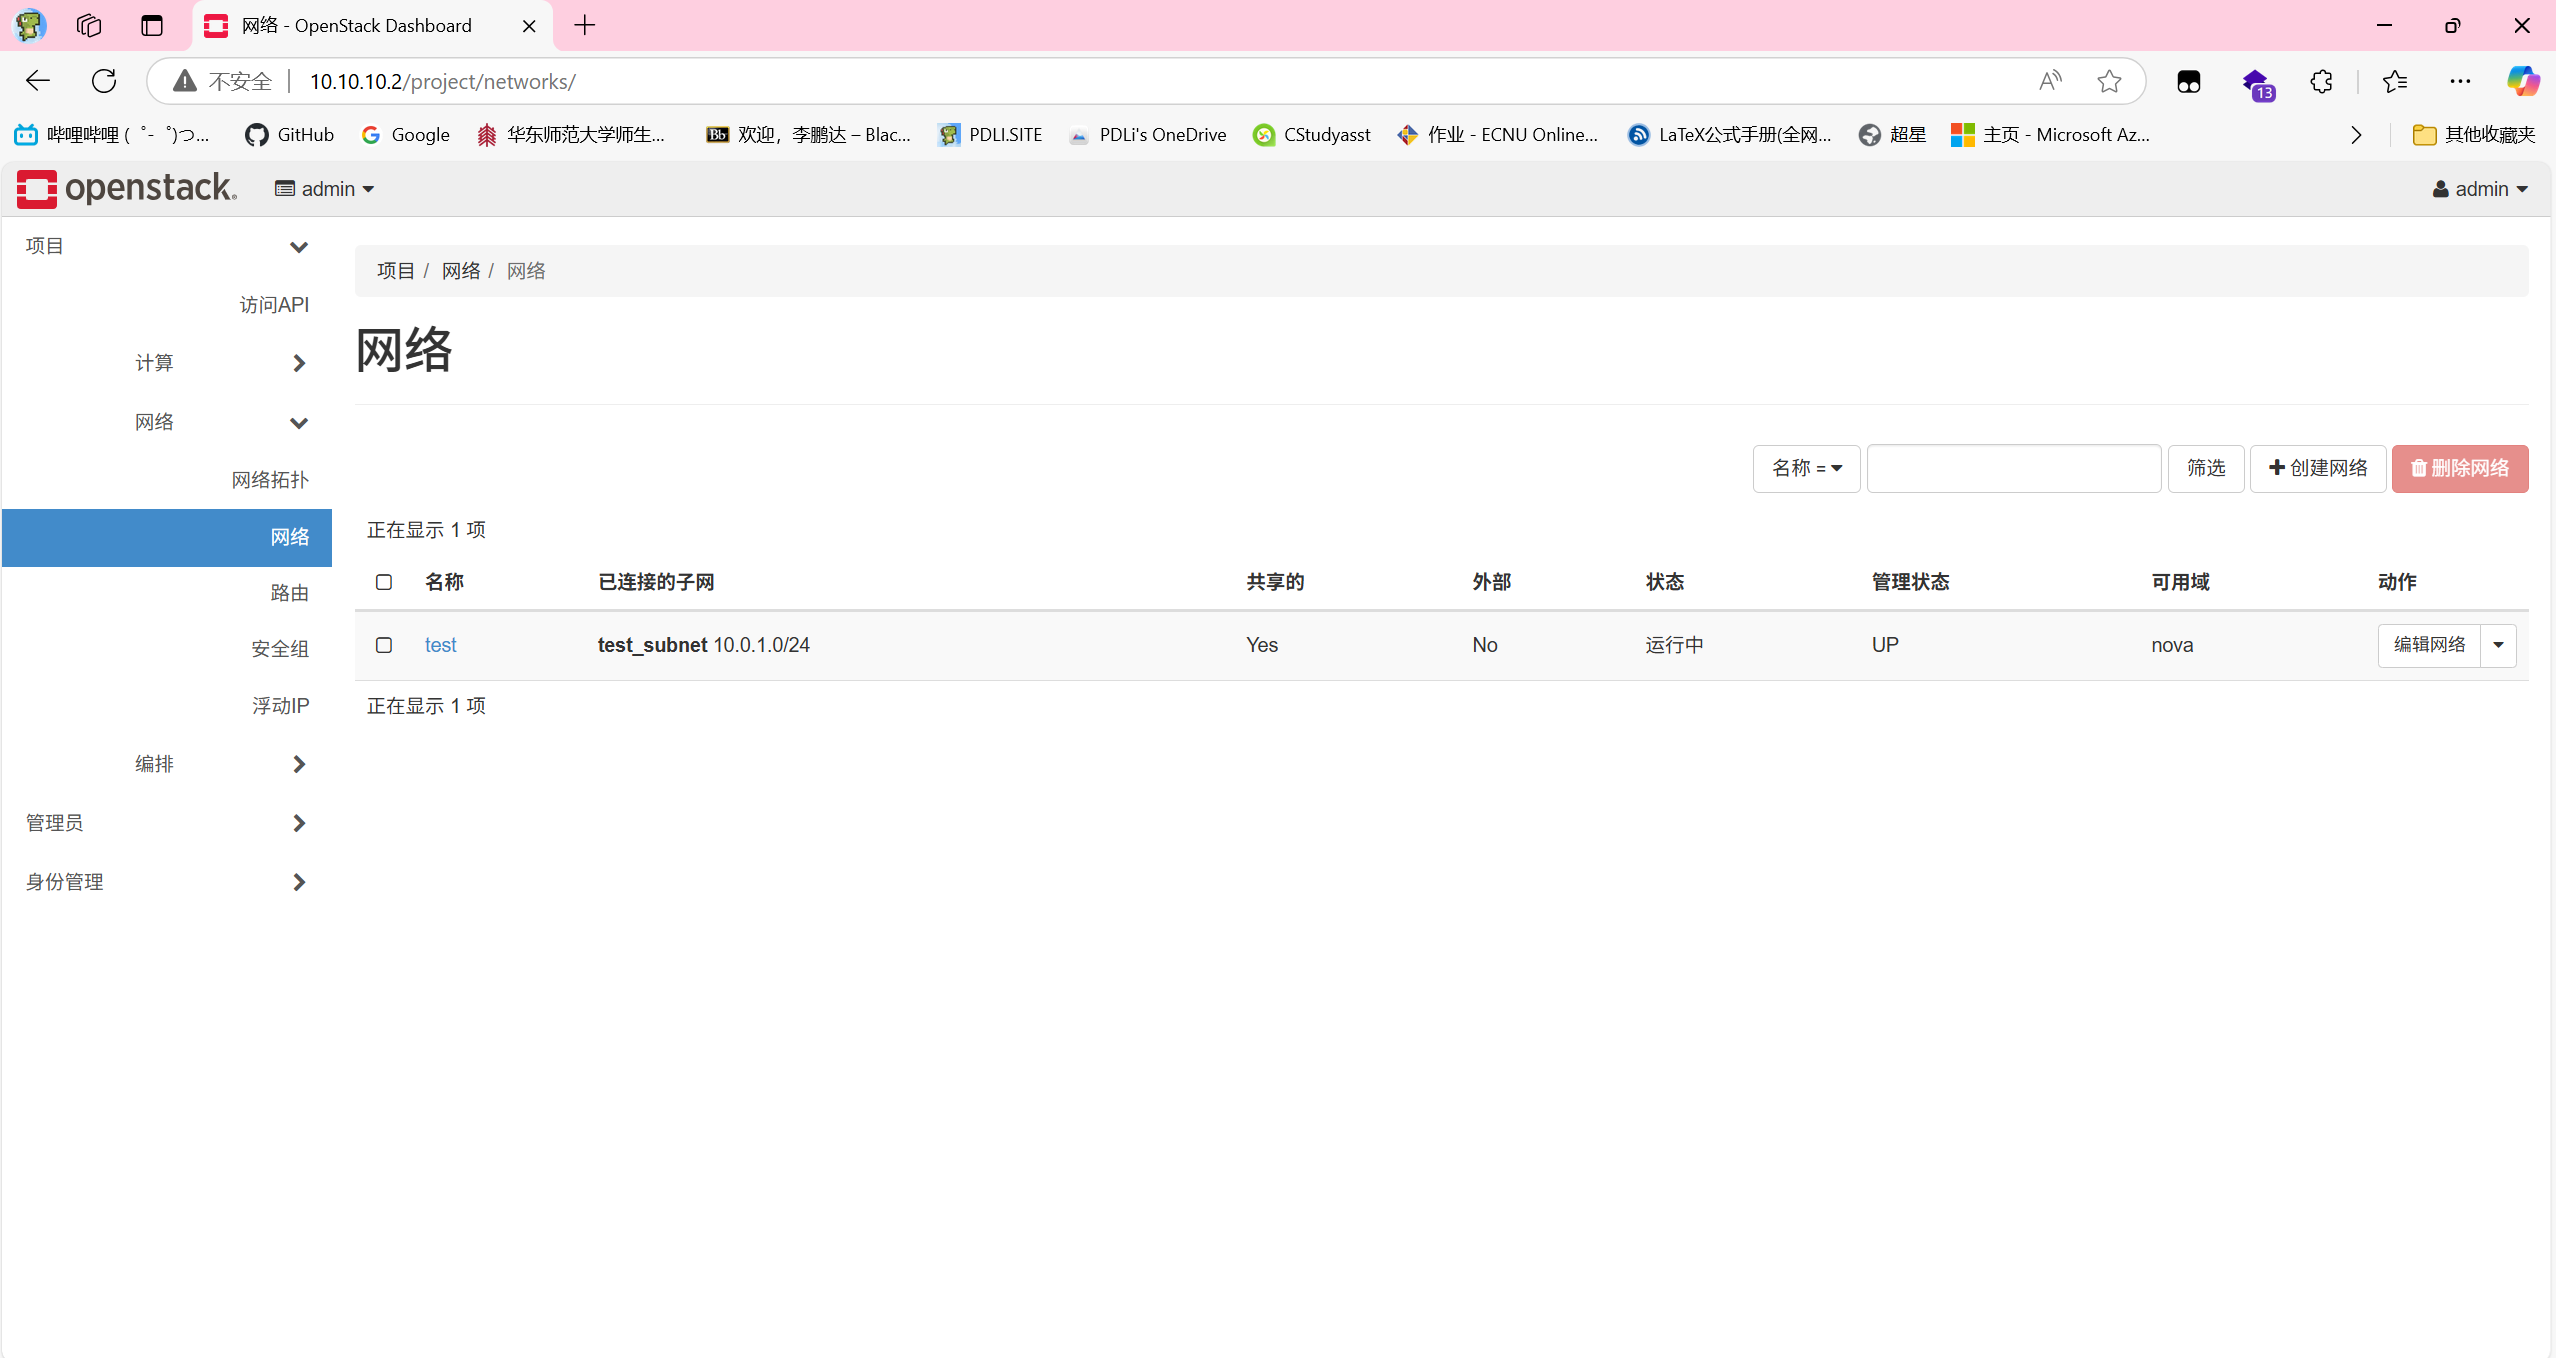
\includegraphics[width=0.8\textwidth]{img/10.4.png}
    \caption{网络创建结果}
\end{figure}

修改配置文件,将 nova-compute 的 \texttt{virt\_type} 改为 \texttt{qemu}。

\begin{lstlisting}[language=bash]
    cd /etc/kolla/nova-compute
    vi nova.conf
\end{lstlisting}

\begin{figure}[H]
    \centering
    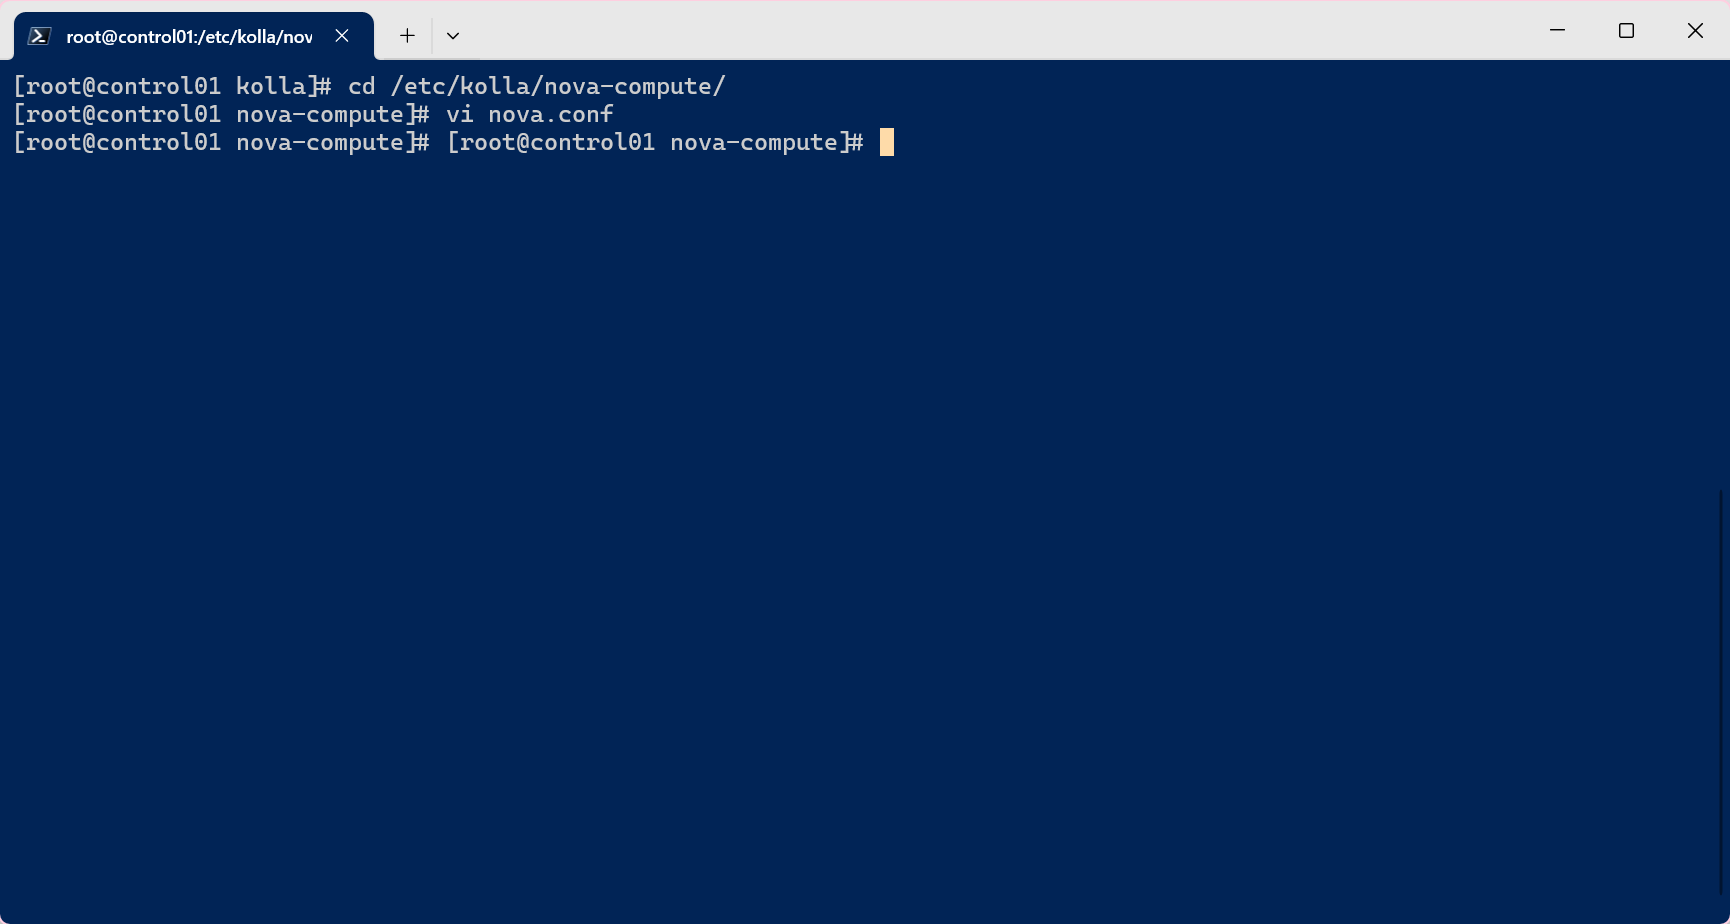
\includegraphics[width=0.8\textwidth]{img/10.5.png}
    \caption{修改配置文件}
\end{figure}

重启 nova-compute 服务,并查看服务状态。

\begin{lstlisting}[language=bash]
    docker restart nova_compute
    docker ps | grep nova_compute
\end{lstlisting}

\begin{figure}[H]
    \centering
    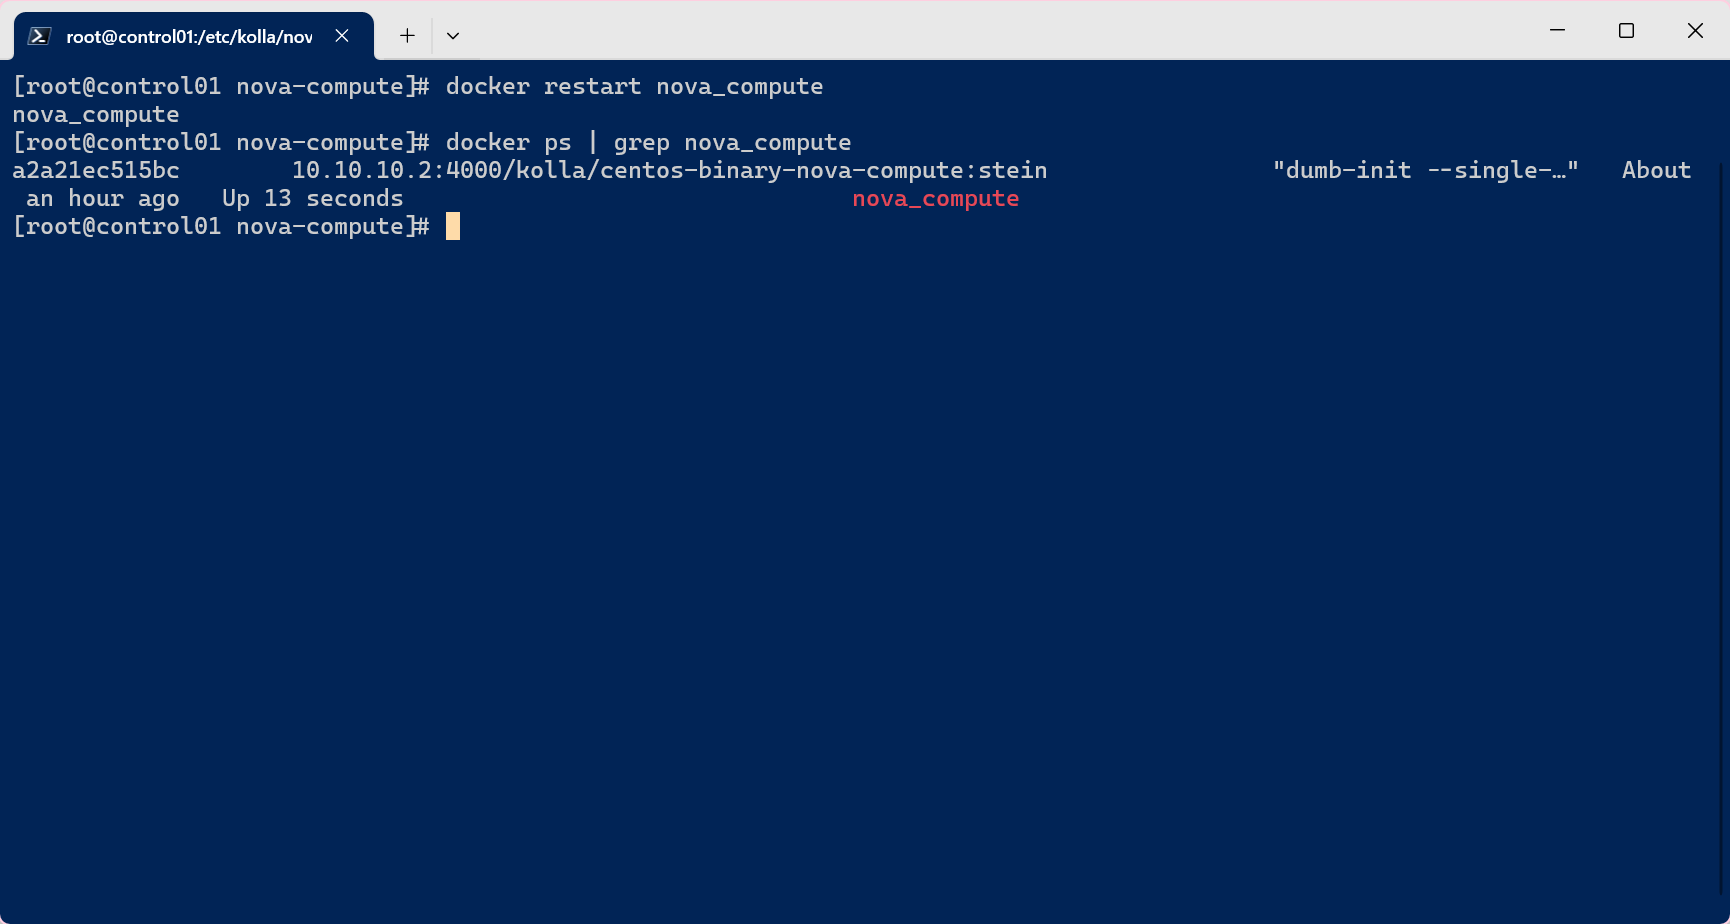
\includegraphics[width=0.8\textwidth]{img/10.6.png}
    \caption{重启服务并查看服务状态}
\end{figure}

\subsubsection{创建实例}

在 OpenStack 中创建一个实例。

\begin{figure}[H]
    \centering
    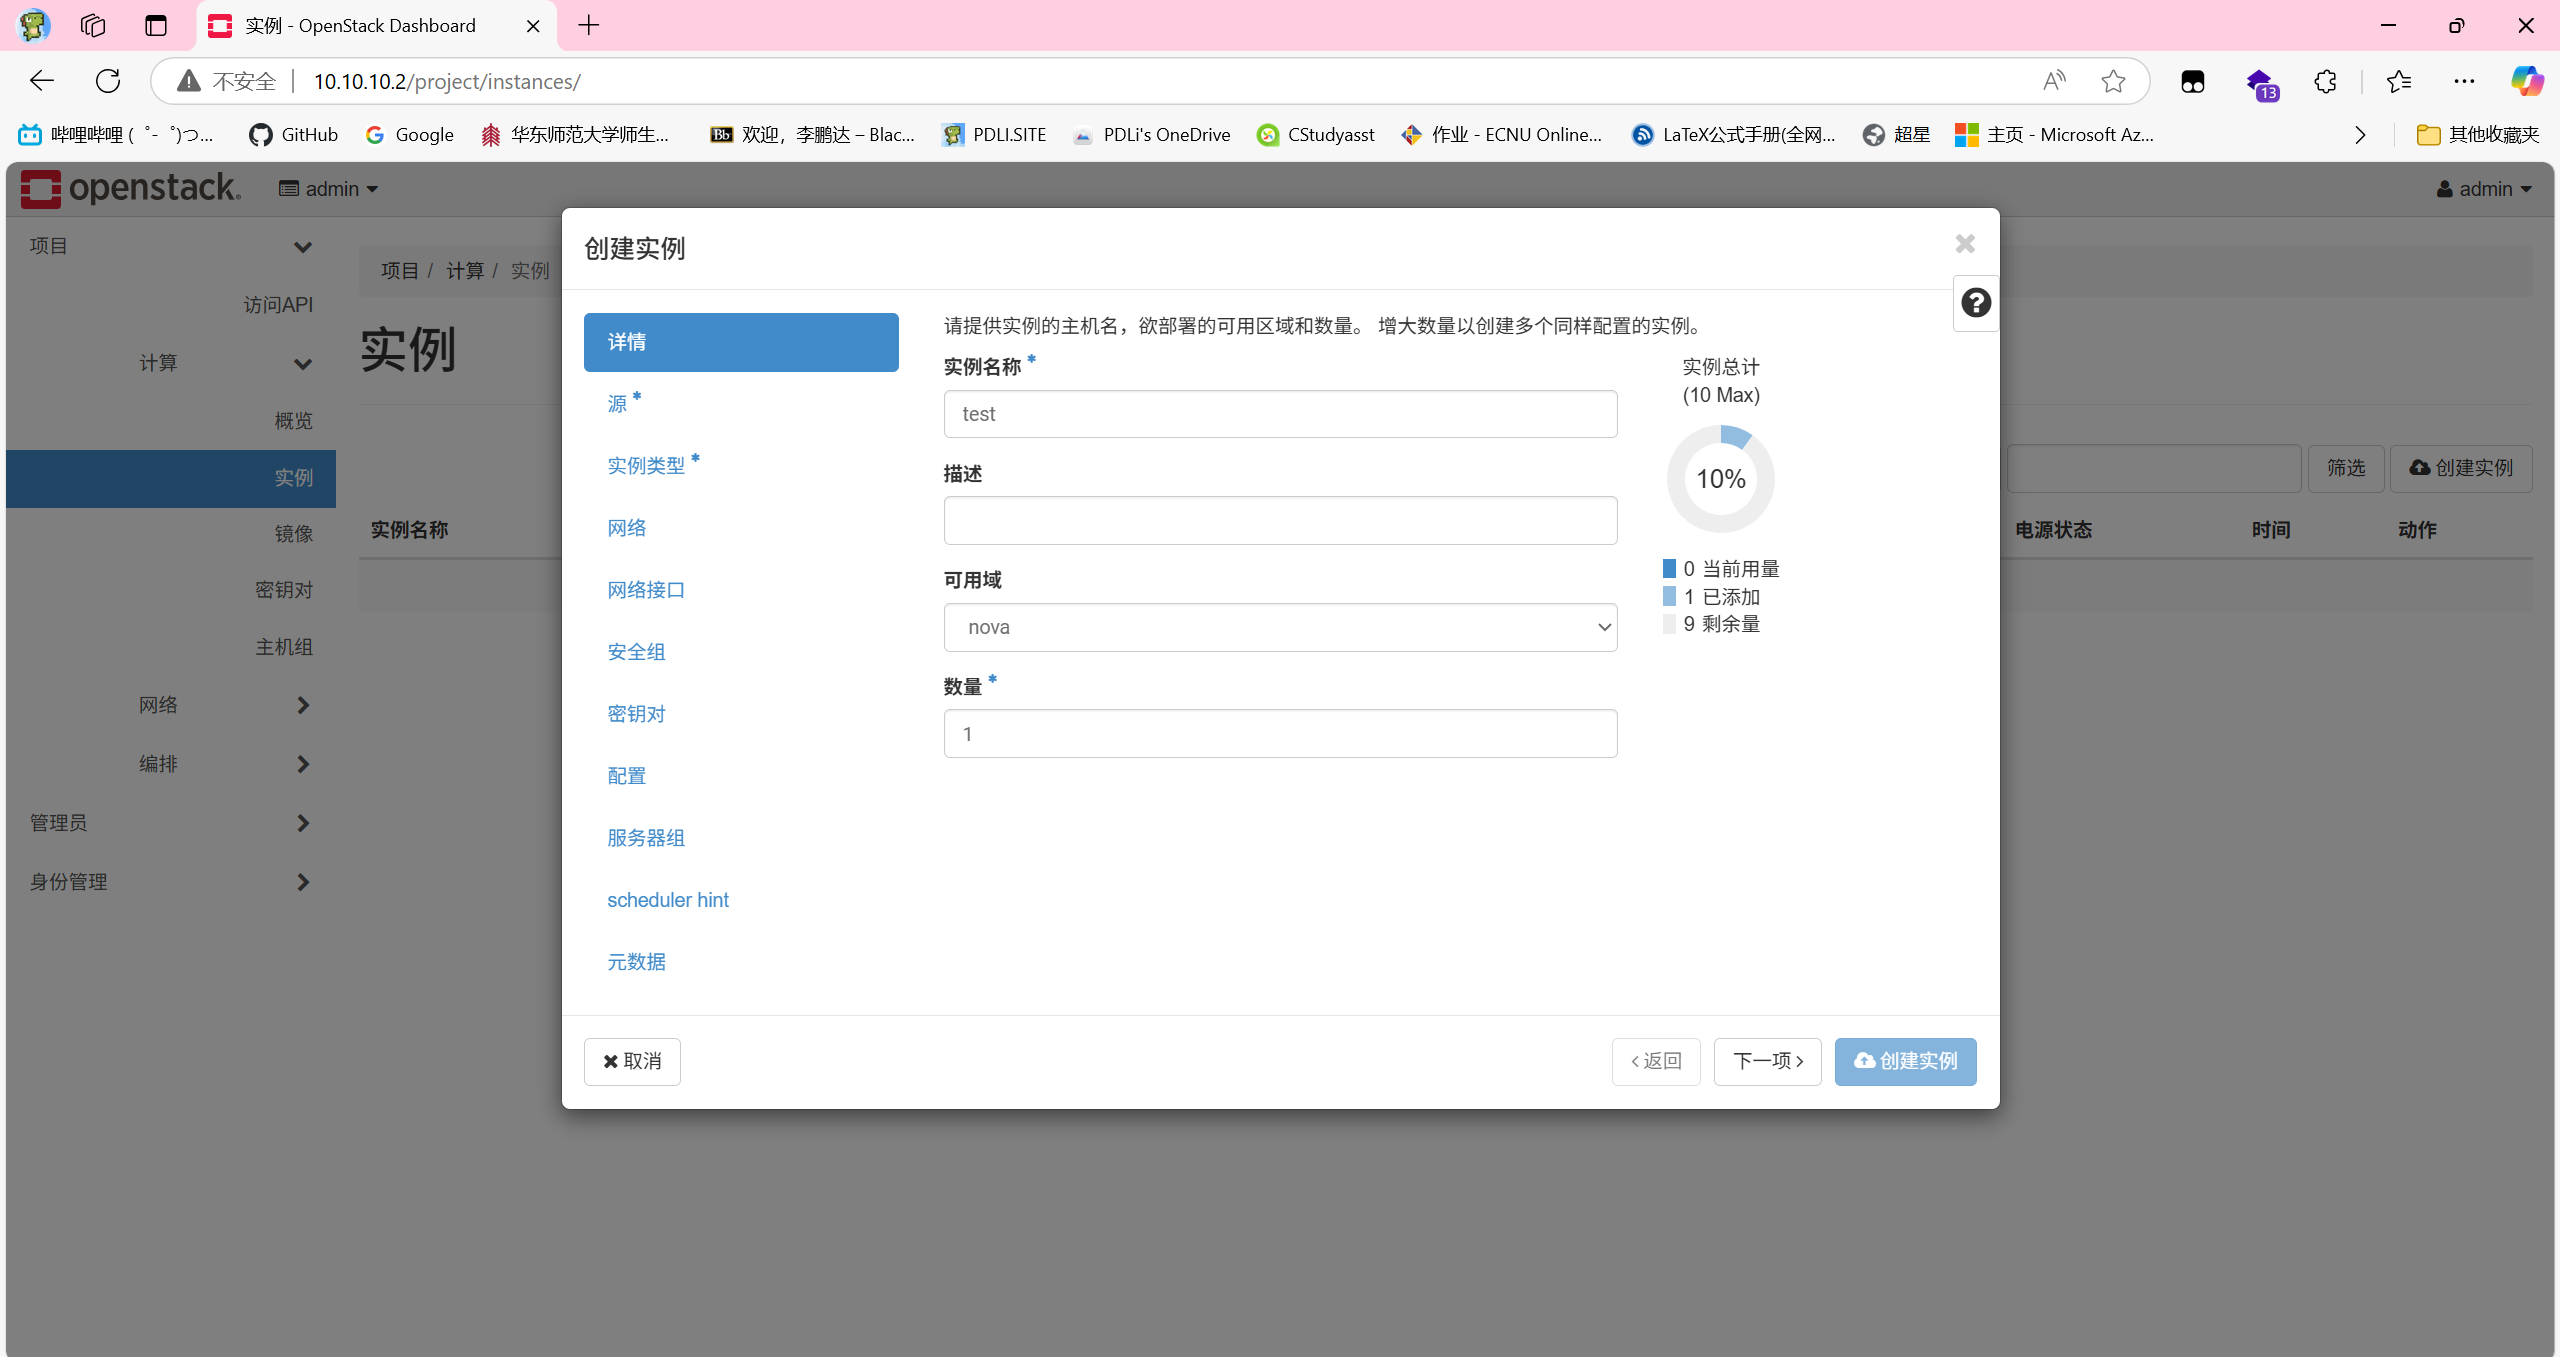
\includegraphics[width=0.8\textwidth]{img/11.1.png}
    \caption{创建实例(1)}
\end{figure}

\begin{figure}[H]
    \centering
    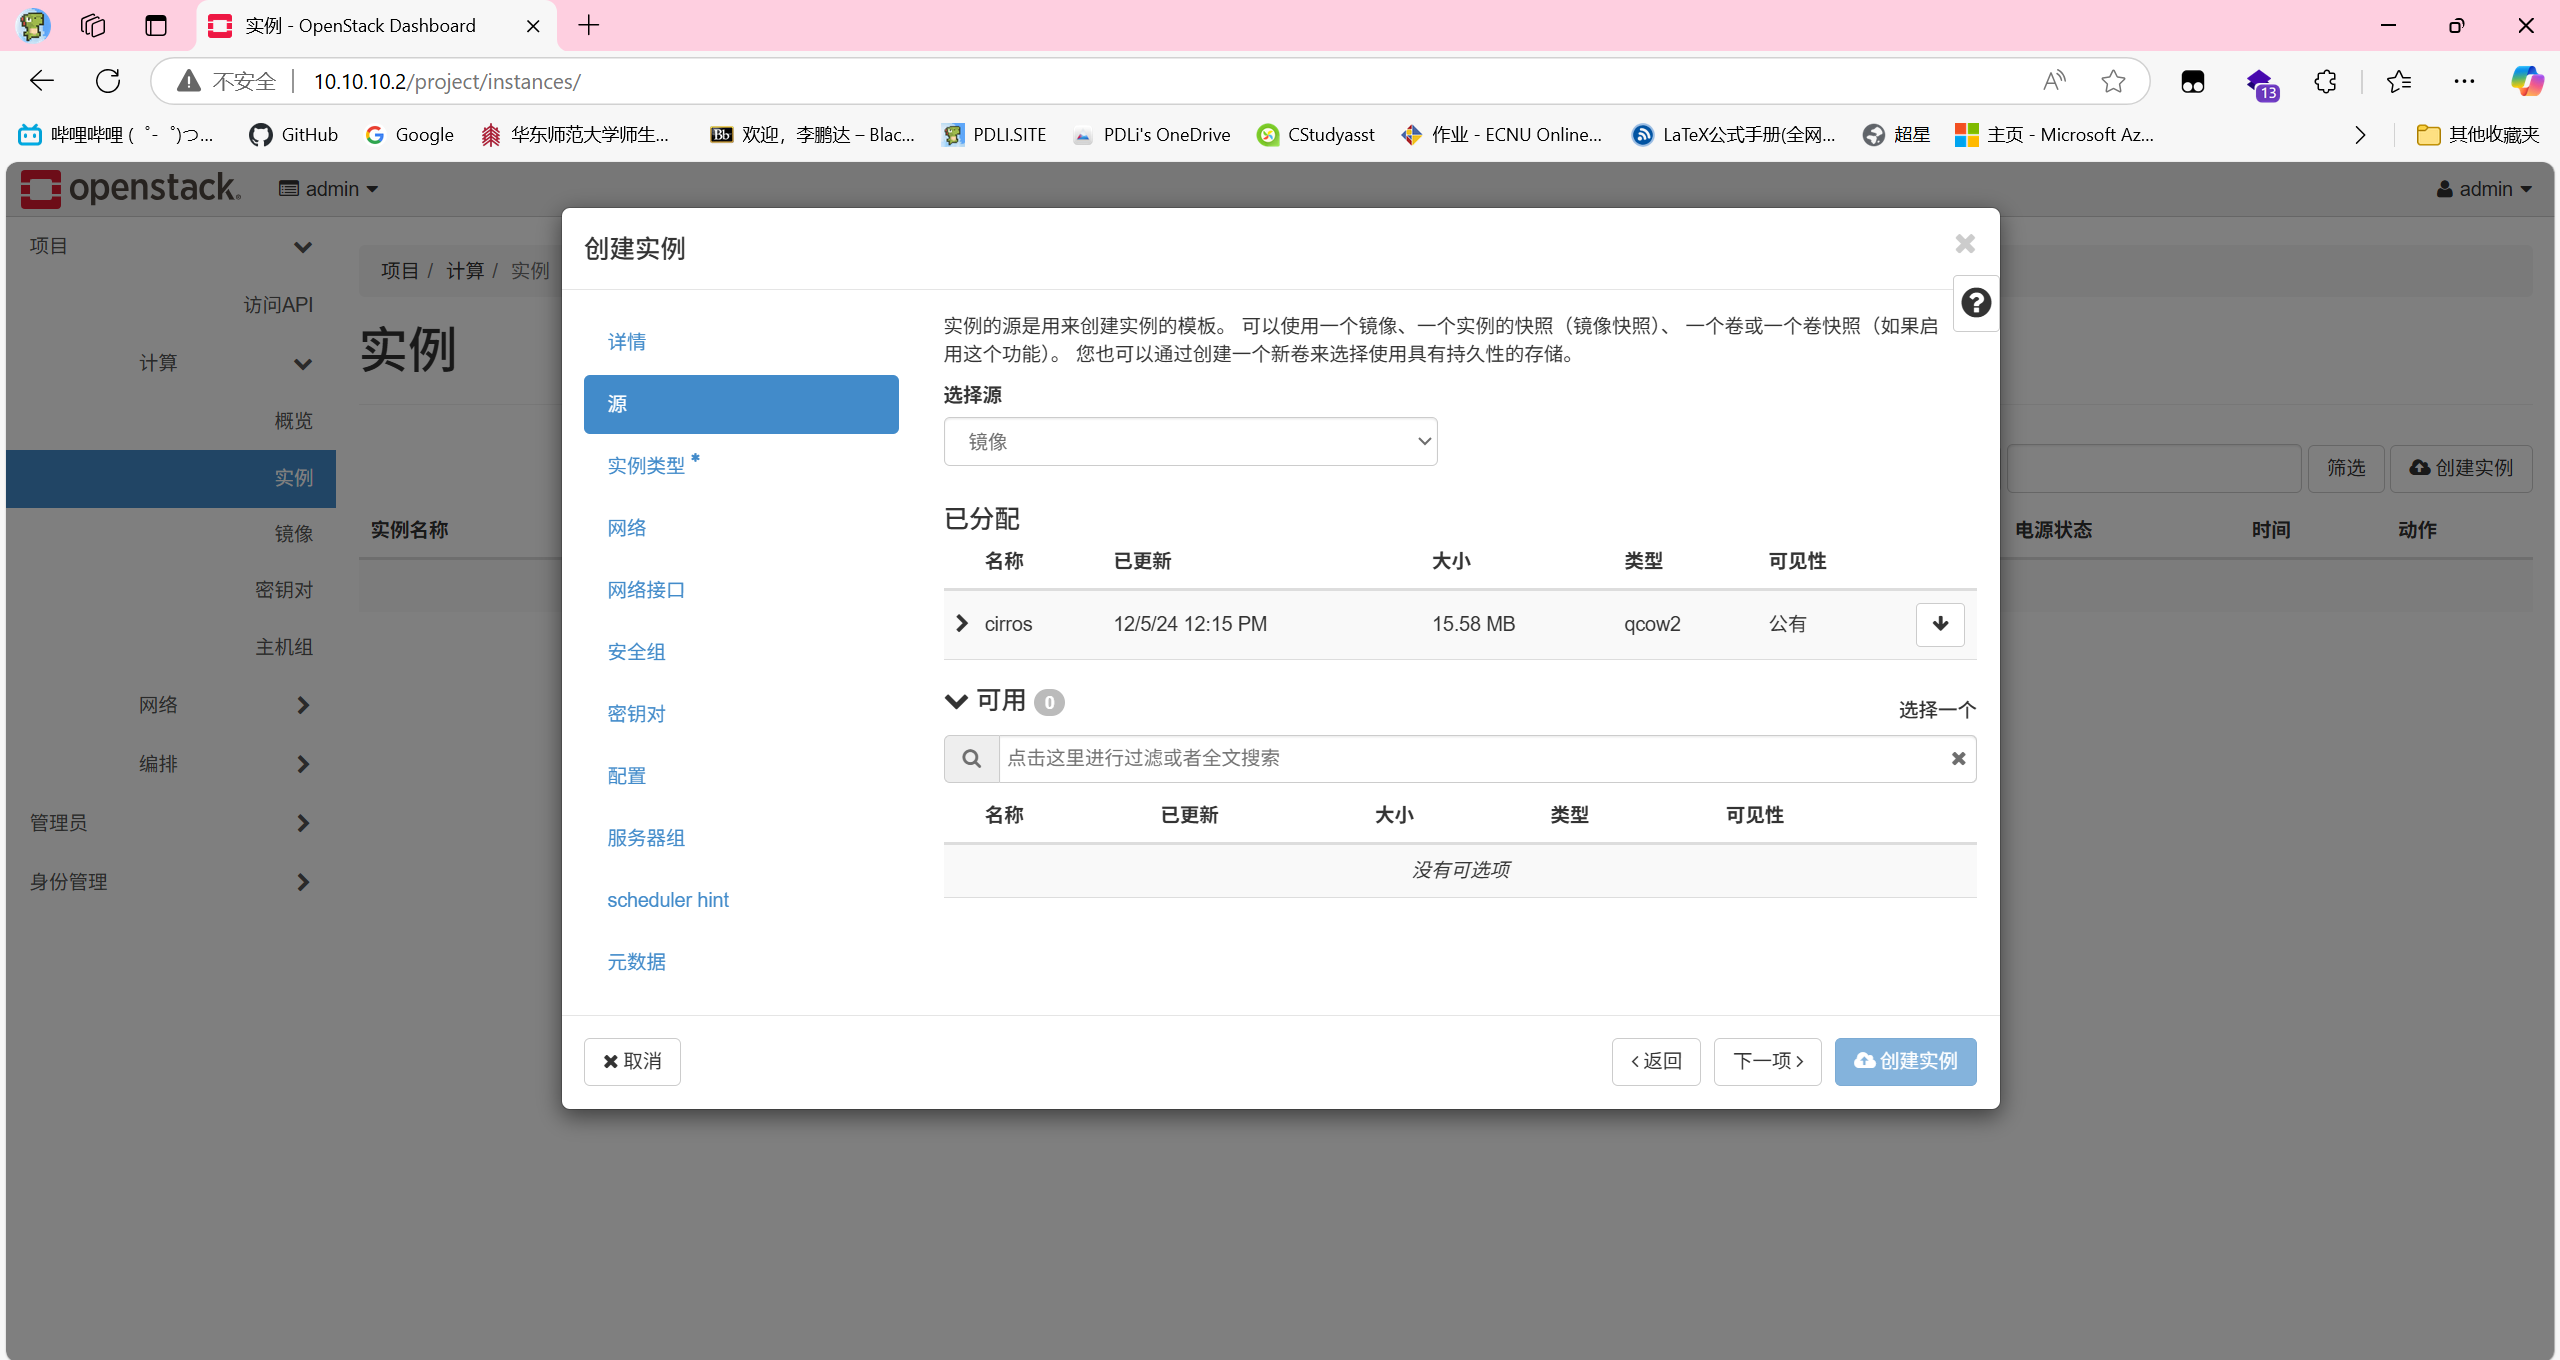
\includegraphics[width=0.8\textwidth]{img/11.2.png}
    \caption{创建实例(2)}
\end{figure}

\begin{figure}[H]
    \centering
    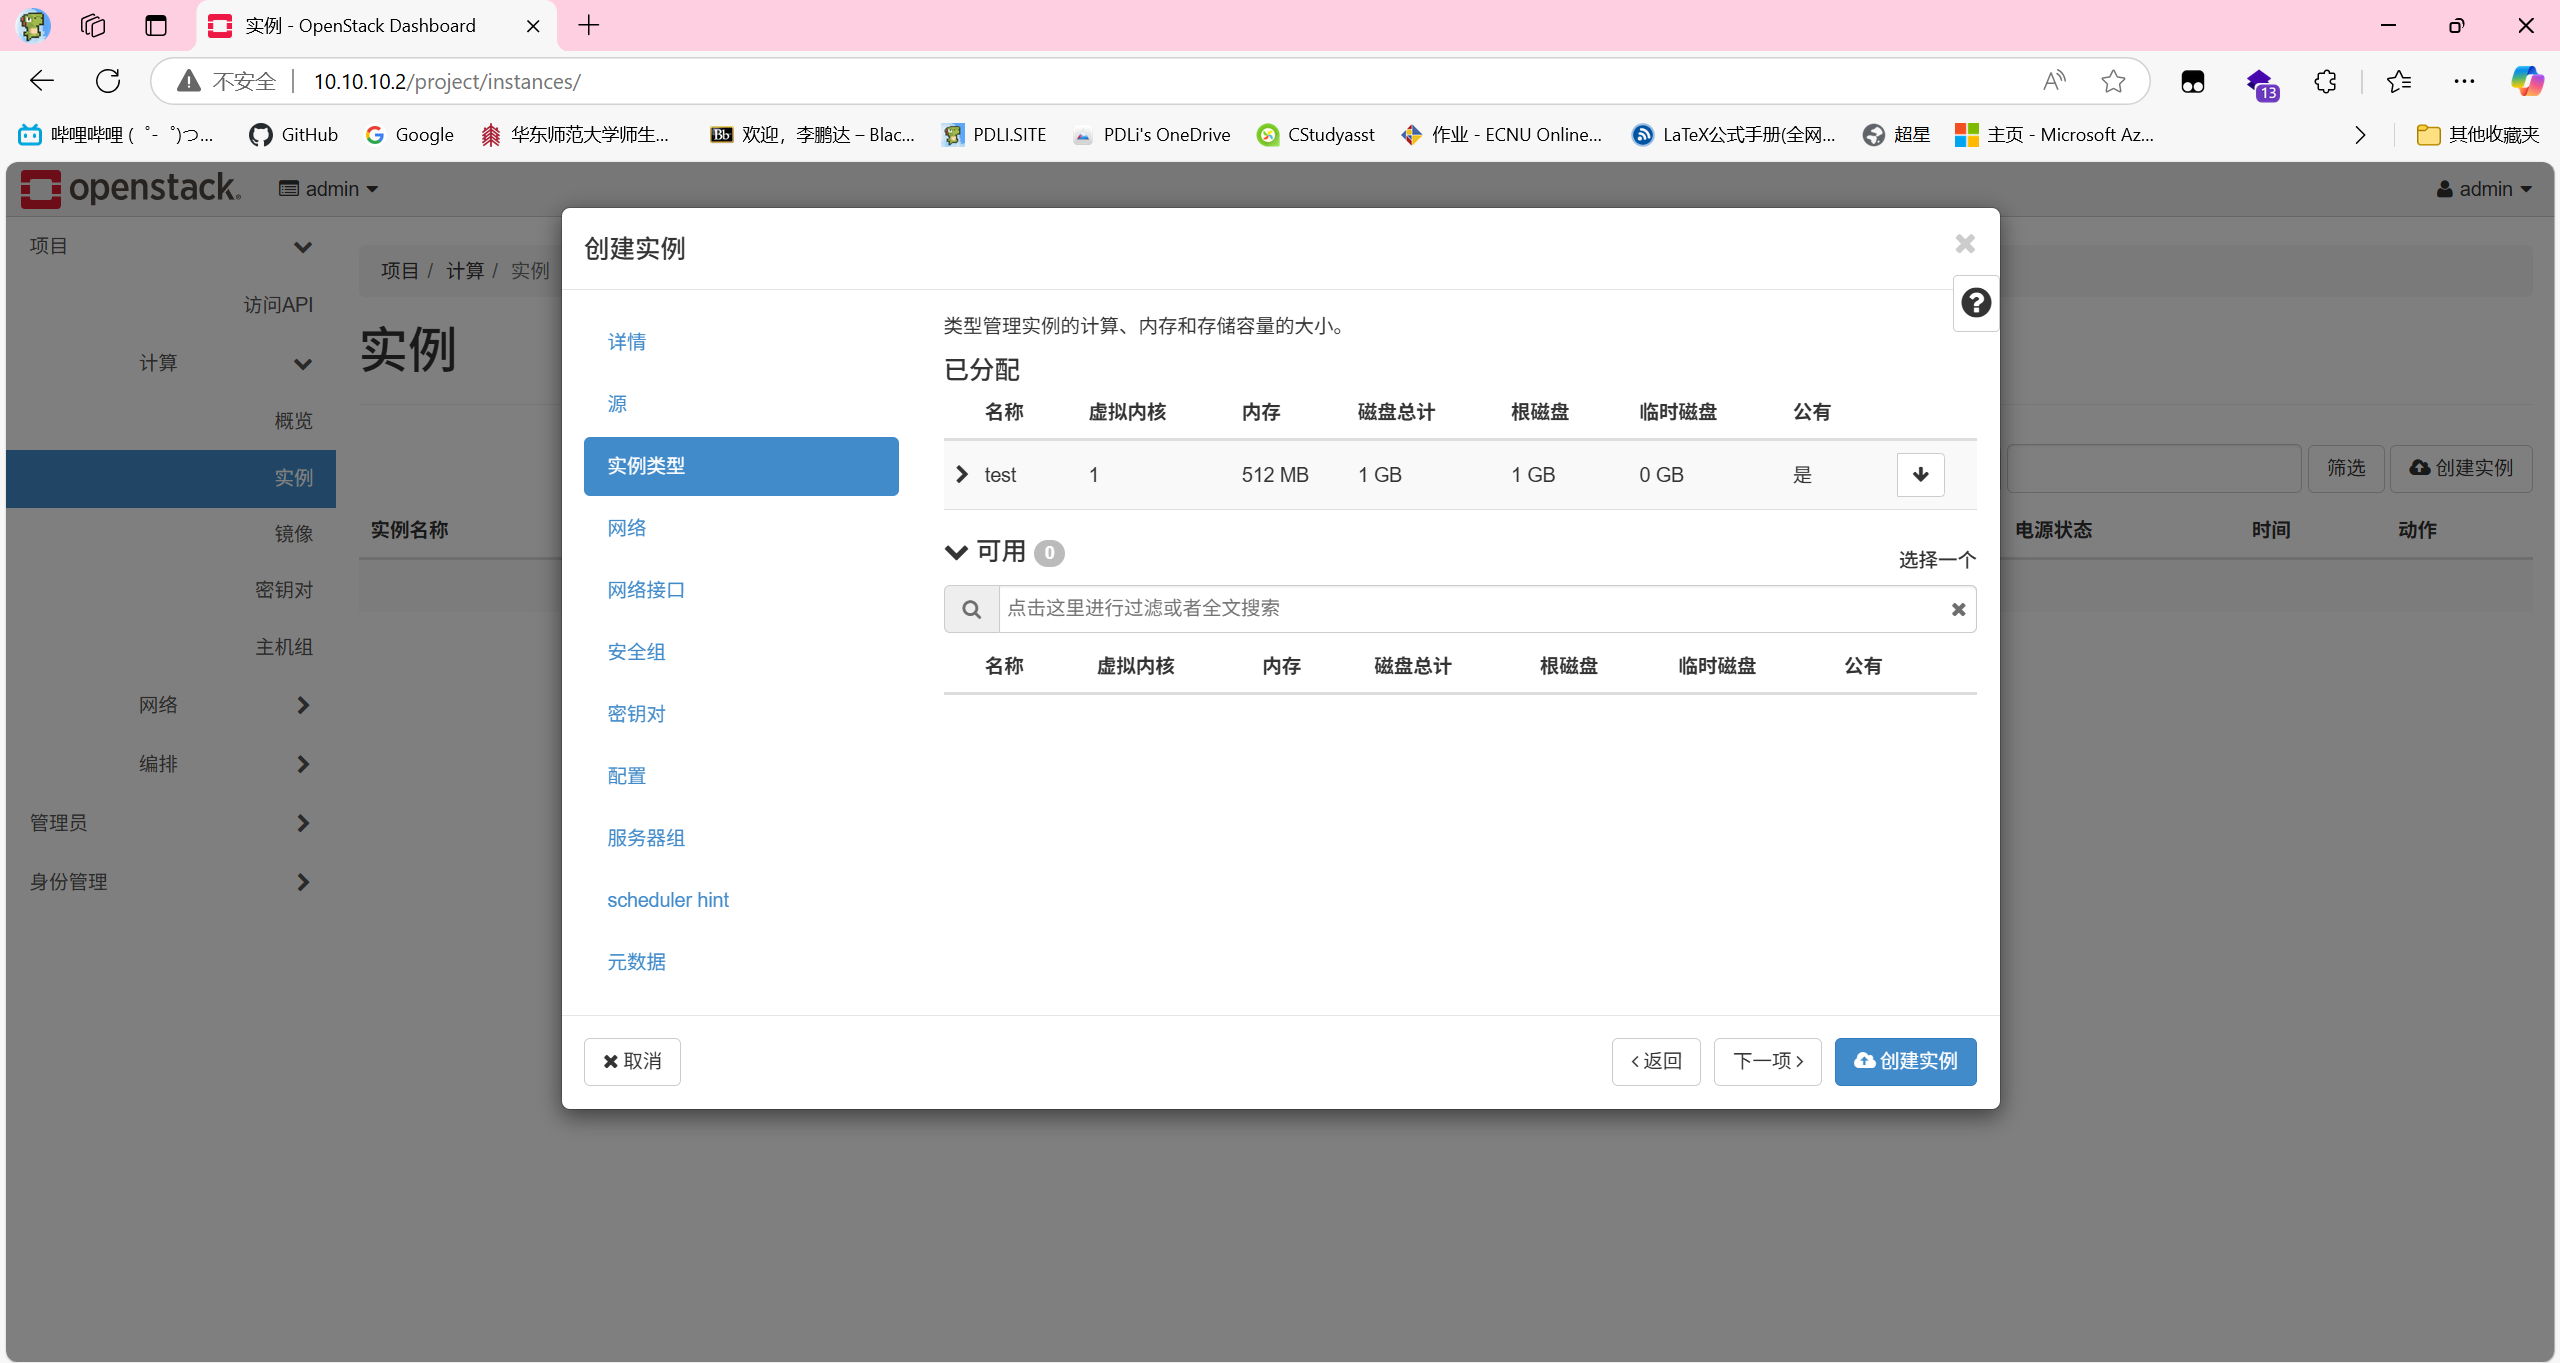
\includegraphics[width=0.8\textwidth]{img/11.3.png}
    \caption{创建实例(3)}
\end{figure}

\begin{figure}[H]
    \centering
    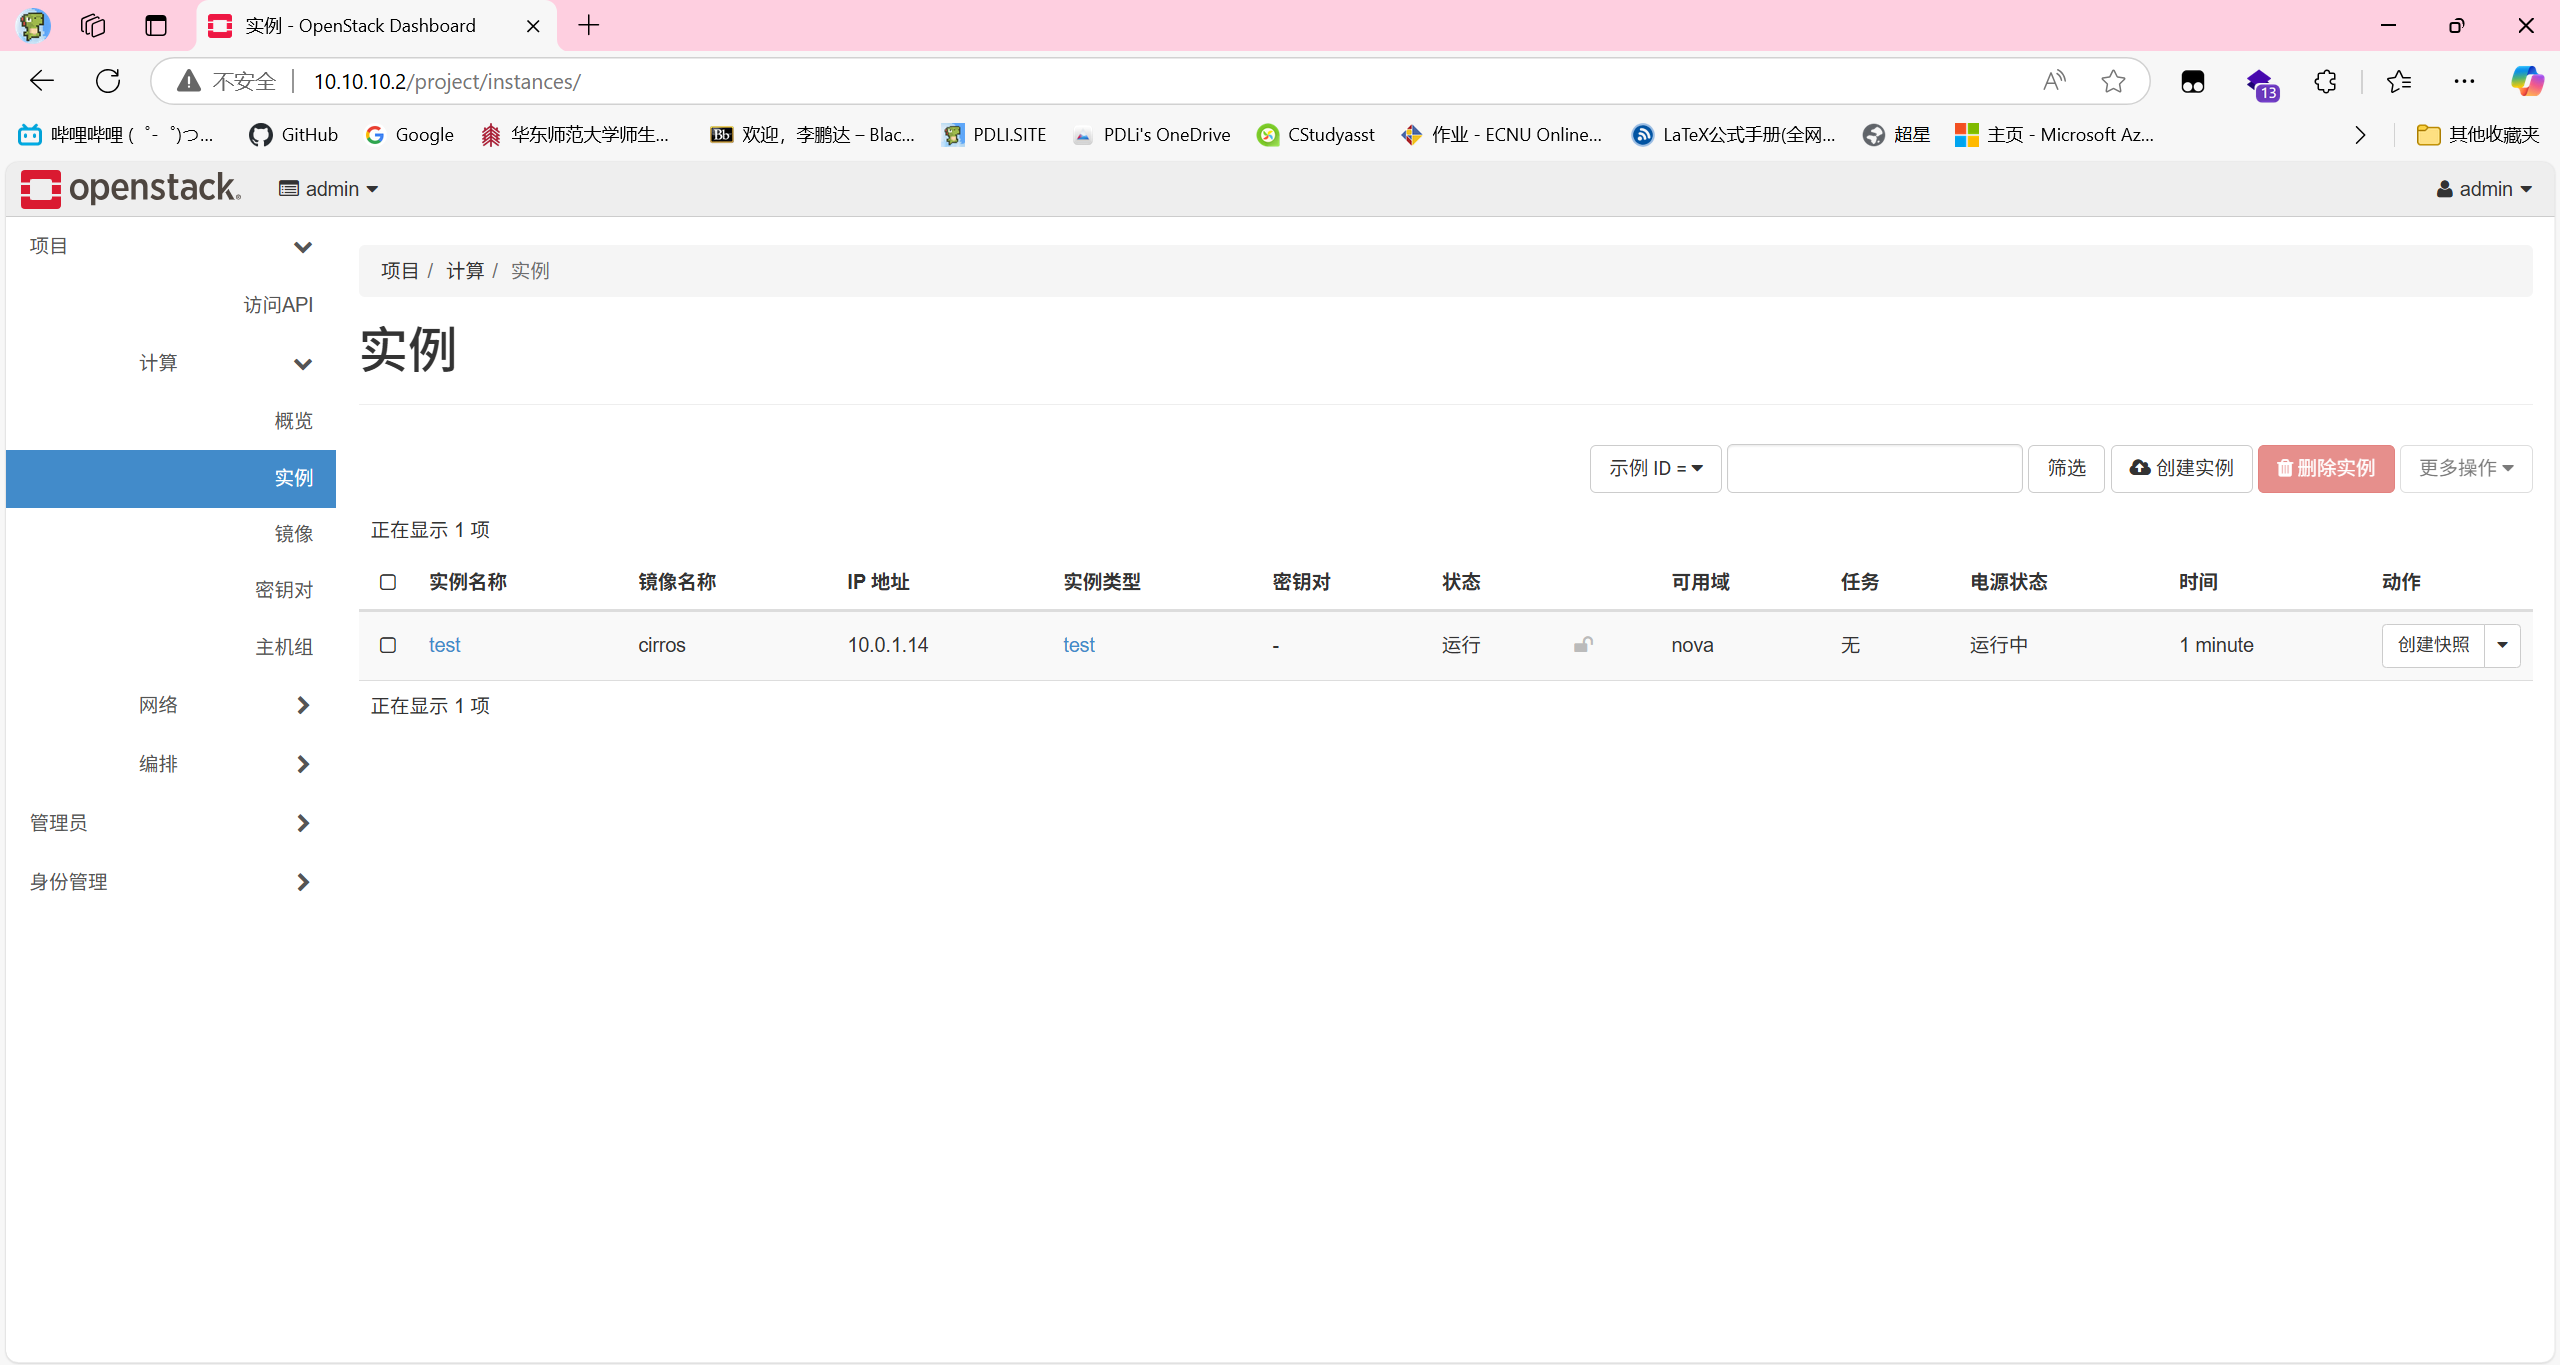
\includegraphics[width=0.8\textwidth]{img/11.4.png}
    \caption{实例创建结果}
\end{figure}


\section{实验结果}

\subsection{openstack服务列表}

\begin{figure}[H]
    \centering
    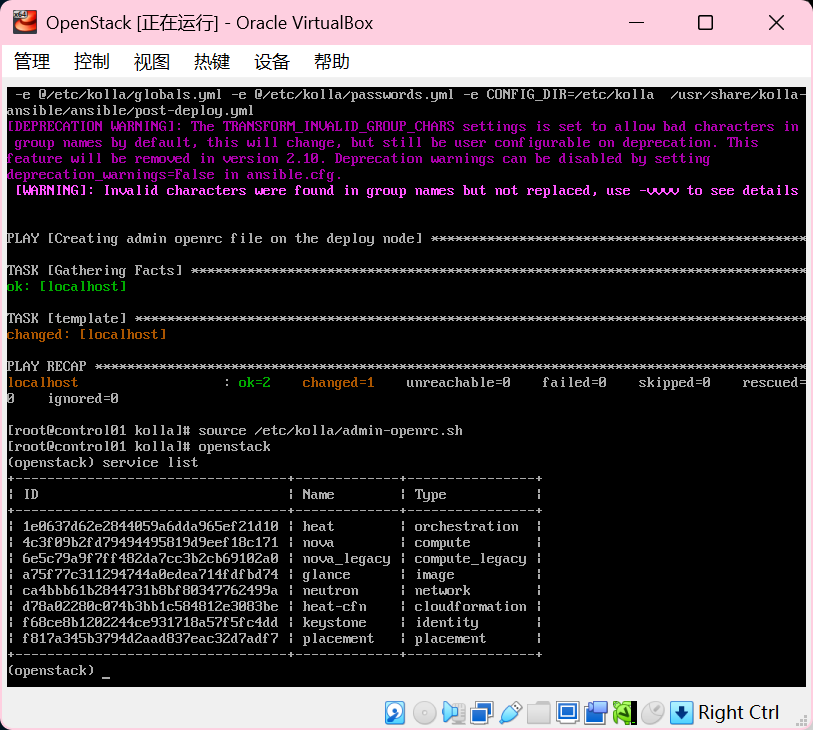
\includegraphics[width=0.55\textwidth]{img/7.6.png}
    \caption{openstack服务列表}
\end{figure}

\subsection{OpenStack控制台}

\begin{figure}[H]
    \centering
    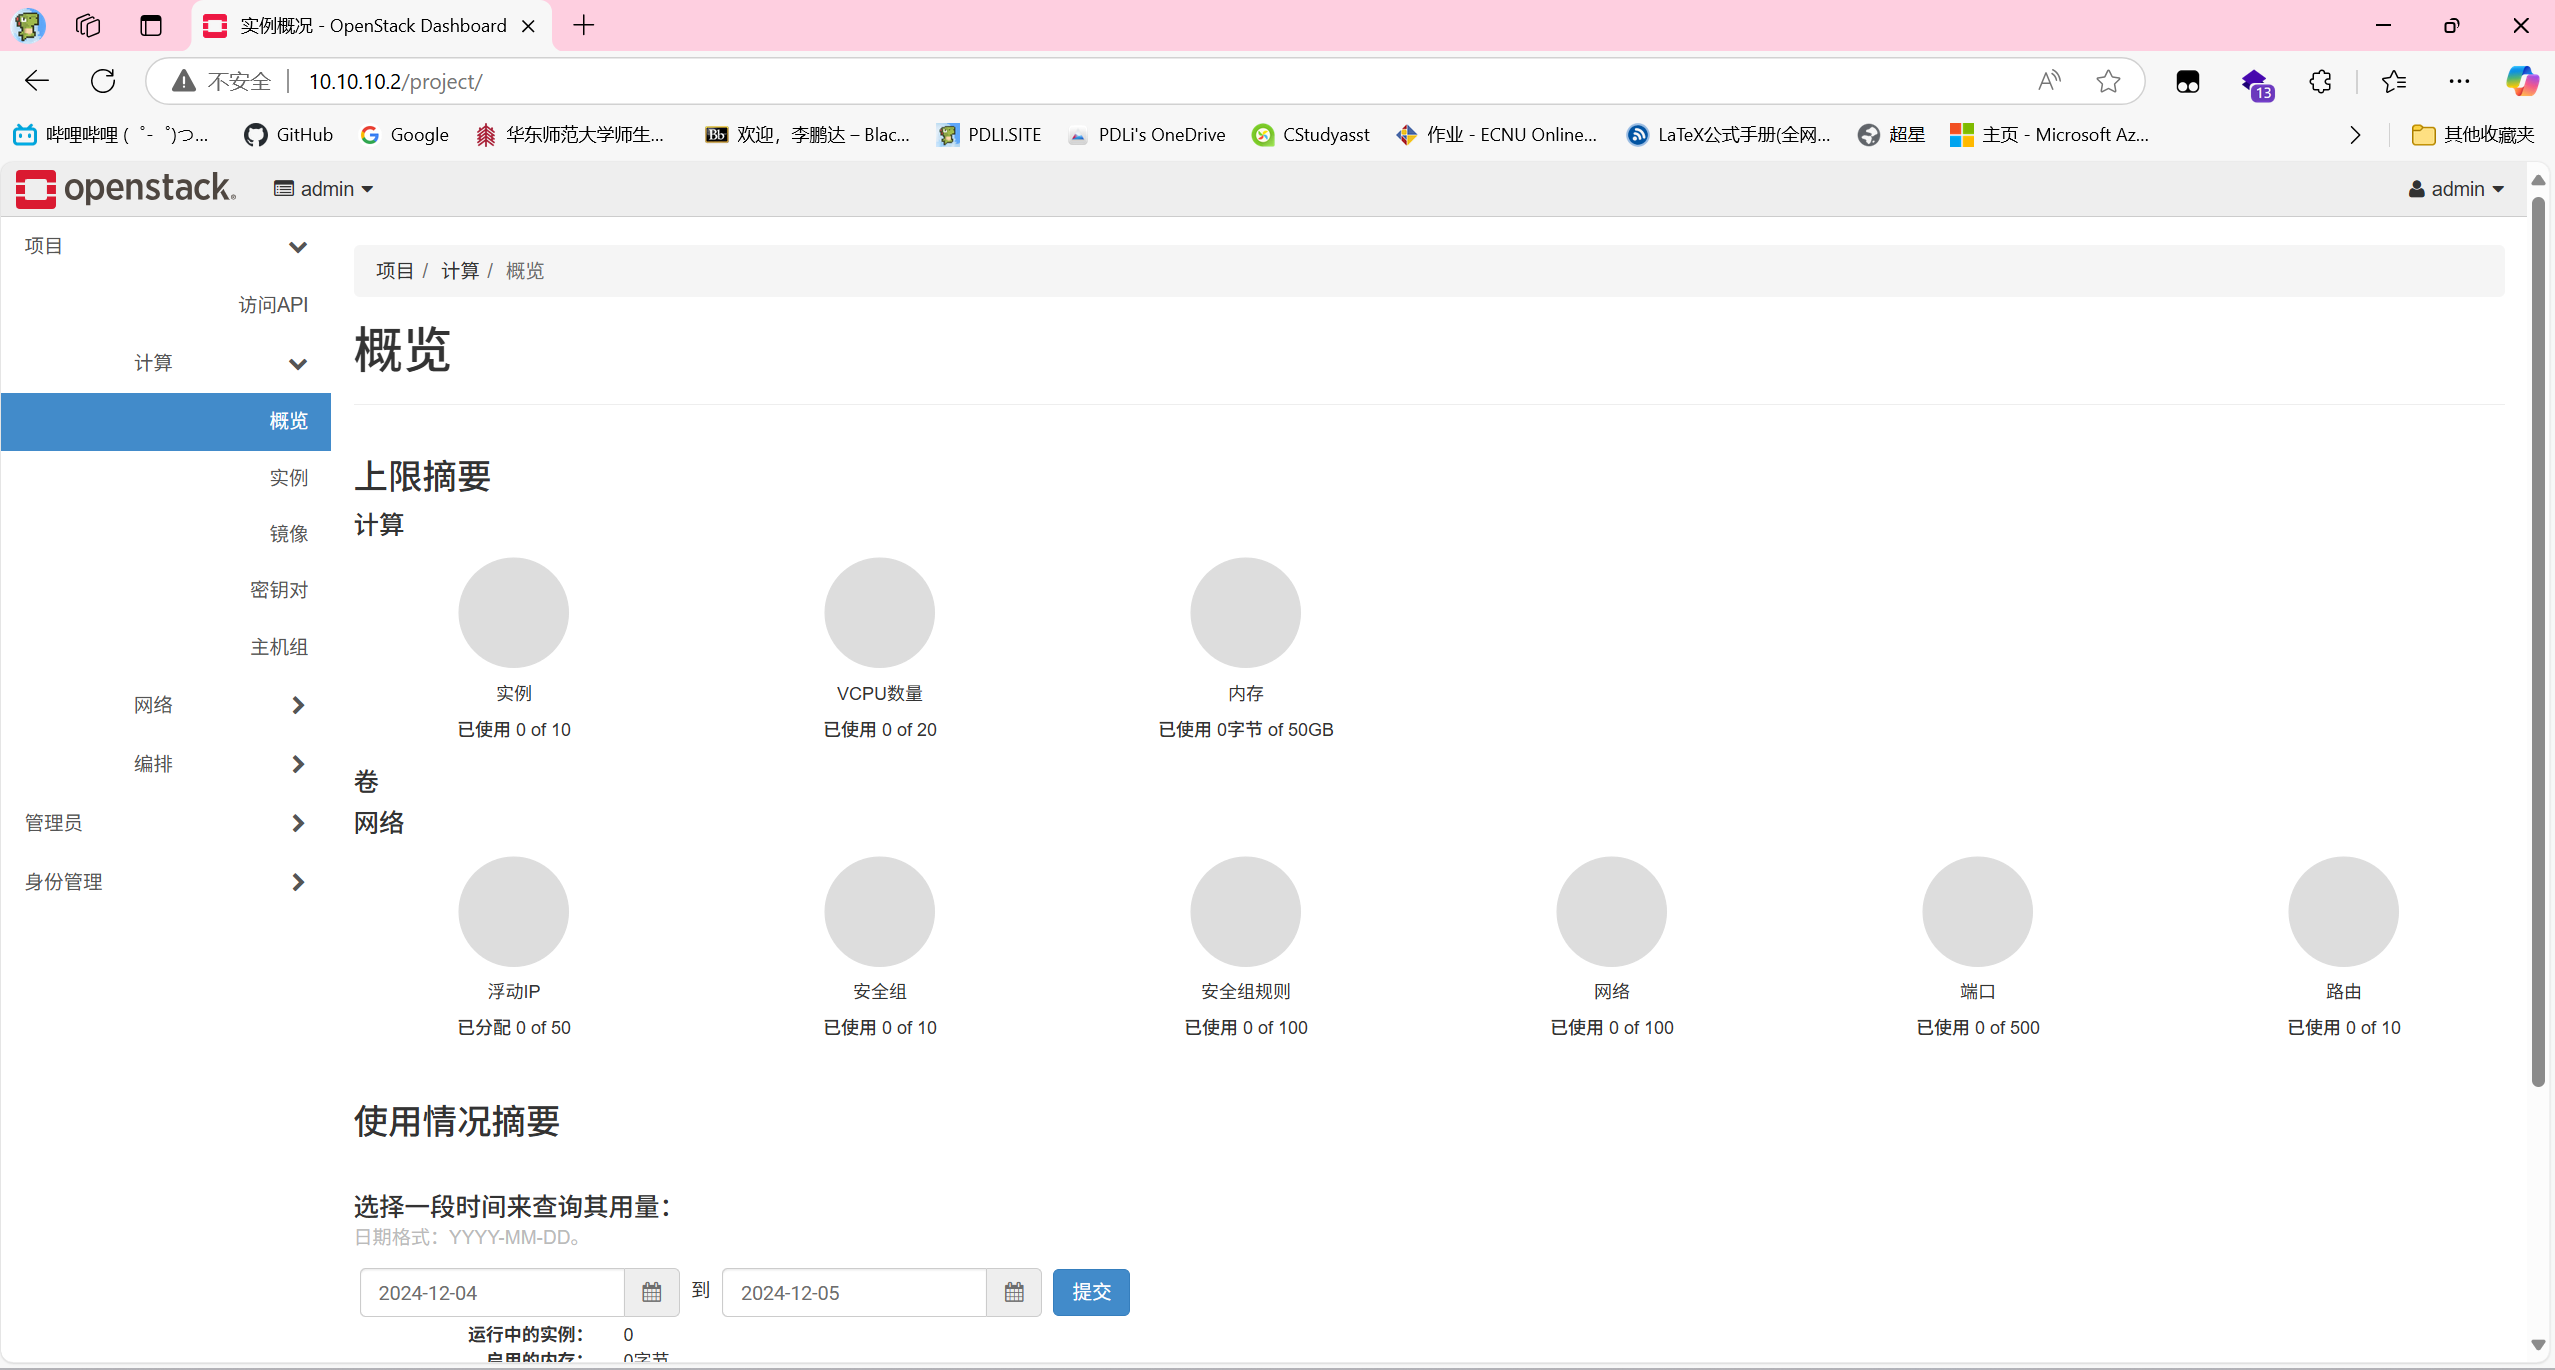
\includegraphics[width=0.85\textwidth]{img/7.9.png}
    \caption{OpenStack控制台}
\end{figure}

\subsection{创建的实例}

\begin{figure}[H]
    \centering
    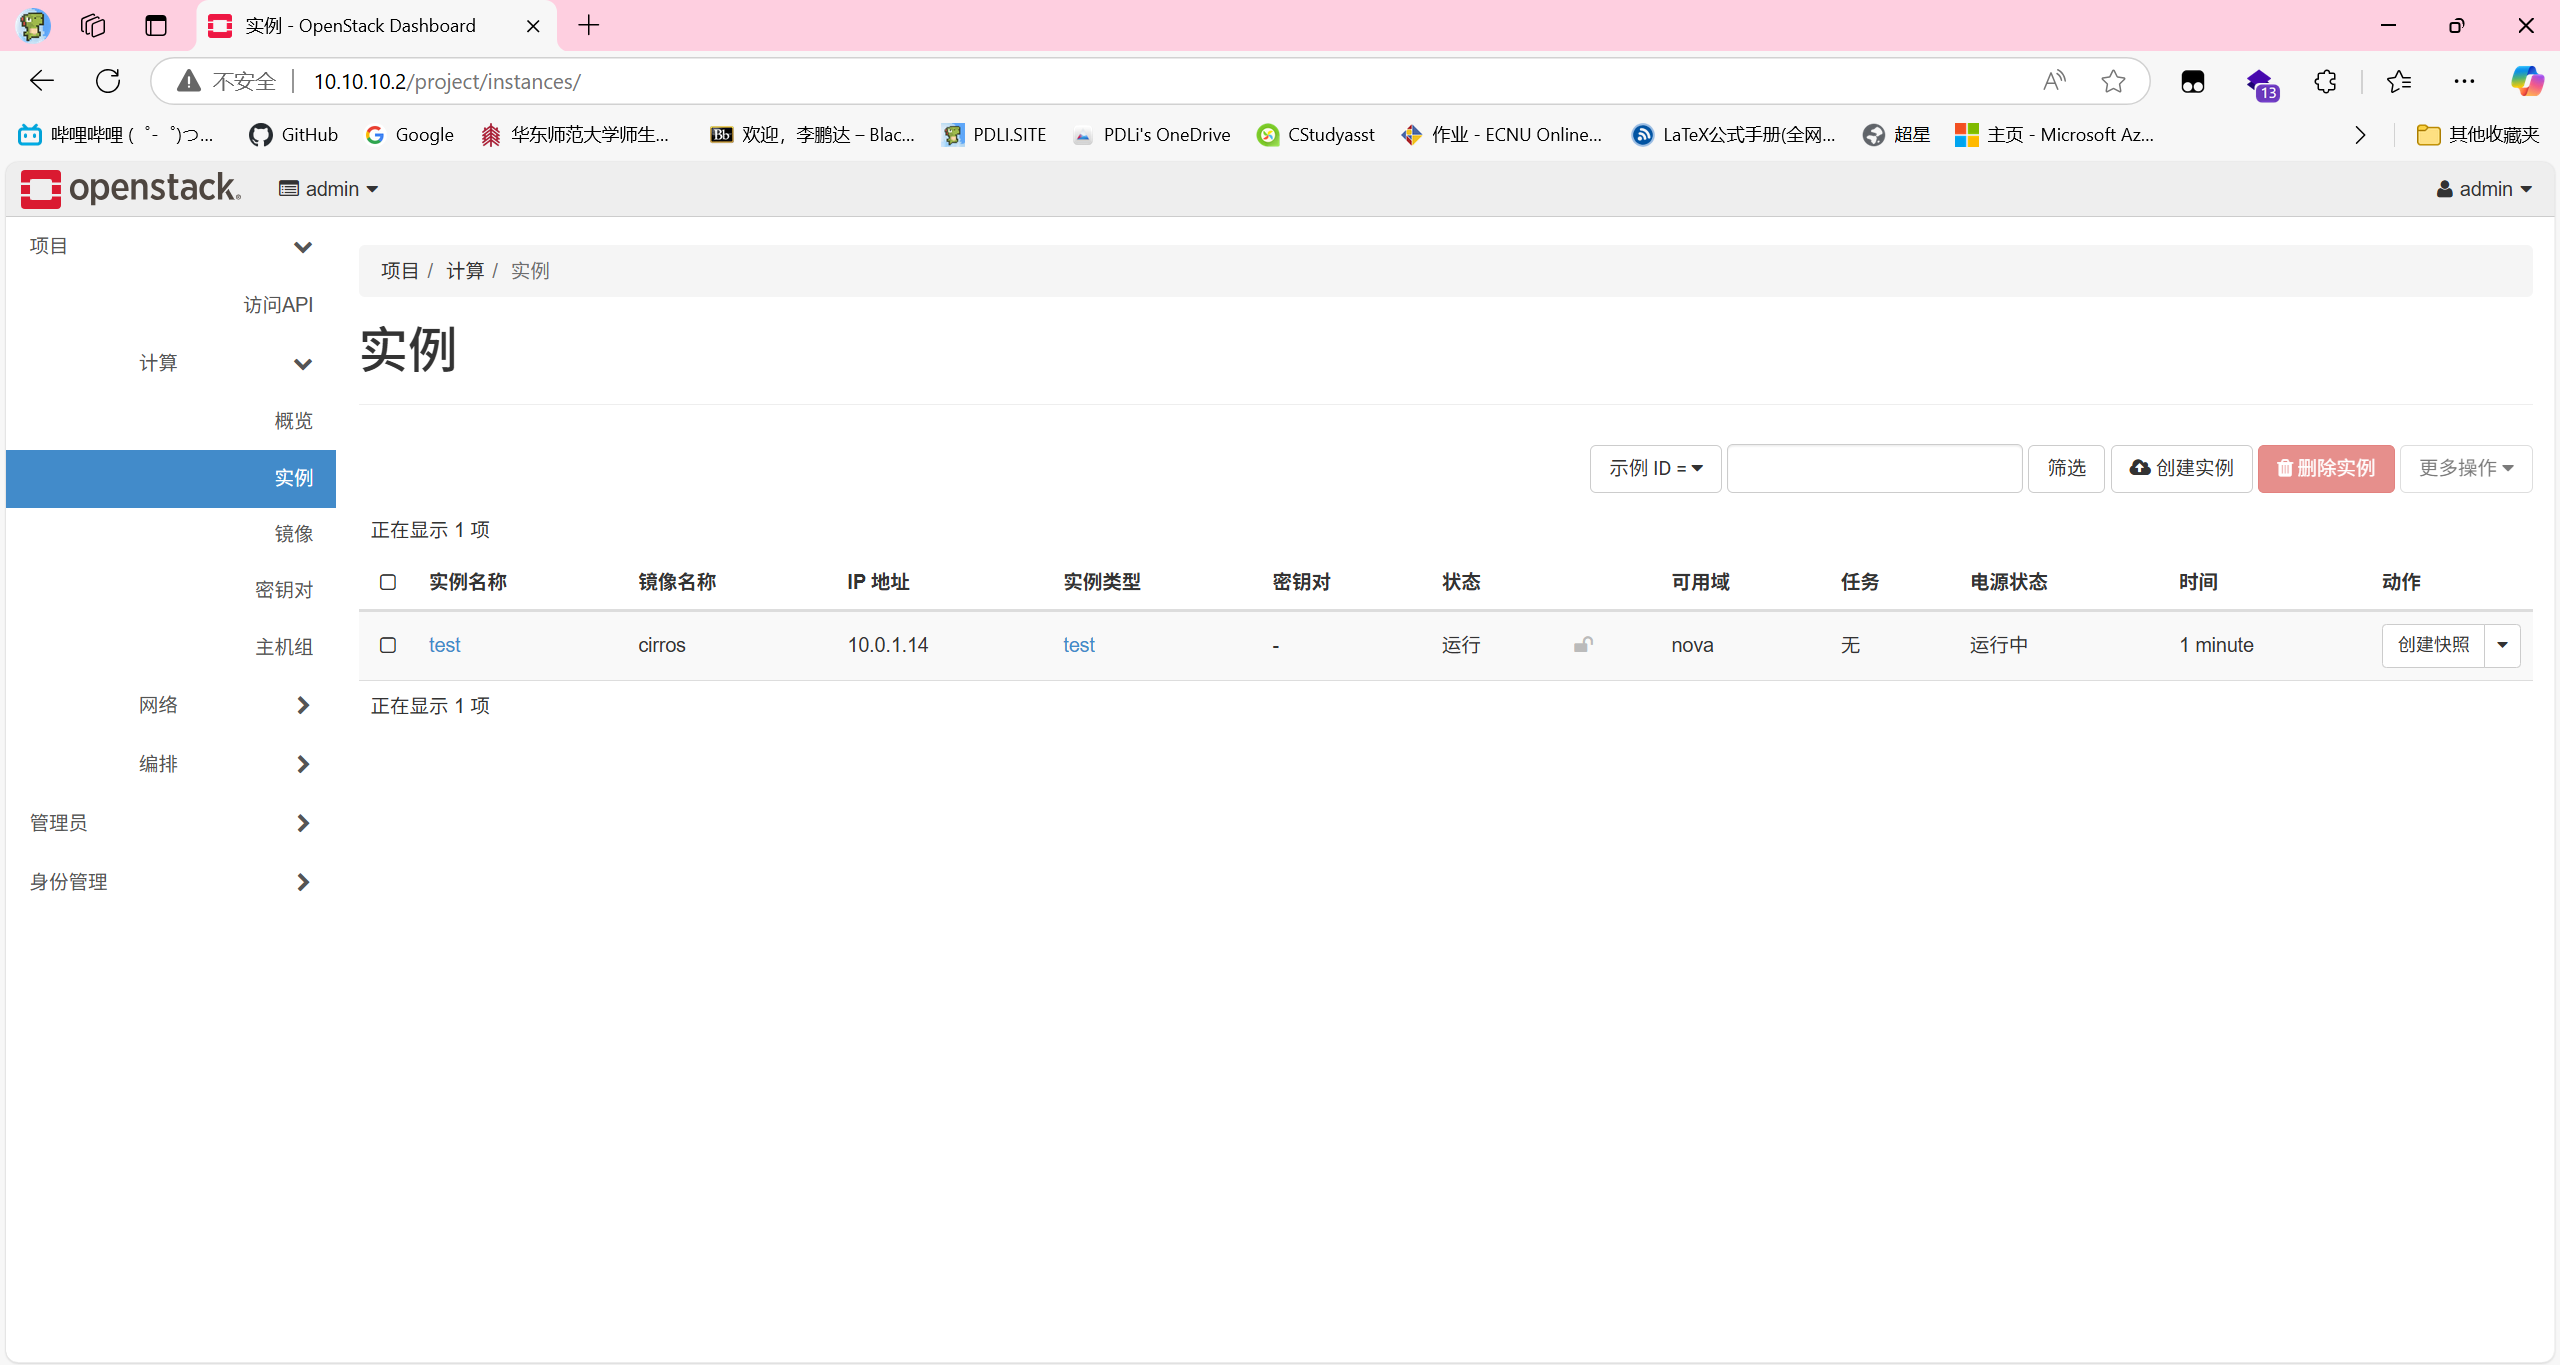
\includegraphics[width=0.85\textwidth]{img/11.4.png}
    \caption{创建的实例}
\end{figure}

\section{实验总结}

通过本次实验,我成功安装和配置了OpenStack云平台,并创建了一个实例。在实验过程中,我学会了如何在虚拟机中安装OpenStack,并通过OpenStack创建实例。实验过程比较顺利,没有遇到问题,但需要耐心等待安装过程。在实验中,我还学会了如何使用OpenStack的一些基本功能,如创建镜像、实例类型、网络等。总的来说,本次实验收获颇丰,对OpenStack有了更深入的了解。

\end{document}